\documentclass[a4paper,12pt, oneside]{book}

% \usepackage{fullpage}
\usepackage[italian]{babel}
\usepackage[utf8]{inputenc}
\usepackage{amssymb}
\usepackage{amsthm}
\usepackage{graphics}
\usepackage{amsfonts}
\usepackage{listings}
\usepackage{amsmath}
\usepackage{amstext}
\usepackage{engrec}
\usepackage{rotating}
\usepackage{verbatim}
\usepackage[safe,extra]{tipa}
% \usepackage{showkeys}
\usepackage{multirow}
\usepackage{hyperref}
\usepackage{microtype}
\usepackage{fontspec}
\usepackage{enumerate}
\usepackage{physics}
\usepackage{braket}
\usepackage{marginnote}
\usepackage{pgfplots}
\usepackage{cancel}
\usepackage{polynom}
\usepackage{booktabs}
\usepackage{enumitem}
\usepackage{framed}
\usepackage{pdfpages}
\usepackage{pgfplots}
\usepackage{algorithm}
% \usepackage{algpseudocode}
\usepackage[cache=false]{minted}
\usepackage{mathtools}
\usepackage[noend]{algpseudocode}
\newcommand*{\bfrac}[2]{\genfrac{}{}{0pt}{}{#1}{#2}}

\usepackage{tikz}\usetikzlibrary{er}\tikzset{multi  attribute /.style={attribute
    ,double  distance =1.5pt}}\tikzset{derived  attribute /.style={attribute
    ,dashed}}\tikzset{total /.style={double  distance =1.5pt}}\tikzset{every
  entity /.style={draw=orange , fill=orange!20}}\tikzset{every  attribute
  /.style={draw=MediumPurple1, fill=MediumPurple1!20}}\tikzset{every
  relationship /.style={draw=Chartreuse2,
    fill=Chartreuse2!20}}\newcommand{\key}[1]{\underline{#1}}
\usetikzlibrary{arrows.meta}
\usetikzlibrary{decorations.markings}
\usetikzlibrary{arrows,shapes,backgrounds,petri}
\tikzset{
  place/.style={
    circle,
    thick,
    draw=black,
    minimum size=6mm,
  },
  transition/.style={
    rectangle,
    thick,
    fill=black,
    minimum width=8mm,
    inner ysep=2pt
  },
  transitionv/.style={
    rectangle,
    thick,
    fill=black,
    minimum height=8mm,
    inner xsep=2pt
  }
} 
\usetikzlibrary{automata,positioning,chains,fit,shapes}
\usepackage{fancyhdr}
\pagestyle{fancy}
\fancyhead[LE,RO]{\slshape \rightmark}
\fancyhead[LO,RE]{\slshape \leftmark}
\fancyfoot[C]{\thepage}
\usepackage[usenames,dvipsnames]{pstricks}
\usepackage{epsfig}
\usepackage{pst-grad} % For gradients
\usepackage{pst-plot} % For axes
\usepackage[space]{grffile} % For spaces in paths
\usepackage{etoolbox} % For spaces in paths
\makeatletter % For spaces in paths
\patchcmd\Gread@eps{\@inputcheck#1 }{\@inputcheck"#1"\relax}{}{}
\makeatother
\usepackage{lipsum}
\DeclareSymbolFont{symbolsC}{U}{txsyc}{m}{n}
\DeclareMathSymbol{\strictif}{\mathrel}{symbolsC}{74}
\title{Fondamenti Logico Matematici dell'Informatica}
\author{UniShare\\\\Davide Cozzi\\\href{https://t.me/dlcgold}{@dlcgold}}
\date{}

\pgfplotsset{compat=1.13}
\begin{document}
\maketitle

\definecolor{shadecolor}{gray}{0.80}
\setlist{leftmargin = 2cm}
\newtheorem{teorema}{Teorema}
\newtheorem{definizione}{Definizione}
\newtheorem{esempio}{Esempio}
\newtheorem{corollario}{Corollario}
\newtheorem{lemma}{Lemma}
\newtheorem{osservazione}{Osservazione}
\newtheorem{nota}{Nota}
\newtheorem{esercizio}{Esercizio}
\algdef{SE}[DOWHILE]{Do}{doWhile}{\algorithmicdo}[1]{\algorithmicwhile\ #1}
\tableofcontents
\renewcommand{\chaptermark}[1]{%
  \markboth{\chaptername
    \ \thechapter.\ #1}{}}
\renewcommand{\sectionmark}[1]{\markright{\thesection.\ #1}}
\newcommand{\floor}[1]{\lfloor #1 \rfloor}
\newcommand{\MYhref}[3][blue]{\href{#2}{\color{#1}{#3}}}%
\chapter{Introduzione}
\textbf{Questi appunti sono presi a lezione. Per quanto sia stata fatta
  una revisione è altamente probabile (praticamente certo) che possano
  contenere errori, sia di stampa che di vero e proprio contenuto. Per
  eventuali proposte di correzione effettuare una pull request. Link: }
\url{https://github.com/dlcgold/Appunti}.\\
\chapter{Dimostrazioni come Algoritmi}
Parliamo in primis del \textbf{paradigma dimostrazioni = algoritmi}.\\
Prendiamo come \textit{linguaggio di specifica} un \textbf{linguaggio
  del prim'ordine con identità}.
\begin{shaded}
  Si riportano alcune definizioni utili in \textit{logica matematica} tratte da
  Wikipedia: 
  \begin{definizione}
    Definiamo \textbf{linguaggio del primo ordine} come un linguaggio formale
    che serve per gestire meccanicamente enunciati e ragionamenti che
    coinvolgono i connettivi logici, le relazioni e i quantificatori $\forall$ e
    $\exists$.\\
    Si ha che ``del primo ordine'' indica che c'è un insieme di riferimento e i
    quantificatori possano riguardare solo gli elementi di tale insieme e non i
    sottoinsiemi (posso dire ``per tutti gli elementi'' ma non ``per tutti i
    sottoinsiemi''). Tale linguaggio è caratterizzato da:
    \begin{itemize}
      \item un \textbf{alfabeto di simboli} per variabili, costanti, predicati,
      funzioni, connettivi, quantificatori o punteggiatura 
      \item un \textbf{insieme di termini} per denotare gli elementi
      dell'insieme in analisi
      \item un \textbf{insieme di formule ben formate (\textit{FBF})} ovvero un
      insieme di stringhe composte di simboli dell'alfabeto che vengono
      considerate sintatticamente corrette 
    \end{itemize}
  \end{definizione}
  \begin{definizione}
    Definiamo \textbf{sistema assiomatico} come un insieme di assiomi che
    possono essere usati per dimostrare teoremi. Una teoria matematica consiste
    quindi in una assiomatica e tutti i teoremi che ne derivano.  
  \end{definizione}
  \begin{definizione}
    Definiamo un sistema formale come una formalizzazione rigorosa e completa
    della nozione di sistema assiomatico costituito da:
    \begin{itemize}
      \item un alfabeto
      \item una grammatica che specifica quali sequenze finite dei simboli
      dell'alfabeto corrispondono ad una FBF. La grammatica deve essere
      ricorsiva, nel senso che deve esistere un algoritmo per decidere se una
      sequenza di simboli è o meno una formula ben formata 
      \item un sottoinsieme delle FBF che sono gli assiomi. L'insieme degli
      assiomi è ricorsivo
      \item le regole di inferenze che associano formule ben formate ad n-uple
      di formule ben formate
    \end{itemize}
  \end{definizione}
  \begin{definizione}
    Definiamo gli \textbf{assiomi di Peano} come un gruppo di assiomi ideati al
    fine di definire assiomaticamente l'insieme dei numeri naturali:
    \begin{itemize}
      \item esiste un numero naturale: 0 (alternativamente 1 se si vuole escludere
      0):
      \[0/1\in \mathbb{N}\]
      \item ogni naturale ha un naturale come successore. Ho quindi una funzione
      ``successore'' tale che:
      \[S:\mathbb{N}\to\mathbb{N}\]
      \item numeri diversi hanno successori diversi, ovvero:
      \[x\neq y\to S(x)\neq S(y)\]
      \item 0 (o alternativamente 1) non è il successore di alcun naturale,
      ovvero:
      \[S(x)\neq 0, \forall x\in \mathbb{N}\]
      \item ogni sottoinsieme di numeri naturali che contenga lo zero e il
      successore di ogni proprio elemento coincide con l'intero insieme dei
      numeri 
      naturali. Ovvero dato $U\subseteq \mathbb{N}$ tale che:
      \begin{itemize}
        \item $0\in U$
        \item $x\in U\to S(x)\in U$
      \end{itemize}
      allora:
      \[U=\mathbb{N}\]
      Tale assioma è detto \textbf{assioma dell'induzione} o \textbf{principio di
        induzione} 
    \end{itemize}
  \end{definizione}
  \begin{definizione}
    In una teoria del primo ordine si chiama \textbf{chiusura universale} di una
    formula ben formata $A(x_1,\ldots,x_n)$, con $x_1,\ldots,x_n$ variabili
    libere, la formula:
    \[\forall x_1\forall x_2\forall x_n\,\,A(x_1,\ldots,x_n)\]
    ottenuta premettendo un quantificatore universale su ogni variabile libera. 
  \end{definizione}
  \begin{definizione}
    Definiamo, in logica matematica, \textbf{aritmetica di Peano (\textit{PA})}
    come una teoria del primo 
    ordine che ha come assiomi propri una versione degli \textbf{assiomi di
      Peano} 
    espressi nel linguaggio del primo ordine. Si ha quindi che il linguaggio di
    PA 
    è il linguaggio dell'aritmetica del primo ordine con i seguenti simboli:
    \begin{itemize}
      \item vari simboli per le variabili: $x$, $y$, $z$, $x_1$ etc$\ldots$
      \item costanti individuali: $0$ etc$\ldots$
      \item simboli per funzioni unarie: $S$
      \item simboli per funzioni binarie $+$, $\times$ ($+(x,y)$ si indica anche
      con $x+y$ e analogamente si fa per $\times$)
      \item simboli per relazioni unarie: $=$
      \item simboli per connettivi logici, quantificatori e parentesi
    \end{itemize}
    Gli assiomi di PA sono costituiti da:
    \begin{itemize}
      \item gli assiomi logici
      \item gli assiomi per l'uguaglianza
      \item i seguenti assiomi propri (che ``traducono'' nella logica di Peano
      gli assiomi di Peano):
      \begin{itemize}
        \item $\forall x\neg(S(x)=0)$
        \item $\forall x\forall y(S(x)=S(y)\to x=y)$
        \item $\forall x(x+0=x)$
        \item $\forall x\forall y(x+S(y)=S(x+y))$
        \item $\forall x(x\times 0 =0)$
        \item $\forall x\forall y(x\times S(y)=(x\times y)+x)$
      \end{itemize}
    \end{itemize}
    Agli assiomi propri si aggiunge anche il seguente assioma proprio:
    {\footnotesize{\[(\phi(0,x_1,\ldots,x_n)\land(\forall
      x(\phi(x,x_1,\ldots,x_n)\to\phi(S(x),x_1,\ldots,x_n))\to\forall 
      x\phi(x,x_1,\ldots,x_n)\]}}
    per ogni FBF $\phi(x,x_1,\ldots,x_n)$ di cui
    $x,x_1,\ldots,x_n$ sono variabili libere. Questo è uno schema di assiomi
    detto \textbf{schema di induzione} e si ha un assioma per ogni FBF
    $\phi$ 
  \end{definizione}
  \begin{definizione}
    Definiamo, in logica classica, il \textbf{principio del terzo escluso} che
    stabilisce che una proposizione e la sua negazione hanno valore opposto, non
    avendo una ``terza opzione''. In logica classica è una \textbf{tautologia}.
  \end{definizione}
  \begin{definizione}
    Un termine è un \textbf{termine chiuso} sse non contiene delle variabili
    individuali.  
  \end{definizione}
  \begin{definizione}
    Una \textbf{formula chiusa} è una formula costruita nel linguaggio dei
    predicati in cui o non compaiono variabili o tutte le variabili presenti
    sono vincolate a un quantificatore e sono dunque variabili legate. 
  \end{definizione}
\end{shaded}
\begin{esempio}
  Vediamo qualche esempio:
  \[\forall x,y\in\mathbb{N},\,\,\exists z\in\mathbb{N}\mbox{ t.c. }
    mcd(x,y,z)\]
  ovvero $z$ è l'\textit{mcd} di $x$ e $y$.\\
  Un altro esempio:
  \[\forall x\in \mathbb{N},\,\,\exists y\in \mathbb{N}\mbox{ t.c. }
    fatt(x,y)\]
  ovvero $y$ è il fattoriale di $z$.
\end{esempio}
Formule come quelle dell'esempio possono essere lette come \textbf{specifiche
  del problema di trovare un algoritmo totalmente corretto} che calcoli il
risultato di tale problema per ogni input valido. Questa lettura non è implicita
nella logica classica, dove non è richiesto di stabilire come viene prodotto il
risultato. Si ha quindi a che fare con una lettura di un problema algoritmico di
interesse per un informatico.\\
Le \textbf{dimostrazioni} di questa tipologia di formule, nell'ambito
dell'\textbf{aritmetica di Peano (\textit{PA})}, sono quindi interpretabili come
gli algoritmi che calcolano le funzioni specificate. \\
Come \textit{vantaggi} di questa ``atteggiamento'' si ha che:
\begin{itemize}
  \item l'attenzione si concentra su costruire la dimostrazione, sui passi
  dimostrativi, e non sulla stesura del codice
  \item i passi elementari della dimostrazione sono automatici
  \item la correttezza della dimostrazione è verificabile in modo automatico
  \item l'estrazione/sintesi dell'algoritmo dalla dimostrazione è diretta. Una
  volta che si ha la dimostrazione corretta si può estrarre direttamente
  l'algoritmo. Tale algoritmo è totalmente corretto rispetto alla specifica
\end{itemize}
La difficoltà si trasferisce dall'ambito convenzionale della programmazione e
codifica dell'algoritmo in se alla costruzione dimostrazione e dei passi
dimostrativi.\\
Si hanno quindi anche degli \textit{svantaggi}, abbastanza problematici:
\begin{itemize}
  \item l'algoritmo ottenuto non è ottimale rispetto al problema. Rispetto a
  questo bisognerebbe capire come incorporare ``più semantica'' del problema da
  risolvere nella dimostrazione stessa
  \item il formalismo e il linguaggio delle dimostrazioni sono ``lontani'' da
  quelli usati usualmente nella pratica informatica
\end{itemize}
\textbf{Non tutte le dimostrazioni sono direttamente interpretabili come
  algoritmi}. Per vedere questa cosa prendiamo un esempio famoso di formula da
dimostrare in analisi.
\begin{esempio}[esempio di Troelstra]
  Esistono due numeri irrazionali $n$ e $m$ tali che $n^m$ è razionale. In
  termini di formula del primo ordine si ha quindi:
  \[\exists n,m\in\{\mathbb{R}/\mathbb{Q}\}\mbox{ t.c. }n^m\in\mathbb{Q}\]
  Cerchiamo di capire se:
  \[\sqrt{2}^{\sqrt{2}}\in \mathbb{Q}\mbox{ o }\sqrt{2}^{\sqrt{2}}\not\in
    \mathbb{Q}\]
  Vediamo quindi i due casi (sono solo due per il principio del terzo escluso):
  \begin{enumerate}
    \item assumo $\sqrt{2}^{\sqrt{2}}\in \mathbb{Q}$ e pongo $n=m=\sqrt{2}$
    avendo trovato due numeri irrazionali $n$ e $m$ tali per cui
    $n^m\in\mathbb{Q}$ 
    \item assumo $\sqrt{2}^{\sqrt{2}}\not\in \mathbb{Q}$ e pongo
    $n=\sqrt{2}^{\sqrt{2}}$ e $m=\sqrt{2}$. Ne segue che:
    \[n^m=\left(\sqrt{2}^{\sqrt{2}}\right)^{\sqrt{2}}=(\sqrt{2})^2=2\in\mathbb{Q}\] 
    e quindi ho due numeri irrazionali $n$ e $m$ tali per cui $n^m\in\mathbb{Q}$
  \end{enumerate}
  Non possiamo essere soddisfatti di questa dimostrazione. Non veniamo a
  conoscenza, tramite la dimostrazione, che $\sqrt{2}^{\sqrt{2}}$ sia o meno
  razionale. Non possiamo capirlo in quanto assumo il terzo escluso e quindi non
  so quale dei due casi sia valido, non abbiamo un ``esiste'' costruttivo
  ($\exists n,m\in \{\mathbb{R}/\mathbb{Q}\}$) in quanto non sappiamo se
  $\sqrt{2}^{\sqrt{2}}$ è razionale o meno. Nonostante ciò al dimostrazione sta
  perfettamente ``in piedi'' ma non esibisce $n$ e $m$ in quanto non determina
  se $\sqrt{2}^{\sqrt{2}}\in\mathbb{Q}$.
\end{esempio}
Quanto successo nell'esempio di Troelstra non può succedere in un
\textbf{sistema costruttivo}.
\begin{definizione}
  Definiamo \textbf{sistema costruttivo} un sistema dove si hanno come
  \textit{requisiti minimali}: 
\begin{itemize}
  \item $S\vdash A\lor B\to S\vdash A\mbox{ oppure } S\vdash B$ quindi se
  nel sistema dimostro $A\lor B$ allora nel sistema dimostro $A$ o dimostro $B$,
  con $A$ e $B$ formule chiuse. Questa è la \textbf{disjunction property
    (\textit{DP})}  
  \item $S\vdash\exists xA(x)\to S\vdash A(t)$ quindi se ho dimostrato un
  esistenziale allora deve esistere un termine chiuso $t$ per cui dimostro
  $A(t)$ nel sistema. Questa è la \textbf{explicitly definibility property
    (\textit{EDP})}, detta anche \textbf{existence/witness property}
\end{itemize}
\end{definizione}
La logica classica quindi \textbf{non è un sistema costruttivo} perché in logica
classica riesco sempre a dimostrare $A\lor\neg A$ mentre nell'esempio di
Troelstra si nota come non si possa dimostrare né $A$ né $\neg A$. Quindi da una
dimostrazione classica di $A\lor\neg A$ io non tiro fuori una dimostrazione
classica di $A$ oppure una dimostrazione classica di $\neg A$ quindi non vale la
DP. Inoltre non vale nemmeno la EDP, ho dimostrato l'esistenza di $n$ e $m$ (che
sono termini chiusi) ma non ho trovato se vale la proprietà che siano
irrazionali. La logica classica quindi non è una logica costruttiva.
\section{Interpretazione BHK}
Passiamo quindi ad una semantica informale che per ogni costante logica associa
una condizione per la sua \textit{costruibilità}. Questa è
\textbf{l'interpretazione Brouwer-Heyting-Kreisel (\textit{BHK})}.
\begin{definizione}
  Presa una costruzione $\pi$ per questa semantica proposizionale si ha che:
  \begin{itemize}
    \item $\pi(A\land B)=\pi'(A)\mbox{ e } \pi''(B)$ ovvero una costruzione di
    $A\land B$ è uguale ad un'altra costruzione di $A$ \textbf{e} un'altra
    ancora di $B$ 
    \item $\pi(A\lor B)=\pi'(A)\mbox{ o } \pi''(B)$ ovvero una costruzione di
    $A\lor B$ è uguale ad un'altra costruzione di $A$ \textbf{o} un'altra ancora
    di $B$
    \item $\pi(A\to B)$ è una funzione  (o un funzionale, ovvero un
    insieme di funzioni) $f$ che associa ad ogni
    costruzione $\pi'(A)$ una costruzione $\pi''(B)$ tale che
    $\pi''=f(\pi')$. Quindi $f$ associa costruzioni di $A$ a costruzioni di $B$
    \item $\pi(\neg A)$ è una costruzione $\pi'$ di $A\to\bot$
  \end{itemize}
  Lato semantica predicativa si ha che, dato un dominio $D$ per la variabile
  $x$: 
  \begin{itemize}
    \item $\pi(\exists xA(x))=\langle c,\pi'\rangle|\,c\in D\mbox{ e
    }\pi'(A(c))$ quindi è uguale ad una coppia $\langle c,\pi'\rangle$ tale che
    $c$ appartiene al dominio e $\pi'$ è una costruzione effettiva di $A(c)$
    \item $\pi(\forall xA(x))=$ è una funzione $f$ che associa ad ogni elemento
    $c\in D$ una costruzione $\pi'(A(c))$ tale che $\pi'=f(c)$
  \end{itemize}
\end{definizione}
Questa semantica ``naive'' ha alcune problematiche/aporie:
\begin{itemize}
  \item la BHK non specifica la costruzione di una formula atomica
  \item la BHK non dimostra il falso infatti nella costruzione di $\neg$
  associamo la costruzione del $\neg A$ a quella dell'implicazione, che è una
  costruzione che associa costruzioni di $A$ e costruzioni di $B$ e quindi
  nessuna costruzione potrebbe avere il falso
\end{itemize}
Bisognerà quindi chiarire alcune restrizioni dell'interpretazione BHK.\\
Si hanno varie semantiche per il costruttivismo che hanno ``precisato'' la BHK:
\begin{itemize}
  \item la semantica della \textbf{realizzabilità ricorsiva} di Kleene
  \item la semantica dell'\textbf{interpretazione dialettica} di G\"{o}del
  \item la semantica delle \textbf{prove possibili} di Prawitz
  \item la semantica dei \textbf{problemi finiti} di Medvedev
\end{itemize}
Queste 4 semantiche sono coerenti con la BHK e quindi sono \textbf{semantiche
  del costruttivismo}.\\
Passiamo ora ad una definizione formale.
\begin{definizione}
  Definiamo come \textbf{sistema costruttivo} un sistema $S$:
  \[S=T+L\]
  dove:
  \begin{itemize}
    \item $T$ è una teoria con assiomi di forma particolare
    \item $L$ è una logica intuizionistica, che prendiamo come punto di partenza
    per il costruttivismo, con le sue estensioni
  \end{itemize}
  Non sempre comunque date $T$ e $L$ si ha che $S$ è un sistema costruttivo.
\end{definizione}
Un esempio di sistema costruttivo è dato dall'\textbf{aritmetica
  intuizionistica}, ovvero la PA interpretata all'interno della logica
intuizionistica. Altri esempi sono le \textbf{teorie con assiomi di Harrop},
teorie con assiomi $\forall\exists$ con matrice positiva priva di quantificatori
e con minimo modello di Herbrandt etc$\ldots$\\ 
Le clausole di Horn usate i Prolog hanno un
modello minimo di Herbrandt e hanno  assiomi $\forall\exists$ con matrice
positiva priva di quantificatori dove $\exists$ viene eliminato attraverso
skolemizzazione e il $\forall$ è implicito nelle regole del programma in quanto
tutte le $X$, $Y$ etc$\ldots$ si intendono quantificati universalmente.\\
Quindi la parte assiomatica di una teoria non basta a rendere costruttivo il
sistema anche se la logica è costruttiva. Tuttavia se si restringono le
assiomatizzazioni con formule del primo ordine di tipo particolare si possono
ottenere sistemi costruttivi in cui vale come minimo la \textit{DP} e la
\textit{EDP}.
\section{Deduzione naturale}
Vediamo un accenno della \textbf{deduzione naturale} ovvero di un
\textbf{calcolo diretto} (quindi differente dal calcolo indiretto dei
tableaux). Nella deduzione naturale si ha, per ogni connettivo, una
\textbf{regola di introduzione} $i$ e una \textbf{regola di eliminazione}
$e$. Ad esempio se ho $A$ e $B$ come premesse posso introdurre l'and con la
regola di introduzione dell'and: 
\[\frac{A\,\,\,\,B}{A\land B}i\land\]
Se invece ho $A\land B$ come premessa posso usare la regola di eliminazione
dell'and, producendo:
\[\frac{A\land B}{A}e\land\mbox{ oppure }\frac{A\land B}{B}e\land\]
Avendo quindi due regole di eliminazione per l'and.\\
Passiamo all'or. Ho due regole di introduzione:
\[\frac{A}{A\lor B}i\lor\mbox{ oppure }\frac{B}{A\lor B}i\lor\]
L'eliminazione della or è complessa e verrà trattata più avanti ma è della
forma:
\[\frac{A\lor B\,\,\,\,C\,\,\,\,C}{C}e\lor\]
Dove si ha che se se ho $A\lor B$ come premessa e assumendo $A$ ho $C$ ma anche
assumendo $B$ ho $C$ posso eliminare l'or e ottenere $C$.\\
Passiamo all'implicazione. Se ho come assunzione $A$ e da $B$ riesco a
dimostrare $B$ allora posso introdurre l'implicazione:
\[\frac{\stackrel{\stackrel{[A]}{\cdots}}{B}}{A\to B}i\to\]
Per l'eliminazione ho che, tramite \textbf{modus ponens}:
\[\frac{A\to B\,\,\,\,A}{B}e\to\]
Abbiamo poi la \textbf{regola del falso} che dice che dal falso segue qualsiasi
cosa: 
\[\frac{\bot}{B}\bot\]
e la regola dell'eliminazione della negazione che dice che se assumo $\neg A$ e
ottengo il falso significa che si è ottenuta una contraddizione e quindi elimino
il $\neg$:
\[\frac{\stackrel{[\neg A]}{\bot}}{A}e\neg\]
Passiamo al $\forall$. Se ho dedotto $A(p)$ per $p$ generico posso introdurre il
$\forall$:
\[\frac{A(p)}{\forall xA(x)}i\forall\]
Se ho come assunzione $\forall xA(x)$ posso dedurre un qualsiasi $A(t)$:
\[\frac{\forall xA(x)}{A(t)}e\forall\]
Possiamo fare l'equivalente per l'$\exists$, dove se esiste $A(t)$ posso dedurre
l'esistenza di un certo $x$ per cui vale $A(x)$:
\[\frac{A(t)}{\exists xA(x)}i\exists\]
L'eliminazione dell'esiste è complessa e verrà trattata più avanti ma è della
forma:
\[\frac{\exists xA(x)\,\,\,\,\stackrel{[A(p)]}{C}}{C}e\exists\]
Dove assumendo $\exists xA(x)$, assumendo $A(p)$ con $p$ generico e riuscendo ad
ottenere $C$ da quest'ultima assunzione con una serie di restrizioni posso
ottenere $C$ eliminando $\exists$.\\
Una dimostrazione in deduzione naturale è modulare alle logiche che si vogliono
usare:
\begin{itemize}
  \item nelle dimostrazioni in logica classica utilizzo tutte le regole della
  deduzione naturale appena introdotte
  \item nelle dimostrazioni in logica intuizionistica non devo usare la regola
  di eliminazione della negazione
  \item  nelle dimostrazioni in logica minimale non devo usare la regola
  di eliminazione della negazione e nemmeno la regola che dal falso segue
  qualsiasi cosa
\end{itemize}
Possiamo quindi caratterizzare queste tre logiche e nelle ultime due, quella
intuizionistica e quella minimale, si può dimostrare che valgono DP e EDP mentre
non posso dire lo 
stesso per la logica classica. Si ha inoltre che:
\[\mbox{logica minimale}\subseteq\mbox{logica
    intuizionistica}\subseteq\mbox{logica classica}\]
Discorso diverso vale per le teorie, ovvero per i sistemi, dove
l'assiomatizzazione può fare la differenza portando anche fuori dalla
costruttività (se ad esempio assumo come assioma che $\forall xA(x)\lor\neg
A(x)$ e gli aggiungo la logica intuizionistica ottengo la logica classica che
non è costruttiva).\\
Una teoria specifica è l'aritmetica di Peano dove si hanno i seguenti assiomi:
\begin{itemize}
  \item $\forall x\neg(S(x)=0)$
  \item $\forall x\forall y(S(x)=S(y)\to x=y)$
  \item $\forall x(x+0=x)$
  \item $\forall x\forall y(x+S(y)=S(x+y))$
  \item $\forall x(x\times 0 =0)$
  \item $\forall x\forall y(x\times S(y)=(x\times y)+x)$
\end{itemize}
Dove si ha la regola d'identità che in realtà sono due, ovvero $id1$ e $id2$:
\[\frac{}{x=x}id1\mbox{ e } \frac{x=y\,\,\,\,A(x)}{A(y)}id2\]
Dove si ha anche il principio/regola d'induzione:
\[\frac{A(0)\,\,\,\,\stackrel{\stackrel{[A(j)]}{\cdots}}{A(S(j))}}{A(t)}ind\]
Dove se dimostro $A(0)$ e assunto $A(j)$ dimostro il successore di $A(j)$ allora
posso dedurre $A(t),\forall t$.
\begin{esempio}
  Vediamo ora un esempio con degli assiomi specifici, costruttivi:
  \begin{itemize}
    \item $pari(0)$
    \item $\forall x(pari(x)\to \neg pari(S(x)))$
    \item $\forall x(\neg pari(x)\to pari(S(x)))$
  \end{itemize}
  Quindi si ha che se $x$ è apri non lo è il successore e se $x$ non è pari lo è
  il successore. Assumiamo inoltre che 0 sia pari.\\
  \textup{Scritta così potrebbe essere riscritta ``1:1'' in Prolog.}\\
  Cerchiamo quindi di dimostrare che che:
  \[\forall x(pari(x)\lor \neg pari(x))\]
  che si può pensare si un terzo escluso e quindi valga sempre. Questa formula,
  a 
  livello di specifica, va letta come una funzione ``per ogni numero naturale
  costruisce $pari(x)$ o $\neg pari(x)$'' quindi costruisce o la parte sinistra
  o 
  la parte destra. Quindi la formula si può leggere come la specifica di
  algoritmo 
  che per ogni naturale mi dice se vale la parte sinistra o la parte destra
  dell'or e quindi è un algoritmo di decisione effettivo che per ogni naturale
  ti 
  dice se è pari o non è pari. Questa è un'interpretazione diversa da quella
  classica. \\
  Posso quindi fare una dimostrazione per induzione.\\
  Il \textbf{caso base} è, chiamando $pari$ $p$, assunto per assioma $p(0)$ e
  usando l'introduzione dell'or:
  \[\frac{p(0)}{p(0)\lor \neg p(0)}i\lor\]
  Passo al \textbf{caso passo}.\\
  Assumo per ipotesi induttiva $p(j)\lor \neg p(j)$ e assumiamo $\forall
  x(p(x)\lor \neg p(S(x)))$ che è un altro degli assiomi. Procedo eliminando il
  $\forall$:
  \[\frac{\forall x(p(x)\lor \neg p(S(x)))}{p(j),p(j)\to\neg
      p(S(j))}e\forall\]
  procedo quindi eliminando l'implicazione:
  \[\frac{p(j),p(j)\to\neg
      p(S(j))}{\neg p(S(j))}e\to\]
  e continuo inserendo l'or:
  \[\frac{\neg p(S(j))}{p(S(j))\lor\neg p(S(j))}i\lor\]
  Analogamente faccio per l'altro assioma $\forall x(\neg p(x)\lor p(S(x)))$:
  \[\frac{\forall x(\neg p(S(x) )\lor  p(S(x)))}{\neg p(j),\neg p(j)\to
      p(S(j))}e\forall\]
  \[\frac{\neg p(j),\neg p(j)\to
      p(S(j))}{p(S(j))}e\to\]
  \[\frac{p(S(j))}{p(S(j))\lor\neg p(S(j))}i\lor\]
  Partendo quindi da $p(j)\lor \neg p(j)$ posso fare l'eliminazione dell'or
  ottenendo il \textbf{caso passo}:
  \[\frac{p(j)\lor\neg p(j)}{p(S(j))\lor\neg p(S(j))}e\lor\]
  e quindi posso concludere il passo induttivo:
  \[\frac{p(0)\lor \neg p(0)\,\,\,\,p(S(j))\lor\neg p(S(j))}{\forall
      x(p(x)\lor \neg p(x))}ind\]
  concludendo al dimostrazione costruttiva.\\
  Posso quindi dire che, essendo 0 pari, 1 è dispari e quindi 2 è pari, 3
  dispari etc$\ldots$ in pratica è un ciclo che parte dal caso base e poi decide
  per qualsiasi numero naturale. Possiamo quindi estrarre un algoritmo iterativo
  (potrei anche estrarne uno ricorsivo) da questa dimostrazione. Tale algoritmo
  è visualizzabile nell'implementazione C nel listing \ref{lst:pari}.
\end{esempio}
\begin{listing}
  \inputminted{c}{``code/pari.c''}
  \caption{Codice C dell'algoritmo di calcolo pari creato dalla dimostrazione}
  \label{lst:pari}
\end{listing}
Come detto algoritmi così sintetizzati non sono algoritmi ottimali e l'esempio
del pari o dispari è evidente. Normalmente si avrebbe infatti:
\begin{listing}[H]
  \inputminted{c}{``code/pariopt.c''}
  \caption{Codice C dell'algoritmo di calcolo pari ottimale}
  \label{lst:pari2}
\end{listing}
E quindi si ha un limite nella costruzione dell'algoritmo anche se il primo
sappiamo essere corretto (avendo applicato la deduzione naturale e l'induzione,
ho la garanzia che in quella assiomatizzazione il programma sia totalmente
corretto) mentre di quest'ultimo dovremmo dimostrare la correttezza. Nel primo
programma la componente funzionale della dimostrazione è data dalle varie
funzioni che si richiamano. L'algoritmo per ogni istanza calcola se vale la
parte sinistra o destra della disgiunzione in modo uniforme. Le funzioni si
deducono automaticamente dalla prova costruttiva. Niente di tutto ciò è
asseribile sull'algoritmo ottimo.\\ 
Parlando invece di Prolog avrei una situazione diversa. In Prolog ogni
computazione è un'\textit{istanza di dimostrazione} che varia di caso in caso e
quindi non si ha una dimostrazione generale. Possiamo dire che un programma
Prolog non rappresenta l'algoritmo che risolve il problema specificato per ogni
dato di input. Si ha quindi un diverso modello di calcolo/computazione.
\chapter{Logica Intuizionistica}
\section{Logica Intuizionistica Proposizionale}
La \textbf{logica intuizionistica proposizionale} è il primo paradigma che
trattiamo di \textbf{logica costruttiva}, dove appunto valgono la \textbf{DP} e
la \textbf{EDP}, che sono i due requisiti minimali per dire che una logica è
costruttiva. L'intuizionismo proposizionale è il paradigma minimale di logica
costruttiva. 
\subsection{Sintassi}
Iniziamo a parlare dell'intuizionismo proposizionale e già a livello di
linguaggio si ha una differenza tra la logica classica e quella
intuizionistica.\\
Il linguaggio della logica proposizione intuizionistica comprende i seguenti
\textit{simboli}: 
\begin{itemize}
  \item variabili proposizionali $A$, $B$, $C$, etc$\ldots$
  \item connettivi $\land$, $\lor$, $\neg$ e $\to$. Il $\neg$ è l'unico
  connettivo unario mentre gli altri sono connettici binari
  \item simboli ausiliari come ``$($'' e ``$)$'' utili a stabilire precedenze
  tra connettivi 
\end{itemize}
Una formula ben formata intuizionistica è definita così:
\begin{enumerate}
  \item ogni variabile proposizionale appartiene alle FBF
  \item se $A$ e $B$ sono FBF allora:
  \begin{itemize}
    \item $\neg A$
    \item $A\lor B$
    \item $A\land B$
    \item $A\to B$
  \end{itemize}
  appartengono alle FBF
  \item nient'altro appartiene alle FBF
\end{enumerate}
E fin qui non si hanno differenze con la logica classica.\\
La differenza rispetto alla logica classica si riscontra nel fatto che i 4
connettivi intuizionistici sono tra loro \textbf{completamente indipendenti}. In
logica classica invece potrei anche solo usare $\neg$ e $\lor$ in quanto gli
altri due si possono ricavare da questi due (tramite leggi di De Morgan
etc$\ldots$). In logica classica $\neg$ e $\lor$ formano un insieme minimale di
operatori. In logica intuizionistica non ho nulla del genere, non posso ridurre
nessun connettivo ad un altro. D'altro canto anche Prolog riduceva pesantemente
il linguaggio, basandosi sulla logica classica e sulle clausole di Horn anche
se si può aprire una discussione in merito al fatto che comunque la riduzione
del linguaggio delle clausole di Horn in Prolog comunque garantisce
l'algoritmicità delle dimostrazioni e la loro costruttività. Le clausole di Horn
sono infatti una restrizione del linguaggio classico e non tutte le formule di
logica classica sono esprimibili in termini di clausole di Horn e questa è la
motivazione per cui il Prolog di fatto computa.\\
La logica classica pura non è costruttiva in quanto dimostro $A\lor \neg A$
anche se non è detto che poi siamo in grado di dimostrare $A$ o di dimostrare
$\neg A$. Il principio del terzo escluso fa ``saltare'' la costruttività della
logica classica, ``saltando'' la proprietà della disgiunzione DP.\\
Da un punto di vista formale quindi la logica intuizionistica ha l'alfabeto
della logica classica, la definizione di FBF della logica classica ma non si
hanno le equivalenze classiche che permettevano la riduzione del numero di
connettivi.\\ 
Le precedenze sui connettivi sono le stesse di quella logica classica e la
modifica delle precedenze avviene con lo stesso uso delle parentesi della logica
classica. Si ricorda che $\neg$ ha la precedenza su $\land$ che ha precedenza su
$\lor$ che ha precedenza su $\to$.\\
Con il simbolo $\vdash$ indichiamo la \textbf{dimostrabilità}. Quindi la
scrittura $\vdash A$, con $A\in FBF$, indica che la formula $A$ è dimostrabile
nella logica intuizionistica (in teoria bisognerebbe specificare la logica
a pedice di $\vdash$ ma se omesso, salvo diversamente specificato, si parla di
logica intuizionistica).\\
Passiamo quindi a presentare un \textbf{sistema deduttivo} per dimostrare
formule nella logica intuizionistica.\\
Partiamo con un sistema deduttivo molto semplice.\\
L'apparato deduttivo maneggerà due tipi di formule, che indichiamo come
\textbf{formule segnate} dai simboli $T$ e $F$. Data una qualsiasi FBF $A$
allora $TA$ e $FA$ sono formule segnate con $T$ e $F$.\\
Definiamo per ogni connettivo \textbf{T-regole} e \textbf{F-regole}. Suppongo
che $S$ sia un arbitrario insieme di formule segnate, con $/$ che specifica che
la regola si divide in due parti, con $S_T$ specifico che tengo di $S$ solo le
formule segnate con $T$ (sto facendo una \textit{restrizione}):
\begin{table}[H]
  \Large
  \centering
  \begin{tabular}{c||c|c}
    connettivo& T-regola& F-regola\\
    \hline
    \hline
    $\land$ & $\frac{S,T(A\land B)}{S,TA,TB}T\land$&
                        $\frac{S,F(A\land B)}{S,FA/S,FB}F\land$\\
    \hline
    $\lor$ & $\frac{S,T(A\lor B)}{S,TA/S,TB}T\lor$&
                        $\frac{S,F(A\lor B)}{S,FA,FB}F\lor$\\
    \hline
    $\to$ & $\frac{S,T(A\to B)}{S,FA/S,TB}T\to$&
                        $\frac{S,F(A\to B)}{S,TA,FB}F\to$\\
    \hline
    $\neg$ & $\frac{S,T(\neg A)}{S,FA}T\neg$&
                        $\frac{S,F(\neg A)}{S,TA}F\neg$\\
    \hline
  \end{tabular}
\end{table}
Senza le due restrizioni di $S$ a $S_T$ otterrei i tableaux della logica classica
proposizionale. Quindi passare all'apparato deduttivo della logica
intuizionistica non è complesso.\\
Usando queste regole una \textbf{dimostrazione} è una sequenze di applicazione
di queste regole che comincia sempre con $FX$ dove $X$ è la formula che voglio
dimostrare e deve terminare con una configurazione, ovvero un insieme di
sotto-dimostrazioni, che contiene una coppia complementare, ovvero una formula
segnata $T$ e la stessa formula segnata $F$. La logica intuizionistica (come 
quella classica) è \textbf{decidibile} quindi con un numero finito di passi
riesco sempre a stabilire se una formula è dimostrabile o meno nella logica
intuizionistica. Questo accade in quanto la lunghezza della formula è sempre
finita, non si ha possibilità di generare formule infinite, e le regole vanno a
destrutturare le formule ottenendo sempre formule di complessità minore ad ogni
applicazione di regola e quindi prima o poi si arriva alle formule atomiche,
finendo il processo in quanto non si hanno ovviamente regole di
destrutturazione.\\ 
Nella logica intuizionistica, a differenza di quella classica,
non tutti gli ordini di applicazione delle regole portano ad
un tableau chiuso, ovvero ad una dimostrazione della formula, anche se la
formula è dimostrabile. Esistono strategia di soluzione che non vanno a buon
fine e questo è dovuto all'ordine dell'applicazione delle regole e alla
concorrenza tra l'applicazione di due regole. Le uniche regole che però hanno
questo problema sono le due con restrizione. Non tutti (a priori rispetto
all'ordine di applicazione delle regole) i tableaux quindi sono
chiusi, a differenza della logica classica. Mi basta un tableau chiuso (se
ottengo più branch per una regola devono comunque chiudere tutti) per
dimostrare che una formula è dimostrabile mentre per dire che non lo è mi serve
che tutti i possibili tableaux non siano chiusi. Si ricorda che non è necessaria
una formula atomica con $F$ e $T$ per chiudere un tableau ma una qualsiasi FBF
con $F$ e $T$.
\begin{esempio}
  Vediamo che il principio del terzo escluso nell'intuizionismo non è
  dimostrabile.\\
  Prendo:
  \[A\lor \neg A\]
  e chiediamoci se è dimostrabile nella logica intuizionistica.\\
  So che non lo è quindi mi aspetto di non trovare un tableau chiuso, ovvero
  che termina con tutti i rami che contengono una formula segnata $T$ e la stessa
  segnata $F$. Tale formula può essere diversa ramo per ramo anche se non
  succederà in questo caso avendo solo $A$.\\
  Parto segnando $F$ la formula:
  \[F(A\lor \neg A)\]
  Applico la $F$ di $\lor$:
  \[\frac{F(A\lor \neg A)}{FA,F(\neg A)}\]
  Applico ora l'unica regola che posso applicare, essendo $A$ atomica, ovvero
  la $F$ di $\neg$ (con praticamente $S=FA$ e quindi $S_T=\emptyset$):
  \[\frac{FA,F(\neg A)}{TA}\]
  Questo tableau non è un tableau chiuso e quindi la formula non è
  dimostrabile nella logica intuizionistica, come volevasi dimostrare.
\end{esempio}
\begin{esempio}
  Vediamo un'altro esempio.\\
  Prendiamo la legge di De Morgan:
  \[\neg (A\lor B)\to (\neg A)\land (\neg B)\]
  Parto con la dimostrazione:
  \[F(\neg (A\lor B)\to (\neg A)\land (\neg B))\]
  Procedo con l'implicazione:
  \[\frac{F(\neg (A\lor B)\to (\neg A)\land (\neg B))}{T(\neg (A\lor B)),F((\neg
      A)\land (\neg B))}\]
  Qui entra il problema della strategia. In questa situazione potrei applicare
  il $T$ di $\neg$ o l'$F$ di $\land$. Nella mia testa, o nel prover, devo
  comunque ricordare che ad un certo punto avevo la scelta, in modo da poter
  fare backtracking qualora non si chiuda il tableaux. Si ricorda che questo non
  poteva avvenire in logica classica. Lo segnalo con un
  asterisco:
  \[*T(\neg (A\lor B)),F((\neg A)\land (\neg B))\]
  Procedo prima con il $T$ di $\neg$:
  \[\frac{T(\neg (A\lor B)),F((\neg A)\land (\neg B))}{F(A\lor B), F((\neg
      A)\land (\neg B))}\]
  Ma anche qui ho più scelte (l'$F$ di $\lor$ e l'$F$ di $\land$), me lo segno
  con due asterischi: 
  \[**F(A\lor B), F((\neg A)\land (\neg B))\]
  Scelgo la $F$ di $\lor$ perché non crea branch:
  \[\frac{F(A\lor B), F((\neg A)\land (\neg B))}{FA, FB, F((\neg A)\land (\neg
      B))}\]
  Procedo con la $F$ di $\land$, creando due branch:
  \[\frac{FA, FB, F((\neg A)\land (\neg B))}{FA, FB, F(\neg A)/ FA, FB, F(\neg
      B)}\]
  Ma:
  \[\frac{FA, FB, F(\neg A)/ FA, FB, F(\neg B)}{TA/TB}\]
  e quindi il tableau non è chiuso. Effettuo il backtracking cominciando dal
  primo asterisco. Torno alla formula e rimuovo l'asterisco:
  \[T(\neg (A\lor B)),F((\neg A)\land (\neg B))\]
  Applico quindi la $F$ di $\land$:
  \[\frac{T(\neg (A\lor B)),F((\neg A)\land (\neg B))}{T(\neg (A\lor B)),F(\neg
      A)/T(\neg (A\lor B)),F(\neg B)}\]
  Studiamo i due branch in parallelo ma devo mettere un asterisco, potendo fare
  sia $T$ che $F$ di $\neg$:
  \[*T(\neg (A\lor B)),F(\neg A)/T(\neg (A\lor B)),F(\neg B)\]
  Conviene fare il $F$ di $\neg$ perché conserviamo l'altra parte di formula:
  \[\frac{T(\neg (A\lor B)),F(\neg A)/T(\neg (A\lor B)),F(\neg B)}{T(\neg (A\lor
      B)),TA/T(\neg (A\lor B)),TB}\] 
  Procedo con la $T$ di $\neg$:
  \[\frac{T(\neg (A\lor B)),TA/T(\neg (A\lor B)),TB}{F(A\lor B),TA/F(A\lor B),
      TB}\]
  e quindi, con l'$F$ di $\lor$:
  \[\frac{F(A\lor B),TA/F(A\lor B), TB}{FA,FB,TA/FA,FB,TB}\]
  Nel primo branch ho $FA$ e $TA$ e quindi ho una formula con sia $F$ che $T$,
  ovvero $A$. Discorso analogo nel secondo con $B$ e quindi il tableau è
  chiuso. Quindi questa legge di De Morgan è dimostrabile in logica
  proposizione intuizionistica. Mi basta una percorso che porta ad un
  tableau chiuso (e volendo qui si potrebbe vedere che è anche l'unica facendo
  gli altri percorsi mancanti). \\
  Si può vedere, facendo i conti che l'altra formula di De Morgan:
  \[\neg (A\land B)\to (\neg A)\lor (\neg B)\]
  non è dimostrabile, non arrivando mai ad un tableau chiuso. Non ho mai una
  strategia vincente  quindi la formula non è dimostrabile nella logica
  intuizionistica. Dietro a questo comportamento si ha un motivo semantico che
  vedremo.  
\end{esempio}
\begin{esempio}
  Tramite i tableaux si vede che la \emph{legge della doppia negazione}:
  \[\neg\neg A\to A\]
  non è dimostrabile (per di più avendo un solo cammino) in logica
  intuizionistica. 
\end{esempio}
Si vedrà che la legge del terzo escluso o la legge della negazione, se aggiunti
(ne basta uno dei due)
alla logica intuizionistica la trasformano nella logica classica e viceversa, se
nella logica classica non dimostro il terzo escluso o la doppia negazione
ottengo la logica intuizionistica.
\begin{esempio}
  Tramite i tableaux si vede che la legge della conversa della \emph{legge della
    doppia negazione}: 
  \[A\to \neg\neg A\]
  è dimostrabile (per di più avendo un solo cammino) in logica
  intuizionistica. \\ 
  Si può quindi vedere come valendo un solo verso dell'implicazione (non vale la
  legge della doppia negazione) non può valere l'equivalenza $A\iff\neg \neg A$
  in logica intuizionistica.
\end{esempio}
Il backtracking ha conseguenze nella complessità dell'algoritmo di decisione
della logica proposizionale intuizionistica che è stato dimostrato da Stackman
avere complessità spaziale pari a: 
\[O(n+\log n)\]
Il backtracking si può iterare a seconda dell'ordine delle regole.\\
Non posso dire nell'intuizionismo che vale $A$ sse non vale $\neg\neg
A$. Infatti il sse altro non è che:
\[A\iff\neg \neg A\]
e quindi dovrei avere sia che:
\[A\to\neg \neg A\]
\[\neg \neg A\to A\]
ma abbiamo solo la prima valida.
\begin{esempio}
  Ci chiediamo se la formula:
  \[A\to B\]
  equivale, come in logica classica, a:
  \[\neg A\lor B\]
  ovvero:
  \[A\to B\iff \neg A\lor B\]
  Già da subito possiamo dire che non vale in quanto si avrebbe dipendenza tra
  connettivi, cosa che abbiamo detto non esistere in logica intuizionistica.\\
  Vediamo se sono dimostrabili i due versi:
  \[(A\to B)\to(\neg A\lor B)\]
  \[(\neg A\lor B)\to(A\to B)\]
  Facendo i passaggi si dimostra che la prima formula non è dimostrabile e
  quindi già sappiamo che non vale il sse. Comunque possiamo fare i conti e
  veder che il secondo verso è dimostrabile in logica intuizionistica.
\end{esempio}
\noindent
Vediamo un trucco per le strategia:
\textit{se si ha una formula la cui regola restringe $S$ a $S_T$, se ho formule
complesse segnate $T$, mi conviene aspettare ad applicare queste $T$ e
applicare la $F$ delle regole che restringono, ovvero quelle di $\neg$ e
$\to$.}\\
Abbiamo quindi descritto un genuino sistema di decisione con però un piccolo
problema per il quale serve un esempio. 
\begin{esempio}
  Proviamo a vedere se la formula della doppia negazione del principio del terzo
  escluso è dimostrabile nella logica intuizionistica. Studiamo quindi la
  formula: 
  \[\neg\neg(A\lor \neg A)\]
  Si ha quindi:
  \[F(\neg\neg(A\lor \neg A))\]
  E quindi:
  \[\frac{F(\neg\neg(A\lor \neg A))}{T(\neg (A\lor \neg A))}\]
  Da cui segue:
  \[\frac{T(\neg (A\lor \neg A))}{F(A\lor \neg A)}\]
  Proseguendo:
  \[\frac{F(A\lor \neg A)}{FA, F(\neg A)}\]
  E infine:
  \[\frac{FA, F(\neg A)}{TA}\]
  Coi soliti passaggi si arriverebbe (si noti il condizionale) a dire che non è
  dimostrabile arrivando nell'unico percorso possibile ad un tableau non
  chiuso. \\
  Anche Fitting arriva a questa conclusione
\end{esempio}
Ma per capire meglio il problema serve un teorema.
\begin{teorema}[Teorema di Kolmogorov-Glivenko]
  Se una formula $A$ è dimostrabile in logica classica allora e solo allora essa
  è dimostrabile in logica intuizionistica la doppia negazione di tale
  formula. Questo vale a livello proposizionale (a livello predicativo se cose si
  complicano particolarmente). 
\end{teorema}
Ma questo stona rispetto all'esempio appena fatto. Il terzo escluso è
dimostrabile in logica classica e quindi ci aspetteremmo che la sua doppia
negazione sia dimostrabile in logica intuizionistica, contraddicendo, con
l'esempio, il teorema.
\begin{esempio}
  Proviamo a rivedere i conti:
  \[F(\neg\neg(A\lor \neg A))\]
  E quindi:
  \[\frac{F(\neg\neg(A\lor \neg A))}{T(\neg (A\lor \neg A))}\]
  da cui segue:
  \[\frac{T(\neg (A\lor \neg A))}{F(A\lor \neg A)}\]
  applicando però $T$ di $\neg$ mi premuro di riscrivere la formula a cui ho
  applicato la regola, ottenendo al posto del risultato precedente:
  \[\frac{T(\neg (A\lor \neg A))}{F(A\lor \neg A), T(\neg (A\lor \neg A))}\]
  questo complica molto il calcolo ma si dimostrerà che comunque ripetere le
  formule non rende il calcolo infinito.\\
  Ora avrei più scelte quindi lo segnalo con il solito asterisco:
  \[*F(A\lor \neg A), T(\neg (A\lor \neg A))\]
  Proseguo in primis con l'$F$ dell'or:
  \[\frac{F(A\lor \neg A), T(\neg (A\lor \neg A))}{FA, F(\neg A), T(\neg (A\lor
      \neg A))}\]
  Anche qui ho più scelte, lo segnalo:
  \[**FA, F(\neg A), T(\neg (A\lor\neg A))\]
  Proseguo con $F$ di $\neg$:
  \[\frac{FA, F(\neg A), T(\neg (A\lor\neg A))}{TA, T(\neg (A\lor\neg A))}\]
  Proseguo con $T$ di $\neg$:
  \[\frac{TA, T(\neg (A\lor\neg A))}{TA, F(A\lor\neg A)}\]
  E quindi:
  \[\frac{TA, F(A\lor\neg A)}{TA, FA, F(\neg A)}\]
  Avendo $TA$ e $FA$ mi posso fermare avendo chiuso il tableau (si nota che
  risolvere il $\neg$ avrebbe portato ad avere $TA,TA$ non chiudendo il
  tableau). Si è quindi dimostrato che la formula è dimostrabile, confermando
  quanto detto nel teorema di di Kolmogorov-Glivenko.
\end{esempio}
Ripetere ogni volta una regola, come fatto al secondo passaggio dell'esempio
precedente, però renderebbe 
il tableau ingestibile e renderebbe il calcolo semi-decidibile, perché se la
formula non è dimostrabile posso andare avanti all'infinito a ripetere le
formule, comportando un serio problema. Si nota inoltre che abbiamo subito
scelto il percorso che portava alla chiusura ma ci sono stati due punti in cui
abbiamo scelto una regola rispetto ad un'altra. La seconda scelta nella formula
con $*$ avrebbe portato ad un tableau non chiuso (e si vedeva quasi ad occhio
che lo avrebbe fatto). Anche in merito alla formula con $**$ si nota che avrebbe
portato ad un tableau che non chiudeva. \\ 
Possiamo dire che la regola di poter riusare le formule a cui applichi la regola
riportandola nel tableau è una sorta di \textbf{meta-regola}. L'aggiunta di
questa meta-regola è un calcolo completo rispetto alla logica proposizionale
intuizionistica, ovvero tutte le formule intuizionistiche dimostrabili hanno un
tableau chiuso.\\
Le uniche formule che eventualmente richiedono al ripetizione, ovvero l'uso di
questa meta-regola, sono le formule $T$ di $\neg$ e $T$ di $\to$. Possiamo
quindi riformulare quelle due regole.\\
Per il $\to$:
\[\frac{S,T(A\to B)}{S,FA,T(A\to B)/S,TB}T\to\]
notando che nella seconda parte non devo ripetere la formula.\\
Per il $\neg$:
\[\frac{S,T(\neg A)}{S,FA,T(\neg A)}T\neg\]
Con le regole così modificate (queste due modificate più tutte le altre non
modificate) abbiamo un \textbf{calcolo completo e corretto} per la 
logica proposizionale intuizionistica. Non ci sono quindi formule dimostrabili
intuizionisticamente per cui non esiste un tableau chiuso con le regole
descritte. D'ora in poi per i due casi useremo sempre le due nuove regole
modificate anche se potenzialmente non è sempre necessario. Se ottengo un
tableau chiuso senza ripetizione lo ottengo anche con ma se lo ottengo con la
ripetizione non per forza lo ottengo senza. Volendo posso ricordarmi della
ripetizione usando un ``placeholder'' senza dover riscrivere ogni volta la
formula intera  per segnalare che in caso non riesca a
chiudere il tableau senza la ripetizione posso usare la ripetizione.\\ 
Esplicitare i due casi in cui può servire la ripetizione della formula è un
grande aiuto dal punto di vista computazionale, essendo solo due casi.\\
\textit{In logica classica predicativa si ha una situazione analoga per quanto
  riguarda l'istanziazione dei parametri, con la $T$ di $\forall$ e la $F$ di
  $\exists$ (\emph{controllare appunti di fondamenti dell'informatica})}.\\
La logica classica proposizionale non richiederebbe mai un artificio simile a
quello della meta-regola, così come non richiede backtracking perché vale la
\textbf{proprietà di Chruch-Rosser} che ci assicura che se un tableau deve
chiudere chiuderà qualsiasi percorso si scelga.\\
Ricordiamo che $\neg\neg A\to A$ non è dimostrabile intuizionisticamente ma
sappiamo che vale classicamente essendo una tautologia classica. Ma allora, per
il teorema di Kolmogorov-Glivenko la formula:
\[\neg\neg(\neg\neg A\to A)\]
è dimostrabile in logica intuizionistica e si può verificare coi soliti
passaggi (usando per di più una sola volta una ripetizione, nonostante
potenzialmente se ne creino di più durante la dimostrazione).
\subsection{Semantica e Modelli di Kripke}
Abbiamo parlato finora di \textbf{sintassi}, parliamo ora della
\textbf{semantica}, in termini di \textbf{modelli di Kripke}, per capire cosa
significano \textit{vero} ($\top$) e \textit{falso} ($\bot$) in logica
intuizionistica. La nozione di verità in logica intuizionistica è molto diversa
da quella della logica classica, dove ogni proposizione è semplicemente vera o
falsa sulla base delle tabelle di verità dei vari connettivi. La logica
intuizionistica non ha tale semantica perché assegna significati ai connettivi
in modo diverso dalla logica classica ma si basa appunto sui \textit{modelli di
  Kripke}. Kripke, prima dei modelli per l'intuizionismo, aveva chiuso un
problema per i modelli delle \textbf{logiche modali}, logiche dove si hanno gli
operatori di ``necessario'' e ``possibile'' associati alle formule che erano
divise in 5 logiche, S1, S2, S3, S4 e S5, ciascuna con semantiche diverse, anche
dal punto di vista del formalismo (non avendo una semantica che uniformasse
queste 5). Kripke, da giovane, ottenne una semantica unificatrice di queste 5
logiche modali, risolvendo questo problema aperto. Dopo la risoluzione di questo
problema Kripke si è appunto dedicato alla logica intuizionistica anche se i
suoi studi in merito (\textit{paper disponibile su Elearning}) hanno avuto
un'accoglienza ``tiepida'' in quanto si era in piena Guerra Fredda e gli studi
sul costruttivismo e sull'intuizionismo erano prevalentemente bandiera dell'est,
con Kolmogorov etc$\ldots$, mentre Kripke era statunitense, e quindi la Russia
contrastava tali studi se svolti da studiosi non dell'est (pubblicando solo in
russo per di più con una rivista negli USA che traduceva, in modo però non
integrale facendo riassunti, tali articoli). Un'altra accusa era
stata in merito al fatto che Kripke usava strumenti di logica classica per
parlare della semantica della logica intuizionistica. Alla fine erano due
motivazioni ideologiche e non tecniche.
\subsubsection{Modelli di Kripke in Intuizionismo Proposizionale}
\begin{definizione}
  Definiamo \textbf{modello di Kripke} per la logica intuizionistica
  proposizionale come una tripla:
  \[K=(G, R, \vDash)\]
  dove si hanno:
  \begin{itemize}
    \item $G$ insieme, finito o infinito, che Kripke chiama \textbf{stati di
      conoscenza}. Lo possiamo considerare come un \textbf{insieme discreto} di
    stati di conoscenza 
    \item $R$ relazione riflessiva e transitiva definita su $G$
    \item $\vDash$ ovvero una relazione tra elementi di $G$ e formule ben
    formate della logica intuizionistica. Tale relazione è detta
    \textbf{forcing} ovvero ``essere vero intuizionisticamente''.\\
    Formalmente diciamo che, dato $\Gamma\in G$ e $A\in FBF$ (nella logica
    intuizionistica), ``$\,\,\Gamma$ verifica $A$'' si scrive: $\Gamma\vDash
    A$. Quindi nello stato di conoscenza $\Gamma$ appartenente all'insieme di
    tutti gli stati di 
    conoscenza $G$ la formula $A$ è \emph{vera}. Se dico che, fissato $\Delta\in
    G$, $A$ è \emph{falsa} in $\Delta$ allora scrivo $\Delta\nvDash A$, avendo
    che ``$\,\,\Delta$ non verifica $A$'', quindi $A$ non è vera in $\Delta$
  \end{itemize}
\end{definizione}
Dobbiamo quindi caratterizzare la logica intuizionistica su questo modello. Si
richiede che se $\Gamma\in G$ rende vera $A\in FBF$ e $\Delta\in G$ è tale che
$\Gamma$ è in relazione $R$ con $\Delta$ allora anche $\Delta$ deve verificare
$A$, ovvero, formalmente:
\[\Gamma\vDash A \land \Gamma R\Delta\implies \Delta R A\]
Questo vale $\forall \Delta$ tale che $\Gamma R \Delta$.
Possiamo leggere quanto scritto anche nel seguente modo: \textit{una formula,
  quando è vera in uno stato di conoscenza $\Gamma\in G$ deve essere vera in
  tutti gli stati di conoscenza $\Delta\in G$ che si possono raggiungere da
  $\Gamma$}, questo perché la relazione $R$ è di tipo riflessivo e
transitivo. Tali stati vengono detti \textbf{stati compatibili}, in questo caso
con $\Gamma$. $\Gamma R \Delta$ si legge con ``$\Gamma$ è in relazione con
$\Delta$'' o anche  ``$\Delta$ è accessibile da $\Gamma$'' (soprattutto in
logica modale è detta \textbf{relazione di accessibilità}).\\
Una volta che una formula è vera in uno stato di conoscenza rimarrà
vero in tutti gli stati di conoscenza che seguono. Questo è un \textbf{requisito
  molto forte}, una volta che una formula diventa vera diventa vera per sempre,
in tutti i branch dell'albero a partire dal nodo in cui diventa vera. È quindi
vera in tutti gli stati di conoscenza compatibili a quello in cui diventa
vera. Se una formula è vera nella radice dell'albero rimarrà sempre vera, visto
che, avendo praticamente a che fare con un particolare \textbf{diagramma di
  Hasse}, dalla radice ``vedo'' tutti gli altri nodi.\\
La critica che viene fatta a questa teoria è che non si prevede la
\textbf{falsificabilità} di una formula. \\
Dobbiamo quindi definire cosa significhino (e l'ordine non è causale in quanto
le prime due ricalcano molto la definizione classica), con $\Gamma\in G$ e
$A,B\in FBF$: 
\begin{itemize}
  \item $\Gamma\vDash (A\lor B)$ (si noti che le parentesi sono per sola
  facilità di lettura, avrei potuto scrivere $\Gamma\vDash A\lor B$). 
  \item $\Gamma\vDash (A\land B)$ (si noti che le parentesi sono per sola
  facilità di lettura, avrei potuto scrivere $\Gamma\vDash A\land B$)
  \item $\Gamma\vDash \neg A$ 
  \item $\Gamma\vDash (A\to B)$ (si noti che le parentesi sono per sola
  facilità di lettura, avrei potuto scrivere $\Gamma\vDash A\to B$)
\end{itemize}
Si ha quindi che, con $\Gamma\in G$ e $A,B\in FBF$:
\begin{itemize}
  \item $\Gamma\vDash (A\lor B)$ sse $\Gamma\vDash A$ \textbf{o} $\Gamma\vDash
  B$  
  \item $\Gamma\vDash (A\land B)$ sse $\Gamma\vDash A$ \textbf{e} $\Gamma\vDash
  B$  
  \item $\Gamma\vDash \neg A$ sse $\Delta\nvDash A,\,\,\,\forall \Delta\in G
  \mbox{ t.c. } \Gamma R\Delta$. Si nota che è necessario anche che
  $\Gamma\nvDash A$ in quanto la relazione $R$ è riflessiva e quindi $\Gamma R
  \Gamma$ 
  \item $\Gamma\vDash (A\to B)$  sse \textbf{o} $\Delta\nvDash A$ \textbf{o}
  $\Delta\vDash B$,$\forall \Delta\in G \mbox{ t.c. } \Gamma R\Delta$. La
  definizione non mi dice che in tutti i $\Delta$ è falso $A$ o in tutti i
  $\Delta$ è vero $B$ ma può capitare che in alcuni sia falso $A$, in alcuni
  vero $B$. Mi basta che, per essere vera l'implicazione, in ogni $\Delta$ deve
  essere o falsa $A$ o vera $B$
\end{itemize}
Si nota che per i primi due non si ha una grande differenza rispetto alla logica
classica. Posso prendere un modello di Kripke in cui $G$ contiene un solo
elemento, che chiamiamo $\Gamma$, e ottenere la logica classica, che è quindi
caratterizzata da modelli di Kripke con un solo stato di conoscenza. Quindi
$\land$ e $\lor$ che si riferiscono allo stesso stato di conoscenza $\Gamma$
sono simili alla definizione classica di vero per $\land$ e $\lor$. Si vede che
per negazione e implicazione non vale un discorso simile, in quanto non si
prende più un solo stato di conoscenza ma tutti gli stati di conoscenza che sono
in 
relazione con $\Gamma$. Questa è una delle \textbf{caratterizzazioni} forti di
un connettivo nella logica intuizionistica.\\
Un'altra critica volta a Kripke è stata che, fissato un qualsiasi elemento di
$G$ in esso una formula o è vera o falsa \textit{classicamente}, ed è stato
accusato di aver fatto una teoria dei modelli per una logica costruttiva, ovvero
l'intuizionismo, su base classica (cosa inaccettabile per gli intuizionisti
ortodossi). \\
\textbf{Abbiamo quindi dato la semantica della logica intuizionistica}.\\
Vediamo ora vari esempi di formule non dimostrabili intuizionisticamente, che
quindi non hanno un tableau chiuso intuizionista, e per le quali deve quindi
esistere un \textbf{contromodello}, ovvero un modello di Kripke che falsifica
tali formule.
\begin{esempio}
  Cominciamo dalla non dimostrabilità del terzo escluso:
  \[\nvdash A\lor \neg A\]
  Dobbiamo mostrare un modello di Kripke che rende falsa questa formula.\\
  Disegno il modello di Kripke:
  \begin{figure}[H]
    \centering
    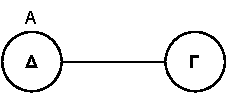
\includegraphics[scale = 0.9]{img/k1.pdf}
  \end{figure}
  Dove si hanno due nodi, $\Gamma$ e $\Delta$, e in cui se una FBF non viene
  indicata per un nodo significa che è falsa, mentre se viene segnata, come $A$
  per $\Delta$, significa che è vera.\\
  Possiamo leggere il modello come: ``in $\Gamma$ sono false tutte le formule
  ben formate, in $\Delta$ sono false tutte le formule ben formate escluso $A$
  che è vero''. Abbiamo quindi $\Delta\vDash A$ e $\Gamma\nvDash A$.\\
  Voglio sapere se:
  \[\Gamma\vDash A\lor\neg A\]
  Quindi mi serve che $\Gamma\vDash A$ oppure $\Gamma\vDash \neg A$. Ho che
  $\Gamma\nvDash A$ non avendo l'etichetta $A$. Studio ora $\Gamma\vDash \neg
  A$. Mi serve che:
  \[\Delta\nvDash A,\,\,\,\forall \Delta\in G \mbox{ t.c. } \Gamma R\Delta\]
  Ma so che $\Delta\vDash A$ e quindi anche $\Gamma\vDash \neg A$ non è vera. Ne
  segue che, non essendo vero né $\Gamma\vDash A$ né $\Gamma\vDash \neg A$:
  \[\Gamma\nvdash A\lor \neg A\]
  Avendo che la non dimostrabilità del terzo escluso, dimostrata coi tableaux,
  corrisponde alla non veridicità del terzo escluso, dimostrata ora coi modelli
  di Kripke, avendo un modello che rende falsa la formula, che è appunto un
  \textbf{contromodello} (che per di più questo è il modello di Kripke
  ``standard'' usato per il terzo escluso). \\
  Ipotizzando di essere in logica classica con un modello di Kripke ad un solo
  stato non potrei giungere a tale conclusione infatti il terzo escluso vale in
  logica classica. Non potrei prendere il modello a fatto ma ne prenderei uno
  con solo $\Gamma$ senza alcuna formula valida in $\Gamma$, verificando $A\lor
  \neg A$ in quanto in $\Gamma$ è verificato $\neg A$ non avendo altri nodi per
  la regola del $\neg$ di Kripke (come invece si ha in logica intuizionistica).
\end{esempio}
\begin{teorema}[Teorema di completezza e validità]
  La non dimostrabilità corrisponde alla non veridicità. In altri termini tutto
  ciò che si fa
  sintatticamente ha il suo corrispondente semantico per cui tutte le formule
  per cui esiste un tableau chiuso hanno un modello di Kripke che le rende vere
  e le formule che non hanno un tableau chiuso hanno un modello di Kripke che
  le rende false.
\end{teorema}
\begin{esempio}
  Vediamo se intuizionisticamente se:
  \[\Gamma\nvDash\neg\neg A\to A\]
  Sappiamo già che non ha un tableau chiuso. Usiamo lo stesso modello
  dell'esempio precedente:
  \begin{figure}[H]
    \centering
    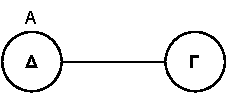
\includegraphics[scale = 0.9]{img/k1.pdf}
  \end{figure}
  Mi serve che:
  \[\Delta\nvDash \neg\neg A\mbox{ \textbf{o} }\Delta\vDash A,\,\,\,\forall
    \Delta\in G \mbox{ t.c. } \Gamma R\Delta\]
  Ma $\Delta\vDash A$ in quanto $A$ non vale in $\Gamma$ e $R$ è
  riflessiva, $\Gamma\nvDash A$. Ragiono ora su $\Delta\nvDash \neg\neg A$. Si
  ha però che $\Gamma\vDash \neg\neg A$, esistendo un $\Delta$ che rende vero
  $A$ (facendo i passaggi con la doppia negazione si arriva a voler cercare
  questo, devo avere che $\Gamma\nvDash\neg A$ e quindi che esiste almeno un
  $\Delta$ che verifica $A$), e quindi abbiamo dimostrato che: 
  \[\Gamma\nvDash\neg\neg A\to A\]
  Avendo un contro modello che verifica l'antecedente e non il conseguente
  dell'implicazione. 
\end{esempio}
\begin{esempio}
  Dimostriamo che intuizionisticamente:
  \[\Gamma\nvDash \neg\neg (A\lor B)\to \neg\neg A\lor \neg \neg B\]
  Il tableau di questa formula non è chiuso.\\
  Vediamo che esiste un contromodello (le due rappresentazioni sono
  equivalenti(???)):  
  \begin{figure}[H]
    \centering
    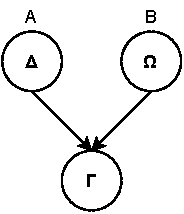
\includegraphics[scale = 0.9]{img/k2.pdf}
    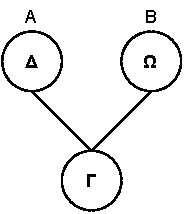
\includegraphics[scale = 0.9]{img/k3.pdf}
  \end{figure}
  Si ha quindi che $\Gamma$ è in relazione $R$ con se stesso, con $\Delta$, che
  a sua volta è in relazione solo con se stessa, e con $\Omega$, che è in
  relazione solo con se stessa. \\
  Partiamo con $\Gamma\vDash \neg\neg (A\lor B)$ che significa che esiste un
  nodo accessibile da $\Gamma$ in cui $A\lor B$ è vera. Questo è vero perché in
  $\Delta\vDash A$ e $\Omega\vDash B$ (ne basta uno dei due).\\
  Ora devo dimostrare che $\Gamma\nvDash\neg\neg A\lor \neg \neg B$ per avere
  che è un contromodello. Devo quindi avere che $\Gamma\nvDash \neg\neg A$ e
  $\Gamma\nvDash \neg\neg B$ in tutti i nodi accessibili da $\Gamma$. E vedo che
  in $\Delta$ non vale $B$ e in $\Omega$ non vale $A$, avendo quindi trovato il
  contromodello non potendo valere l'implicazione.
\end{esempio}
\subsection{Deduzione Naturale}
Introduciamo ora un nuovo calcolo, quello della \textbf{deduzione naturale},
introdotto da Gentzen negli anni '30 e perfezionato da Prawitz (perfezionamento
che tratteremo).\\
La deduzione naturale è un calcolo che è funzionale alla logica classica, alla
logica intuizionistica e alla logica minimale, con semplici variazioni nell'uso
delle regole.\\
La deduzione naturale è un calcolo la cui nozione di dimostrazione è molto
diversa dal calcolo a tableaux, che è un calcolo per refutazione (ovvero quando
vogliamo dimostrare una formula la segniamo $F$ e cerchiamo di ottenere una
configurazione chiusa ovvero una contraddizione), essendo quindi un calcolo
\textbf{indiretto e goal-oriented} ma che non permette di vedere come è fatta la
costruzione di una certa formula ma che dimostra che averla segnata $F$ porta ad
avere un tableau chiuso. Di contro la deduzione naturale utilizza, per
dimostrare una formula, un metodo diretto che, a partire da certe assunzioni,
costruisce la formula. Quindi l'ultimo passo di una dimostrazione in deduzione
naturale è la formula che si vuole dimostrare. \\
Con la scrittura
\[\bfrac{\pi}{A}\]
Diciamo che si è dimostrata la formula $A$ attraverso $\pi$, dove $\pi$ è un
insieme finito di passi, con eventuali assunzioni e applicazioni delle regole
della deduzione naturale.\\
Dire che $A$ è dimostrabile:
\[\vdash\bfrac{\pi}{A}\]
Significa dire che esiste una sequenza finita di applicazioni di regole e
assunzioni $\pi$ che termina con $A$ e quindi, non avendo alcuna formula a
sinistra di $\vdash$ si ha che la dimostrazione di $A$ non dipende da alcuna
formula e che in $\pi$ le eventuali assunzioni verranno chiuse, quindi sparendo,
rispetto alla deduzione di $A$ nei vari passi. Quindi $\vdash\bfrac{\pi}{A}$ è
il \textbf{frame} nel quale ci si muoverà.\\
La deduzione naturale comprende:
\begin{itemize}
  \item le \textbf{regole di introduzione}
  \item le \textbf{regole di eliminazione}
\end{itemize}
Date $A,B\in FBF$ si hanno:
\begin{table}[H]
  \Large
  \centering
  \begin{tabular}{c||c|c}
    connettivo& introduzione & eliminazione\\
    \hline
    \hline
    $\land$ & $\frac{A,B}{A\land B}i\land$&$\frac{A\land B}{A}e\land$
                                            $\frac{A\land B}{B}e\land$\\
    \hline
    $\lor$ &$\frac{A}{A\lor B}i\lor$
             $\frac{B}{A\lor B}i\lor$&$\frac{A\lor B,
                                       \bfrac{\bfrac{\cancel{A}}{\pi'}}{C},
                                       \bfrac{\bfrac{\cancel{B}}{\pi''}}{C}}{C}
                                       e\lor$\\
    \hline
    $\to$ & $\frac{\bfrac{\cancel{A}}
            {\bfrac{\pi}{B}}}{A\to B}i\to$ & $\frac{A,A\to B}{B}e\to$\\
    \hline
  \end{tabular}
\end{table}
Per l'eliminazione dell'or si ha che Prawitz ottiene questo risultato facendo:
\[\bfrac{\bfrac{A}{\pi'}}{C}\mbox{ e }\bfrac{\bfrac{B}{\pi''}}{C}\]
Ovvero se esiste una dimostrazione di $C$ che dipende solo da $A$ o $B$ sono
libero di dedurre $C$ tramite eliminazione dell'or \textbf{dimenticando},
specificata con $\cancel{A}$ e $\cancel{B}$, le
assunzioni che ho separatemene di $A$ e di $B$, avendo $A\lor B$ come
assunzione: 
\[\frac{A\lor B,\bfrac{\bfrac{\cancel{A}}{\pi'}}{C},
    \bfrac{\bfrac{\cancel{B}}{\pi''}}{C}}{C}e\lor\]
tengo solo in considerazione la dimostrazione di $A\lor B$, quindi la scrittura
corretta è, qualora non sia quindi un'assunzione:
\[\frac{\bfrac{\pi}{A\lor B},\bfrac{\bfrac{\cancel{A}}{\pi'}}{C},
    \bfrac{\bfrac{\cancel{B}}{\pi''}}{C}}{C}e\lor\]
$C$ è una nuova formula che non è necessariamente contenuta in $A$ o $B$. Se non
si riesce a trovare questa $C$ non si può fare l'eliminazione dell'or.\\
Per l'inserimento dell'implicazione si suppone di fare un'assunzione $A$. Se
dopo un numero finito di applicazioni di regole $\pi$ otteno $B$ allora posso
introdurre l'implicazione $A\to B$. Si dice che la regola ``scarica''
l'assunzione $A$ e quindi indichiamo $\cancel{A}$. Quando scrivo poi
l'implicazione ho comunque che la dimostrazione non dipende più da $A$ perché è
già compresa in $A\to B$.\\
La regole di eliminazione dell'implicazione è detta \textbf{modus ponens}.\\
In merito all'implicazione ho che se ho un conseguente posso anche derivare
un'implicazione con qualsiasi antecedente, senza scaricare nulla:
\begin{gather*}
  \frac{^1\cancel{A},^2B}{}i\land\\
  \frac{A\land B}\land\\
  \frac{B}{A\to B}i\to\mbox{scaricando solo 1}
\end{gather*}
È quindi una semplificazione della regola di introduzione dell'implicazione.\\
\textbf{Queste regole sono valide sia per la logica classica che per quella
  intuizionistica che per quella modale.}\\
Dopo le regole dei tre connettivi binari abbiamo quelle per la costante del
\textit{falso}:
\begin{table}[H]
  \Large
  \centering
  \begin{tabular}{c||c|c}
    & introduzione & eliminazione\\
    \hline
    \hline
    $\bot$ & $\frac{A,\neg A}{\bot}i\bot$& $\frac{\bot}{B}e\bot$\\
    \hline
  \end{tabular}
\end{table}
L'eliminazione del falso mi ricorda che dal falso segue qualsiasi cosa. \\
\textbf{La regola dell'eliminazione del $\bot$ non si può usare in logica
  minimale}. \\
Possiamo quindi passare al connettivo unario della negazione:
\begin{table}[H]
  \Large
  \centering
  \begin{tabular}{c||c|c}
    & introduzione & eliminazione\\
    \hline
    \hline
    $\neg$ & $\frac{\bfrac{\bfrac{\cancel{A}}{\pi}}
             {\bot}}{\neg A}i\neg$& $\frac{\bfrac{\bfrac{\cancel{\neg A}}{\pi}}
             {\bot}}{ A}e\neg$\\
    \hline
  \end{tabular}
\end{table}
\textbf{La regola dell'introduzione del $\neg$ non si può usare in logica
  minimale}.\\
\textbf{La regola dell'eliminazione del $\neg$ non si può usare in logica
  intuizionistica}.\\
Questo calcolo, per $\neg$, è ``sovrabbondante'' rispetto alle regole in quanto
potrei riscrivere $\neg A$ come $A\to\bot$ ed eliminare le regole del
$\neg$. Per di più con questa implicazione Prawitz ha chiuso un problema aperto
che Gentzen, usando solo il $\neg$, non era riuscito a chiudere, ovvero il
\textbf{teorema di normalizzazione in logica intuizionistica con il calcolo
  della deduzione naturale}, dimostrando che tutte le dimostrazioni in deduzione
naturale possono essere normalizzate, ovvero ridotte ad una forma
\textit{normale}. \\
\textit{Gentzen ha chiamato questo calcolo deduzione naturale perché era
  fermamente convinto che questo fosse il modo di ragionare in matematica in
  modo ``naturale''.}\\
Vediamo quindi come costruire dimostrazioni in deduzione naturale, in una certa
logica. Anche in questo caso sintassi e semantica devono essere 
coerenti, ovvero formule valide nella logica data devono essere
dimostrabili con la deduzione naturale e formule non valide non devono essere
dimostrabili in nessun modo.\\
La prima difficoltà riguarda il come far partire la dimostrazione e questo è il
motivo per cui tutti i prover automatici per la deduzione naturale sono stati un
fallimento (mentre coi tableaux sappiamo sempre da dove partire).\\
\begin{definizione}
  Una dimostrazione $\vdash A$ di una formula $A$, in deduzione naturale, è una
  sequenza finita di applicazioni di regole, $\pi$, della deduzione naturale che
  termina con la formula $A$ e in cui eventuali assunzioni devono essere state
  tutte ``scaricate'', essendo quindi chiusa rispetto alle assunzioni:
  \[\bfrac{\pi}{A}\]
  Se $A$ è dimostrabile da un insieme di formule $A_1,\ldots A_n$ di premesse
  allora in $\pi$ possono rimanere assunte $A_1,\ldots A_n$. Questo si indica
  con:
  \[A_1,\ldots A_n\vdash A\]
\end{definizione}
Vediamo qualche esempio.
\begin{esempio}
  Il primo esempio è quello del terzo escluso in logica classica (vedendo anche
  perché non vale in logica intuizionistica).\\
  Con $\vdash_{CL}$ indichiamo che una cosa è dimostrabile in logica
  classica. Vogliamo quindi dimostrare che:
  \[\vdash_{CL}A\lor \neg A\]
  Numeriamo le assunzioni, per poter indicare accanto alla regola che scarica
  l'assunzione il suo numero:
  \begin{enumerate}
    \item $A$
    \item $\neg(A\lor \neg A)$
  \end{enumerate}
  Procedo quindi:
  \[\frac{^1A}{A\lor \neg A}i\lor\]
  Potremmo pensare di aver finito, avendo ottenuto la formula, ma non è
  così. Dobbiamo infatti scaricare l'assunzione $A$. Assumo quindi un'altra
  assunzione, la 2 e procedo:
  \[\frac{^2\neg(A\lor \neg A), A\lor \neg A}{\bot}i\bot\]
  Ma dal falso posso dire che segue qualsiasi cosa in logica classica e quindi,
  iniziando a scaricare l'assunzione 1:
  \[\frac{\bot}{\neg A}i\neg\]
  Quindi, nel complesso ho:
  % {\Large{\[\frac{^1\cancel{A}}{\frac{^2\neg(A\lor \neg A), A\lor \neg
  %   A}{\frac{\bot}{\neg A}i\neg}i\bot}i\lor\]}}
  \begin{gather*}
    \frac{^1\cancel{A}}{}i\lor\\
    \frac{^2\neg(A\lor \neg A), A\lor \neg A}{}i\bot\\
    \frac{\bot}{\neg A}i\neg
  \end{gather*}
  Devo ancora scaricare la 2. Continuo:
  \[\frac{\neg A}{A\lor \neg A}i\lor\]
  Ma devo ancora scaricare la 2. Assumo quindi nuovamente la 2:
  \[\frac{^2\neg(A\lor \neg A), A\lor \neg A}{\bot}i\bot\]
  E quindi:
  \[\frac{\bot}{\neg \neg(A\lor \neg A)}i\neg\]
  che scarica 2, avendo complessivamente:
  % {\Large{\[\frac{^1\cancel{A}}{\frac{^2\cancel{\neg(A\lor \neg A)}, A\lor \neg
  %           A}{\frac{\bot}{\frac{\neg A}{\frac{^2\cancel{\neg(A\lor \neg A)},
  %                 A\lor \neg A}{\frac{\bot}{\neg \neg(A\lor \neg
  %                   A)}i\neg}i\bot}i\lor}i\neg}i\bot}i\lor\]} }
  \begin{gather*}
    \frac{^1\cancel{A}}{}i\lor\\
    \frac{^2\cancel{\neg(A\lor \neg A)}, A\lor \neg A}{}i\bot\\
    \frac{\bot}{}i\neg\\
    \frac{\neg A}{}i\lor\\
    \frac{^2\cancel{\neg(A\lor \neg A)}, A\lor \neg A}{}i\bot\\
    \frac{\bot}{\neg \neg(A\lor \neg A)}i\neg
  \end{gather*}

 % \end{equation*}
  Ma sono arrivato alla doppia negazione del principio del terzo escluso e non
  al terzo escluso. Finora ho usato solo regole valide anche in logica
  intuizionistica, che indico con $INT$ e quindi la doppia negazione del terzo
  escluso è dimostrabile 
  in logica intuizionistica, avendo scaricato tutte le assunzioni e avendo usato
  regole valide in quella logica:
  \[\vdash_{INT}\neg \neg(A\lor \neg A)\]
  Ovviamente la doppia negazione del terzo
  escluso vale anche in logica classica per lo stesso ragionamento.\\
  Voglio però arrivare al terzo escluso in logica classica. Per scaricare la 2
  posso fare eliminazione del \textit{false} (che non vale in logica
  intuizionistica ma solo in logica classica):
  \[\frac{\bot}{A\lor \neg A}e\bot\]
  che consuma la 2:
  \begin{gather*}
    \frac{^1\cancel{A}}{}i\lor\\
    \frac{^2\cancel{\neg(A\lor \neg A)}, A\lor \neg A}{}i\bot\\
    \frac{\bot}{}i\neg\\
    \frac{\neg A}{}i\lor\\
    \frac{^2\cancel{\neg(A\lor \neg A)}, A\lor \neg A}{}i\bot\\
    \frac{\bot}{A\lor \neg A}e\bot
  \end{gather*}
  arrivando quindi a:
  \[\vdash_{CL}A\lor \neg A\]
  Che non è dimostrabile in logica intuizionistica (come già si sapeva).
\end{esempio}
\begin{esempio}
  Vediamo una delle formule di De Morgan:
  \[\vdash_{INT}\neg(A\lor B)\to \neg A\land \neg B\]
  Come assunzioni ho:
  \begin{enumerate}
    \item $\neg (A\lor B)$
    \item $A$
    \item $B$
  \end{enumerate}
  Parto dal basso, sapendo che vorrei ottenere:
  \[\frac{\neg A\land \neg B}{\neg(A\lor B)\to \neg A\land \neg B}i\to\mbox{
      (scaricando 1)}\]
  Vediamo i passaggi i passaggi ``risalendo'', procedendo, come si dice, ``per
  necessità'' (ricostruendo ogni volta ciò che mi serve risalendo nella
  dimostrazione, ricostruendola a ritroso): 
  \begin{gather*}
    \frac{^2\cancel{A}}{}i\lor \mbox{, } \frac{^3\cancel{B}}{}i\lor\\
    \frac{A\lor B, ^1\cancel{\neg (A\lor B)}}{}i\bot \mbox{, } \frac{A\lor
      B,^1\cancel{\neg (A\lor B)}}{}i\bot\\  
    \frac{\bot}{}i\neg \mbox{(scaricando 2), }\frac{\bot}{}i\neg\mbox{
      (scaricando 3)}\\ 
    \frac{\neg A, \neg B}{}i\land\\
    \frac{\neg A\land \neg B}{\neg(A\lor B)\to \neg A\land \neg B}i\to\mbox{
      (scaricando 1)}
  \end{gather*}
  Chiudendo la dimostrazione avendo scaricato tutto ed essendo arrivati alla
  formula voluta. L'unico passo ``strano'', era capire che $\neg A/B$ era in
  contraddizione con $A/B$, portando all'introduzione dell'or e poi del
  $\bot$.\\
  Vediamo un'altra dimostrazione della stessa:
  \[\vdash_{INT}\neg(A\lor B)\to \neg A\land \neg B\]
  Assumo:
  \begin{enumerate}
    \item $A$
    \item $\neg(A\lor B)$
    \item $B$
  \end{enumerate}
  Procediamo quindi con la dimostrazione:
  \begin{gather*}
    \mbox{Ho }\pi_1 =\\
    \frac{ ^1\cancel{A}}{}i\lor\\
    \frac{A\lor B, ^2\cancel{\neg(A\lor B)}}{}i\bot\\
    \frac{\bot}{\neg A}i\neg\mbox{(scaricando 1)}\\
    \mbox{rifaccio anche con B, avendo} \pi_2=\\
    \frac{ ^3\cancel{B}}{}i\lor\\
    \frac{A\lor B, ^2\cancel{\neg(A\lor B)}}{}i\bot\\
    \frac{\bot}{\neg B}i\neg\mbox{(scaricando 3)}\\
    \mbox{sono nella situazione}\\
    \frac{\pi_1, p_2}{}i\land\\
    \frac{\neg A \land \neg B}{\neg(A\lor B)\to \neg A\land \neg
      B}i\to\mbox{(scaricando 2)}  
  \end{gather*}
  (i passaggi di $\pi_1$ e $\pi_2$ li avrei potuti scrivere uno accanto
  all'altro). \\
  Quindi, avendo usato solo regole valide per la logica intuizionistica:
  \[\vdash_{INT}\neg(A\lor B)\to \neg A\land \neg B\]
  Passiamo alla dimostrazione della conversa:
 \[\vdash_{INT}\neg A\land \neg B\to\neg(A\lor B)\]
 Sappiamo già che il tableau non chiude.\\
 Assumo:
 \begin{enumerate}
   \item $\neg A\land \neg B$
   \item $A\lor B$
   \item $A$
   \item $B$
 \end{enumerate}
 Procediamo quindi con la dimostrazione:
 \begin{gather*}
   \frac{^1\cancel{1\neg A\land \neg B}}{}e\land\mbox{, }\frac{^1\cancel{1\neg
         A\land \neg B}}{}e\land\\ 
   \frac{\neg A, ^3 \cancel{A}}{}i\bot\mbox{, }\frac{\neg B,
     ^4\cancel{B}}{}i\bot\\  
   \frac{\bot,\bot,^2\cancel{A\lor B}}{}e\lor\mbox{(scaricando 3 e 4)}\\
   \frac{\bot}{}i\neg\mbox{(scaricando 2)}\\
   \frac{\neg(a\lor B)}{\neg A\land \neg B\to\neg(A\lor B)}i\to\mbox{(scaricando
     1)} 
 \end{gather*}
 Ho quindi dimostrato, nel complesso, un'equivalenza avendo entrambi i versi
 dell'implicazione (e per entrambi i versi si ha un tableau chiuso), sia in
 logica classica che intuizionistica.  
\end{esempio}
\begin{esempio}
  Proviamo a dimostrare l'altra formula di De Morgan:
  \[\vdash_{INT}\neg(A\land B)\to \neg A\lor \neg B\]
  Il tableau della formula non chiude quindi arriveremo a dire che:
  \[\nvdash_{INT}\neg(A\land B)\to \neg A\lor \neg B\]
  Siano date le seguenti assunzioni:
  \begin{enumerate}
    \item $A$
    \item $B$
    \item $\neg(A\land B)$
  \end{enumerate}
  Procediamo quindi con la dimostrazione:
  \begin{gather*}
    \frac{^1\cancel{A},^2B}{}i\land\\
    \frac{A\land B, ^3\cancel{\neg(A\land B)}}{}i,\bot\\
    \frac{\bot}{}i\neg\mbox{(scaricando 1)}\\
    \frac{\neg A}{}i\lor\\
    \frac{\neg A \lor \neg B}{}i\to\mbox{(scaricando 3)}\\ 
    \frac{\neg(A\land B)\to\neg A\lor \neg B}{}
  \end{gather*}
  Ma non si è scaricato $B$ e quindi non è una dimostrazione, né classica né
  intuizionistica.\\
  Vediamo se la conversa vale intuizionisticamente:
  \[\vdash_{INT}\neg A\lor \neg B\to\neg(A\land B)\]
  Assumo:
  \begin{enumerate}
    \item $\neg A\lor \neg B$, ovvero assumo l'antecedente
    \item $\neg A$
    \item $\neg B$
    \item $A\land B$
  \end{enumerate}
 Procediamo quindi con la dimostrazione:
 \begin{gather*}
    \frac{ ^4\cancel{A\land B}}{}e\land\mbox{, }
    \frac{ ^4\cancel{A\land B}}{}e\land\\
    \frac{A, ^2\cancel{\neg A}}{}i\bot\mbox{, }
    \frac{B,^3\cancel{\neg B}}{}i\bot\\
    \frac{\bot, ^1\cancel{\neg A\lor \neg B}}{}e\lor\mbox{(scaricando 2 e 3)}\\
    \frac{\bot}{}i\neg\mbox{(scaricando 4)}\\
    \frac{\neg (A\land B)}{\neg A\lor \neg B\to\neg(A\land
      B)}i\to\mbox{(scaricando 1)} 
  \end{gather*}
  Quindi, avendo usato solo regole valide per la logica intuizionistica:
  \[\vdash_{INT}\neg A\lor \neg B\to\neg(A\land B)\]
  Quindi ``mezza'' De Morgan vale in logica intuizionistica.
\end{esempio}
\noindent
\textbf{Durante la lezione 6, parte 2, altri esempi di dimostrazione}:
\begin{itemize}
  \item $\vdash_{INT}(A\to\neg B)\to(B\to \neg A)$
  \item $\vdash_{INT}(\neg A\lor\neg B)\to(B\to \neg A)$
  \item $\vdash_{INT}(A\to(B\to C))\to(B\to(A\to C)$, detta \textbf{scambio
    degli antecedenti}  
  \item $\nvdash_{INT} ((A\to B)\to A)\to A$, detta \textbf{legge di Peirce},
  che vale solo in logica classica
  \item $\nvdash_{INT}(A\to B)\iff(\neg B\to \neg A)$, detta \textbf{legge di
    contrapposizione}, che ricorda il\textbf{ teorema di deduzione della logica
    classica} che legava dimostrabilità e implicazione, avendo a livello
  proposizionale che se con ipotesi $A$ dimostro $B$, $A\vdash B$ allora $A\to
  B$. Classicamente si ha anche che $\vdash \neg B\to \neg A$ se $A\vdash B$ e
  si noti che è il procedimento di una \textit{dimostrazione per assurdo},
  secondo la logica classica. Vale in logica classica ma il $\gets$ non vale in
  logica intuizionistica. \textbf{Non posso dimostrare direttamente per assurdo
    in logica intuizionistica} ma si usano dei ``meta-sistemi''
  \item $\vdash_{INT}((((A\to B)\to A)\to A)\to B)\to B$
\end{itemize}
\textbf{Se la formula è un'implicazione si assume spesso l'antecedente che poi
  si scarica all'ultimo passo.} \\
\textbf{Non si hanno comunque strategie deterministiche.}\\
Si è notato come non ci sia un metodo preciso per ottenere la strategia e per di
più la strategia non è unica potenzialmente. Nel primo esempio si parte
dall'alto, nel secondo dal basso.\\
Per capire se esiste una dimostrazione faccio prima la prova coi tableaux, che
se chiude mi garantisce l'esistenza di una dimostrazione.\\
L'idea di partire a dimostrare sapendo a quali connettivi bisogna arrivare si
adatta molto bene anche al \textbf{calcolo dei sequenti} di Gentzen (sono un
calcolo diretto), dove si
parte sempre dal basso, risalendo ``per necessità'', fino ad arrivare agli
assiomi caratteristici della logica in uso e del calcolo dei sequenti. Si hanno
meccanismi di traduzione da tableaux intuizionistici a sequenti e da sequenti a
deduzione logica (\textit{argomento non approfondito}). I sequenti sono
``mediani'' nel paradigma del goal-oriented. \\
Anche in deduzione naturale, in modo analogo alla matematica, si possono usare i
\textbf{lemmi}.
\begin{esempio}
  Dimostriamo:
  \[\vdash_{INT}\neg\neg (A\land B)\to \neg\neg A\land \neg \neg B\]
  Si assume:
  \begin{enumerate}
    \item $\neg A$
    \item $\neg\neg(A\land B)$
    \item $\neg B$
  \end{enumerate}
  Di ha quindi la dimostrazione:
  \begin{gather*}
    \frac{^1 \cancel{\neg A}}{}i\lor \mbox{, }
    \frac{^3 \cancel{\neg B}}{}i\lor\\
    \frac{\neg A\lor \neg B}{\rule{49pt}{0.4pt}}\mbox{regola derivata, }
    \frac{\neg A\lor \neg B}{\rule{49pt}{0.4pt}}\mbox{regola derivata}\\
    \frac{\neg (A\land B),^2\cancel{\neg\neg(A\land B)}}{}i\bot\mbox{, }
    \frac{\neg  (A\land B),^2\cancel{\neg\neg(A\land B)}}{}i\bot\\ 
    \frac{\bot}{}i\neg\mbox{(scaricando 1), }
    \frac{\bot}{}i\neg\mbox{(scaricando 3)}\\ 
    \frac{\neg\neg A, \neg\neg B}{}i\land\\
    \frac{\neg\neg A\land \neg\neg B}{\neg\neg (A\land B)\to \neg\neg a\land
      \neg \neg B}i\to \mbox{(scaricando 2)}
  \end{gather*}
  con la doppia barra indico una regola derivata da un precedente lemma (nel
  nostro caso dalla legge/teorema di De Morgan) che quindi chiamiamo lemma di De
  Morgan, non dovendo quindi dimostrare nuovamente la cosa, riducendo la
  ``complessità'' della dimostrazione.
\end{esempio}
Comunque non si hanno strategie deterministiche per iniziare una dimostrazione,
si hanno comunque suggerimenti in base alla formula, ad esempio se ho una cosa
del tipo $A\to B$ si parte spesso, ma non sempre, assumendo $A$ per poi cercare
di scaricarla. Bisogna sempre prima guardare bene la formula che si deve
dimostrare, ragionando su sottoformule etc$\ldots$
\subsection{Ottimizzazione dei Tableaux}
Parliamo ora di \textbf{ottimizzazione dei tableaux intuizionistici}.
\begin{esempio}
  Riprendiamo il tableau di Fitting per la doppia negazione del terzo escluso:
  \[F\neg \neg (A\lor \neg A)\]
  che ricordiamo dimostrabile in logica intuizionistica per il teorema di
  Kolmogorov-Glivenko. \\
  Riprendiamo il tableau di Fitting:
  \begin{gather*}
    \frac{F\neg \neg (A\lor \neg A)}{}\\
    \frac{T\neg(A\lor \neg A)}{}\\
    \frac{FA\lor \neg A}{}\\
    \frac{FA,F\neg A}{TA}
  \end{gather*}
  Che sembra non chiudere. \\
  Si ricorda però che, sempre Fitting, risolve la questione ripetendo una
  formula: 
  \begin{gather*}
    \frac{F\neg \neg (A\lor \neg A)}{}\\
    \frac{T\neg(A\lor \neg A)}{}\\
    \frac{FA\lor \neg A, T\neg(A\lor \neg A)}{}\\
    \frac{FA,F\neg A,T\neg(A\lor \neg A)}{}\\
    \frac{TA,T\neg(A\lor \neg A)}{}\\
    \frac{TA, FA\lor \neg A}{TA, FA, F\neg A}
  \end{gather*}
  che chiude.\\
  Si è usato il fatto che si è usata, come regola per il $T$ di $\neg$:
  \[\frac{S, T\neg A}{S, FA, T\neg A}\]
\end{esempio}
Nell'esempio ci si è rifatti al concetto di \textbf{realizzabilità}.
\begin{definizione}
  Preso un nodo $\Gamma$ di un modello di Kripke per la logica intuizionistica
  diremo che $\Gamma$ \textbf{realizza} $TA$ sse $\Gamma$ \textup{forza} $A$,
  ovvero sse: 
  \[\Gamma\vDash A\]
  Inoltre si ha che $\Gamma$ \textbf{realizza} $FA$ sse in $\Gamma$ \textbf{non
    è vera} $A$, ovvero sse:
  \[\Gamma\nvDash A\]
  Abbiamo quindi legato il segno $T/F$ al \textbf{forcing intuizionista}. Le
  regole devono quindi mantenere la realizzabilità.
\end{definizione}
Vediamo, sempre pensando all'esempio, cosa significhi mantenere la
realizzabilità parlando di $T\neg A$. Si ha che, intuizionisticamente:
\[\Gamma\vDash \neg A\]
Ma nell'intuizionismo significa che:
\[\forall\Delta \mbox{ t.c }\Gamma R \Delta, \Delta\nvDash A\]
Se diciamo che una formula realizzata prima di applicare una regola deve essere
realizzata anche dopo tale applicazione si ha che, avendo:
\[\frac{S, T\neg A}{S, FA, T\neg A}\]
$FA$ può essere eliminata, quindi restringendo $S$ a $S_C$ non è più garantito
che sia realizzato $FA$ ovvero che sia forzata $A$. Dato che questo deve
avvenire $\forall\Delta$ mi ``porto dietro'' $T\neg A$ in modo che in ogni punto
del tableau sia realizzabile la formula $\neg A$ (ma questo succede solo se
ripeto il $T$).\\
Non sempre bisogna ripetere la $T$, ad esempio:
\[\frac{S, T(A\land B)}{S, TA, TB}\]
che passando da una $T$ a due $T$ non crea problemi anche se restringo a
$S_T$, avendo un $\Gamma$ che realizza $TA$ e $TB$ allora ho che forza $A\land
B$.\\
Vale lo stesso discorso anche avendo:    
\[\frac{S, T(A\lor B)}{S, TA/S, TB}\]
garantendo o da un alto o dall'altro la realizzabilità di $A\lor B$. Infatti se
è 
realizzato $TA$ ho un $\Gamma$ che forza $A$ e che automaticamente forza $A\lor
B$. Viceversa con $TB$ ho un $\Gamma$ che forza $B$ e che automaticamente forza
$A\lor B$.\\
Abbiamo un'altra regola che obbliga a ripete:
\[\frac{S, T(A\to B)}{S, FA, T(A\to B)/S, TB}\]
Dove, avendo che $FA$ può essere ``tagliato'' da una restrizione $S_T$ nel primo
branch, conservo anche la formula (non avendo $F$ nel secondo branch non devo
ripetere). \\
Vediamo un calcolo che, ``modulo backtracking'', non necessiterà della
ripetizione delle formule, avendo già tutta la sua semantica all'interno del
calcolo. Si parla quindi di \textbf{semantic tableau}, avendo che i tableaux
``mimano'' la semantica della logica di riferimento. Più semantica
incorporariamo nelle regole stesse e migliore sarà il calcolo dal punto di vista
dell'efficienza.\\
Quanto detto viene bene con il $T$ di $\neg$.\\
Aggiungiamo a $T$ e $F$ il segno $F_C$ che significa \textbf{falso certo}:
\begin{table}[H]
  %\large
  \centering
  \begin{tabular}{c||c|c|c}
    & {\small{$T$-regola}}& {\small{$F$-regola}} & {\small{$F_C$-regola}}\\
    \hline
    \hline
    $\land$ & $T\land=\frac{S,T(A\land B)}{S,TA,TB}$&
              $F\land=\frac{S,F(A\land B)}{S,FA/S,FB}$&
              $F_C\land=\frac{S,F_C(A\land B)}{S_C,F_CA/S_C,F_CB}$\\ 
    \hline
    $\lor$ & $T\lor=\frac{S,T(A\lor B)}{S,TA/S,TB}$&
                        $F\lor=\frac{S,F(A\lor B)}{S,FA,FB}$&
                        $F_C\lor=\frac{S,F_C(A\lor B)}{S,F_CA,F_CB}$\\
    \hline
    $\to$ & $T\to=\frac{S,T(A\to B)}{S,FA, T(A\to B)/S,TB}$&
                        $F\to=\frac{S,F(A\to B)}{S_C,TA,FB}$&
                        $F_C\to=\frac{S,F_C(A\to B)}{S_C,TA,F_CB}$\\
    \hline
    $\neg$ & $T\neg=\frac{S,T(\neg A)}{S,F_CA}$&
                        $F\neg=\frac{S,F(\neg A)}{S_C,TA}$&
                        $F_C\neg=\frac{S,F_C(\neg A)}{S_C,TA}$\\
    \hline
  \end{tabular}
\end{table}
Il nuovo segno è dato in quanto la semantica del $\neg$ ci dice che, avendo il
forcing di $\neg A$, $A$ deve rimanere falso in ogni nodo del modello di Kripke
e quindi è un falso che deve permanere sempre in tutto il tableau.\\
$S_C$ è definito come l'insieme $S$ meno l'insieme delle formule segnate con
$F$ (detto $FC_J$): 
\[S_C=S-\{FC_j\}\]
Notiamo, in prima istanza, come da formule $F_C$ otteniamo sempre formule $F_C$
o $T$, stabilizzando il tableau.\\
Nell'implicazione di $F_C$ notiamo ancora però la presenza di $TA$ che
porterebbe a fare lo stesso ragionamento di replicazione della formula
dell'implicazione ma questo è uno step successivo di ottimizzazione.\\
Un tableau in questo nuovo calcolo è chiuso secondo le regole dei normali
tableaux ma anche se ho $TA,F_CA$.
\begin{esempio}
  Riprendiamo la doppia negazione del terzo escluso con questo nuovo calcolo:
  \begin{gather*}
    \frac{F\neg \neg (A\lor \neg A)}{}\\
    \frac{T\neg(A\lor \neg A)}{}\\
    \frac{F_C (A\lor\neg A)}{}\\
    \frac{F_C A, F_C\neg A}{}\\
    \frac{F_C A, TA}{}
  \end{gather*}
  e quindi il tableau è chiuso, anche senza aver ripetuto il $T\neg$.
\end{esempio}
\textbf{$F_C$ è stato proposto da Moscato a Fitting ed è stato accolto nello
  studio dell'intuizionismo}.\\
Si è quindi incorporato più semantica nel calcolo infatti:
\[\Gamma\vDash F_CA \iff \Gamma\vDash \neg A\]
avendo che la semantica del $\neg$ viene incorporata dal segno $F_C$, avendo che
$\Gamma$ realizza $F_C A$ sse realizza $\neg A$. Abbiamo fatto quindi un primo
step di ottimizzazione.\\
Dal punto di vista del ``proof teoretico'' il segno $F_C$ riesce a evitare
duplicazioni della formula $\neg A$, a livello intuizionista, che sarebbero
sempre necessarie per chiudere il tableau.
\begin{esempio}
  Ripariamo dalla doppia negazione del terzo escluso:
  \[\neg\neg(A\lor \neg A)\]
  Si ha, con il nuovo calcolo:
  \begin{gather*}
    \frac{F\neg\neg(A\lor \neg A)}{}\\
    \frac{T\neg (A\lor \neg A)}{}\\
    \frac{F_c(A\lor\neg A)}{}\\
    \frac{F_C A, F_C\neg A}{F_C A, TA}
  \end{gather*}
  Avendo che il tableau chiude (senza il ragionamento di Fitting di ripetere le
  formule).
\end{esempio}
Il discorso può essere generalizzato dicendo che, ogni volta che si vuole
applicare il teorema di Kolmogorov-Glivenko, ragionando come Fitting avrò sempre
bisogno di ripetere formule, avendo in partenza una doppia negazione (dovendo
fare comunque un $F\neg$ e un $T\neg$ come prime mosse, se non uso
$F_C$). Quindi, avendo una formula valida classicamente, per dimostrare
intuizionisticamente la doppia negazione, posso usare $F_C$ evitando la
ripetizione di formule, a meno di avere poi nella formula dei $T\to$. Si ha
quindi un \textbf{trattamento ottimale} del $T\neg$ ma manca quello di
$T\to$. \\
Moscato, coi vari collaboratori, ha lavorato anni per trovare una
soluzione soddisfacente, quindi un calcolo corretto e completo, che rimuovesse
anche la ripetizione del $T\to$. Si sono quindi chiesti se, a livello
proposizionale, esistesse una soluzione al problema. Si arriverà a dire che c'è
una soluzione a livello proposizionale ma non a livello predicativo (il
$T\forall$ richiede sempre e comunque la ripetizione) e
nemmeno a livello di logica classica (lato predicativo si ha ripetizione sia per
$T\forall$ che per $T\exists$). Nella logica classica, lato proposizionale, vale
quindi la regola di Chruch-Rosser e quindi non sarà mai necessario ripetere una
formula mentre in logica intuizionistica questo non vale e quindi bisogna
pensare a delle strategie per evitarlo. Il calcolo puro di Fitting prevede per
forza ripetizioni per $\neg$ e $T\to$ ma in questo nuovo calcolo con $F_C$ ho
solo ripetizioni per $T\to$.\\ 
Presentiamo quindi un ulteriore calcolo che rimuova anche questa ripetizione.\\
Questo nuovo calcolo proviene da un'idea di Dyckhoff, che aveva ragionato sulla
deduzione naturale e sul calcolo dei sequenti di Gentzen. Dyckhoff aveva studiato
cosa succede a livello di deduzione naturale quando si assumono nuovamente certe
formule, costruendo un calcolo in cui non succede. Moscato e Miglioli, studiando
il lavoro di Dyckhoff, hanno cercato di applicare le stesse regole al calcolo a
tableaux ottimizzato. \\
L'idea è di studiare in modo approfondito come è fatto l'antecedente
dell'implicazione e non dare una sola regola per il $T\to$ ma dare tante regole
a seconda della forma dell'antecedente dell'implicazione.\\
Si va quindi ad analizzare la formula del tipo:
\[T\,\, A\to B\]
Si studia l'antecedente $A$. Si hanno quindi vari casi:
\begin{itemize}
  \item $A$ è atomica o negata, che indico con $AN$ (per dire $A$ e Negata)
  \item $A$ è una disgiunzione, quindi del tipo $A=C\lor D$
  \item $A$ è una congiunzione, quindi del tipo $A=C\land D$
  \item $A$ è un'implicazione, quindi del tipo $A\to B$
\end{itemize}
Si da quindi una regola ad hoc per ciascuna tipologia di antecedente. Si hanno
quindi quattro formule.\\
Facciamo qualche considerazione preliminare. In primis si nota come il calcolo
venga ancora più complicato, complicando il lavoro di un prover, anche se questo
è trascurabile dal punto di vista computazionale. Una seconda osservazione è che
non si riesce a trovare un modo per importare nel calcolo la semantica
dell'implicazione, come per il caso di $T\neg$, che importava la semantica della
negazione intuizionistica nel calcolo. Questa infatti è un'idea più
\textit{sintattica} e sostituisce una formula con un suo equivalente
intuizionista, che abbia nell'antecedente una complessità implicazionale sempre
più bassa, fino ad arrivare a formule atomiche o negate per poter applicare la
regola di base, avendo che la regola per le atomiche e le negate non prevede
ripetizioni di formule. Si ha quindi una ``trasformazione di formule''. Si
ottiene un calcolo privo di ripetizioni,\textit{ anche se può darsi che esista
  una soluzione più semantica e meno sintattica del problema di questo tipo di
  calcolo, magari cercando un nuovo segno ad hoc}. \\
Vediamo quindi queste 4 regole che sostituiscono la precedente regola per
$T\to$: 
\begin{table}[H]
  \Large
  \centering
  \begin{tabular}{c|c}
     Antecedente $Ant$ & $\mathbf{T\to}$\\
    \hline
    $Ant=A$ \textit{o} $Ant=\neg A$ & $\frac{S,TA\to B}{S,FA/S,TB}T\to AN$\\
    \hline
    $Ant=A\land B $ & $\frac{S,T(A\land B)\to C}{S,T(A\to(B\to C))}T\to \land$\\
    \hline
    $Ant=A\lor B$ & $\frac{S,T(A\lor B)\to C}{S,TA\to C, TB\to C}T\to \lor$\\
    \hline
    $Ant =A\to B$ & $\frac{S,T(A\to B)\to C}{S, FA\to B, TB\to C/S, TC}T\to \to$\\
    \hline
  \end{tabular}
\end{table}
Si nota che la complessità logica di $B$ non ha importanza. In tutti i casi si
ottengono complessità implicazionali minori, avendo antecedenti sempre meno
complessi logicamente nella risultante rispetto alla premessa.\\
Questo nuovo calcolo, con questa nuova regola per $T\to$ è \textbf{corretto,
  completo e senza ripetizioni}.\\
A livello di prover questo risultato permette di non dover creare liste
aggiuntive di formule da ripetere (considerando che Fitting nemmeno limitava la
cosa a $T\neg $ e $T\to$).
\begin{esempio}
  Studiamo:
  \[\vdash_{INT} ((\neg A\lor \neg \neg A)\to A)\to A\]
  \begin{gather*}
    \frac{F ((\neg A\lor \neg \neg A)\to A)\to A}{}F\to\\
    \frac{T(\neg A\lor \neg \neg A)\to A, FA}{}T\to\lor\\ 
    \frac{T\neg A\to A, T\neg\neg A\to A,FA}{}T\to AN\\
    \frac{T\neg A\to A, F\neg\neg A, FA/T\neg A\to A, TA,FA}{}F\neg\mbox{(chiude
      branch destro)}\\ 
    \frac{T\neg A\to A,T\neg A}{}T\neg\\
    \frac{T\neg A\to A,F_C A}{}T\to AN\\
    \frac{F\neg A, F_CA/TA,F_CA}{}F\neg\mbox{(chiude branch destro)}\\
    TA, F_CA
  \end{gather*}
  Avendo che il tableau chiude, senza ripetizioni.\\
  Si nota che avendo $T\neg A\to A, T\neg\neg A\to A,FA$ si osserva che è
  prodotto da un antecedente in $\lor$ con due negate. Si hanno quindi ora due
  antecedenti entrambi con due negate, sotto $T$, che mi riportano alla regola
  per il $T\to$ delle atomiche e delle negate.
\end{esempio}
Dimostreremo che questo calcolo è corretto e completo.\\
Il prover PITP è basato su questo calcolo con ulteriori strategie di
ottimizzazione. \\
Possiamo quindi vedere la dimostrazione del teorema di Kolmogorov-Glivenko, che
riscriviamo per comodità, tramite il calcolo a tableaux con $F_C$ e la non
ripetizione di $T\neg$ e $T\to$.
\begin{teorema}[Teorema di Kolmogorov-Glivenko]
  Se una formula $A$ è dimostrabile in logica classica allora e solo allora è
  dimostrabile in logica intuizionistica la doppia negazione di tale formula, a
  livello proposizionale. Formalmente si ha quindi:
  \[\vdash_{CL} A \iff \vdash_{INT}\neg\neg A\]
  Quindi tutte le tesi classiche sono dimostrabili, se doppiamente negate, in
  logica intuizionistica.
\end{teorema}
\begin{proof}
  Per fare la dimostrazione si introduce una nuova regola:
  \[\frac{S, TA\to B}{S,F_CA/S_C, TB}\overline{T\to}\]
  che chiamiamo appunto $T\to$ soprassegnato. Questa regola è corretta dal punto
  di vista del calcolo intuizionistica e possiamo usarla quando vogliamo. La sua
  peculiarità rispetto all'originale $T\to$ è che nel branch a sinistra ho $F_C
  A$ quindi non si avrà mai il taglio della stessa applicando regole
  intuizionistiche. Nel branch di destra si ha $TB$ che già non verrebbe mai
  tagliata ama, per correttezza e non per completezza, si restringe $S$ a
  $S_C$.\\
  Ricordiamo che la vecchia regola era, dove si ripeteva la formula a causa di
  $FA$ nel branch di sinistra e non si restringeva $S$ in quello di destra:
  \[\frac{S, TA\to B}{S,FA, TA\to B/S, TB}T\to\]
  La $\overline{T\to}$ è una versione corretta ma non completa di $T\to$. L'uso
  della prima quindi comporta un calcolo corretto ma non completo, mentre la
  seconda sia corretto che completo.\\
  Ora a noi basta avere una formula corretta, cosa che rende possibile il
  poterla applicare ogni volta che voglio.\\
  Parto quindi dal tableau intuizionista di $\neg\neg A$:
  \begin{gather*}
    \frac{F\neg\neg A}{}F\neg\\
    \frac{T\neg A}{F_C A}T\neg
  \end{gather*}
  Avendo che da questo momento in poi il tableau intuizionista diventa
  equivalente a quello classico, con solo i segni $T$ e $F_C$. Dobbiamo
  dimostrarlo per casi, a seconda della natura di $A$:
  \begin{itemize}
    \item $A$ è una formula atomica quindi se chiude classicamente $F_CA$ chiude
    anche intuizionisticamente
    \item $A$ è del tipo $B\lor C$, avendo che $F_C (B\lor C)$ produce/deduce
    $F_CB,F_CC$
    \item $A$ è del tipo $B\land C$, avendo che $F_C (B\land C)$ produce/deduce
    $F_CB/F_CC$
    \item $A$ è del tipo $\neg B$, avendo che $F_C \neg B$ produce/deduce $TB$
    \item $A$ è del tipo $B\to C$, avendo che $F_C (B\to C)$ produce/deduce
    $TB,F_CC$
  \end{itemize}
  Analizzo l'ultimo caso, avendo $TB,F_CC$. Questo è l'unico caso in cui potrei
  avere 
  ancora formule che vengono tagliate con le regole intuizionistiche, in caso di
  implicazione ma posso evitare la cosa. Infatti, se $TB$ fosse anch'essa
  un'implicazione, potrei usare il $\overline{T\to}$ e ottenere formule che non
  verranno mai tagliate dall'applicazione di regole intuizionistiche, avendo che
  il tableau classico e quello intuizionistico coincidono. Ne segue che se
  quello classico chiude allora chiude anche quello intuizionistico. Il trucco
  sta nel $F_CA$ nel branch sinistro del risultante della regola del
  $\overline{T\to}$, vale a dire rafforzare, scrivendo $F_C$ invece di $F$
  della'antecedente dell'implicazione e quindi ottenendo da una formula certa,
  $TA\to B$ due formule certe, una per branch, $F_CA$ e $TB$. Per questo logica
  classica e logica intuizionistica qui coincidono. Da un $T$ prodotto da un
  $F_C$ vengono quindi fuori solo formule certe con al nuova regola del
  $\overline{T\to}$. \\
  Si è arrivati a tutto questo discorso dicendo che bisogna chiudere il tableau
  per $F_CA$ e da quel punto in poi il tableau classico e quello intuizionista
  coincidono. Qualsiasi sia il tipo di $A$ (specificando nel caso
  dell'implicazione l'uso di $\overline{T\to}$) ottengo qualcosa che non è più
  ``tagliabile'' usando regole intuizionistiche e quindi, partendo da $F\neg
  \neg A$ e arrivando ad $F_CA$, anche qualora $A$ non sia atomica, arrivo ad
  un punto in cui le due logiche coincidono, \textbf{dimostrando il teorema},
  non avendo più regole intuizionistiche che possono tagliare.\\
  Si arriva a dire che, in questa situazione, l'$S$ classico e l'$S_C$
  intuizionistico coincidono.\\
  \emph{Essendo corretta la regola del $\overline{T\to}$ la posso usare
    nella dimostrazione del teorema. La regola non è completa perché esistono
    tesi intuizionistiche, dimostrabili intuizionisticamente, che non possono
    essere dimostrate usando la regola, che porterebbe ad un tableau che non
    chiude}. 
\end{proof}
\section{Logica Intuizionistica Predicativa}
Per parlare di logica predicativa intuizionistica abbiamo bisogno di specificare
il suo \textbf{alfabeto}, formato da:
\begin{enumerate}
  \item un insieme di \textbf{variabili individuali} che indichiamo con $x,y,z$
  etc$\ldots$ 
  \item un insieme di \textbf{costanti individuali}, detti anche
  \textbf{parametri} in certi contesti, che indichiamo con $a,b,c$ etc$\ldots$ 
  \item un insieme di \textbf{funzioni}, con la loro arietà (che ricordiamo
  essere  il numero degli argomenti o operandi che richiede), che indichiamo con
  $f,g,h$ etc$\ldots$  
  \item un insieme di \textbf{predicati}, con la loro arietà, che indichiamo con
  $P,Q,R$ etc$\ldots$  
  \item un insieme di \textbf{costanti logiche proposizionali} $\neg, \land,
  \lor, \to$
  \item un insieme di \textbf{quantificatori}, ovvero quello
  \textbf{esistenziale} $\exists$ e quello \textbf{universale} $\forall$ 
  \item un insieme di \textbf{simboli ausiliari}, come, ad esempio, ``(''  e
  ``)'' 
\end{enumerate}
Gli insiemi 1,5,6 e 7 sono generali per tutti i linguaggi intuizionistici. I
punti 2,3 e 4 sono detti \textbf{tipo di similarità} o \textbf{segnatura} dello
specifico linguaggio. Specificando quindi costanti individuali, funzioni e
predicati vado a specificare un particolare \textit{linguaggio del primo
  ordine}.\\
Rispetto all'alfabeto per il linguaggio del primo ordine della logica classica
non si riscontrano differenze con quello intuizionistico, i due alfabeti
coincidono (come del resto coincidevano anche gli alfabeti dei linguaggi
proposizionali). \\
Anche le altre definizioni, ovvero quelle di \textbf{termine} e
di \textbf{formula ben formata}, coincidono tra logica predicativa classica e
logica predicativa intuizionistica.
\begin{definizione}
  Definisco \textbf{termine}, in logica predicativa intuizionistica. Si ha che:
  \begin{enumerate}
    \item ogni costante individuale è un termine
    \item ogni variabile individuale è un termine
    \item se $t_1,\ldots, t_n$ sono termini e $f$ è una funzione di arietà $n$
    allora $f(t_1,\ldots, t_n)$ è un termine  
  \end{enumerate}
  Si ha che 1 e 2 sono i \textbf{casi base} mentre 3 è la \textbf{clausola
    induttiva}.
\end{definizione}
In un parallelo con il mondo della programmazione posso pensare ad un
\textbf{tipo}, ad esempio \texttt{int}. Ho che:
\begin{center}
  \texttt{x+1}
\end{center}
è una funzione binaria che somma ad una variabile $x$, che suppongo di tipo
\texttt{int}, una costante $1$, comunque di tipo \texttt{int}.\\
Si ha che, in programmazione, \texttt{x+1} è un'\textbf{espressione}, che è
appunto in programmazione il corrispettivo di \textbf{termine} nella logica.\\
Ogni linguaggio di programmazione ha una sua sintassi, definita tramite
\textbf{carte sintattiche}, esempio in figura \ref{fig:st}, usate per definire
una grammatica deterministica in un linguaggio di programmazione.
\begin{figure}
  \centering
  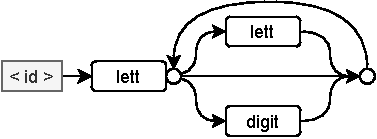
\includegraphics[scale = 1.3]{img/st.pdf}
  \caption{Esempio di carta sintattica in C, per un identificatore. Si legge
    ``un identificatore C 
    \textit{id} comincia sempre con una lettera alfabetica \textit{lett},
    seguita da una lettera alfabetica \textit{lett} o da una cifra
    \textit{digit}, il tutto iterato''. A esempio \texttt{A10} è un
    identificatore, \texttt{1AB} no.} 
  \label{fig:st}
\end{figure}
Quindi dal punto di vista della carta sintattica un'espressione è:
\begin{itemize}
  \item una costante
  \item una variabile
  \item un simbolo di funzione applicato a $n$ espressioni se il simbolo di
  funzione ha arietà $n$
\end{itemize}
Torniamo a parlare di logica predicativa.
\begin{definizione}
  Definiamo \textbf{termine chiuso} come un termine che non contiene variabili.
\end{definizione}
\begin{esempio}
  Ad esempio:
  \begin{itemize}
    \item $f(x,1)$, con $f$ di arietà 2, è un termine ma non è un termine
    chiuso, avendo $x$, che è una variabile, come argomento
    \item $g(4,7)$, con $g$ di arietà 2, è un termine ed è un termine chiuso,
    avendo solo costanti come argomento
    \item $g(f(x,2),4)$, con $g$ ed $f$ di arietà 2, è un termine, avendo una
    funzione ed una costante come parametri ed entrambi sono termini. Non è però
    un termine chiuso dato che $f(x,2)$ non è un termine chiuso
  \end{itemize}
\end{esempio}
\begin{definizione}
  Definiamo le \textbf{formule ben formate} del primo ordine. Si ha che:
  \begin{enumerate}
    \item se $P$ è un \textbf{predicato}, di arietà $n$ (cosa che potremmo
    indicare con $P^n$) e
    $t_1,\ldots, t_n$ sono \textbf{termini}, allora $P(t_1,\ldots, t_n)\in
    FBF$. $P(t_1,\ldots, t_n)$ è detta \textbf{formula atomica}
    \item se $\mathcal{A},\mathcal{B}\in FBF$ allora:
    \begin{itemize}
      \item $\neg \mathcal{A}\in FBF$
      \item $\mathcal{A}\land \mathcal{B}\in FBF$
      \item $\mathcal{A}\lor \mathcal{B}\in FBF$
      \item $\mathcal{A}\to \mathcal{B}\in FBF$
    \end{itemize}
    Si noti che $\mathcal{A}$ e $\mathcal{B}$, scritte così in corsivo per
    evidenziare questo aspetto, non fanno parte del linguaggio
    appena definito, non sono termini etc$\ldots$ ma sono \textbf{meta-variabili
      che variano su formule ben formate}, ovvero sono simboli di arbitrarie
    formule ben formate
    \item se $x$ è una \textbf{variabile individuale} e $P$ è un
    \textbf{predicato} del linguaggio, allora: 
    \begin{itemize}
      \item $\forall xP(x)\in FBF$
      \item $\exists xP(x)\in FBF$
    \end{itemize}
    Quindi i due quantificatori possono quantificare solo su variabili
    individuali (a livello di logica predicativa, ovvero di logica del primo
    ordine, una cosa del tipo $\forall P(P(x))$ non è ammessa)
  \end{enumerate}
\end{definizione}
Fin qui si potrebbe dire ``nulla di nuovo'', in quanto tutto quello che è appena
stato detto vale in logica intuizionistica come in logica classica. In realtà
qualche differenza potrei già farla. A livello di logica classica proposizionale
potrei usare un insieme minimale di operatori con solo $\neg$ e $\lor$ mentre in
logica intuizionistica non potrei. \\
Dal punto di vista dei quantificatori in
logica classica potrei definire $\forall$ come $\neg\exists\neg$ e $\exists$
come $\neg\forall\neg$, quindi me ne basterebbe uno dei due. In logica
intuizionistica questo non vale e i due quantificatori sono del tutto
indipendenti e non definibili, non valendo l'equivalenza classica.\\
Tra le due logiche quindi non si ha una differenza sintattica (al più che in
logica classica potrei togliere qualche connettore e un quantificatore) ma si ha
una differenza semantica (che spiega perché in logica intuizionistica non posso
trascurare connettivi e quantificatori).\\
Si avranno \textbf{modelli di Kripke} per la logica predicativa intuizionistica.
\begin{definizione}
  Si definisce \textbf{variabile libera} una variabile non legata ad un
  quantificatore. 
\end{definizione}
\begin{definizione}
  Definiamo \textbf{formula ben formata chiusa} quando ogni variabile della FBF
  compare nell'ambito di un quantificatore o esistenziale o universale. In altri
  termini una FBF è chiusa se non contiene variabili libere.\\
  Una FBF non chiusa si dice anche \textbf{FBF aperta}.
\end{definizione}
\begin{esempio}
  Ad esempio:
  \begin{itemize}
    \item $\forall x\exists yP(x,y)$ è una FBF chiusa
    \item $\forall x(P(x, y)\land Q(x))$ è una FBF ma non è una FBF chiusa a
    causa di $y$ 
    \item $\forall x(Q(x)\land \exists y(P(x,y)))$ è una FBF chiusa
     \item $\forall xQ(x)\land \exists y(P(x,y))$ è una FBF ma non è una FBF
     chiusa perché la $x$ del secondo termine dell'and non ha più un
     quantificatore (bisogna guardare le parentesi)
  \end{itemize}
\end{esempio}
\textit{Tendenzialmente studieremo formule ben formate chiuse} (in quanto
vedremo che ogni FBF chiusa è $\top$ e $\bot$ fissata un'interpretazione, che
dobbiamo ancora definire per la logica intuizionistica, mentre
una FBF aperta, per essere valutata, richiede una esemplificazione /
un'istanziazione della \textit{variabile libera}).
\subsection{Deduzione Naturale Predicativa}
Passiamo ora alla deduzione naturale in ottica logica predicativa.\\
Vediamo quindi l'estensione delle regole della deduzione naturale al caso
predicativo. A livello predicativo in realtà le regole sono le stesse della
logica classica in quanto basta la regola dell'eliminazione del $\neg$ a livello
proposizionale per caratterizzare anche la logica intuizionistica predicativa.\\
Anche in questo caso si hanno le regole di eliminazione e le regole di
introduzione, dato un predicato $P$ e $a$ costante:
\begin{table}[H]
  \Large
  \centering
  \begin{tabular}{c|c|c}
    quantificatore & introduzione & eliminazione\\
    \hline
    $\exists$ & $\frac{P(a)}{\exists xP(x)}i\exists$
                                  &$\frac{\stackrel{\pi}{\exists xP(x}),
                                    \stackrel{
                                    \stackrel{\cancel{P(a)}}{\pi_1}}{C}}{C}
                                    e\exists$\\
    \hline
    $\forall$ & $\frac{\stackrel{\pi}{P(a)}}{\forall xP(x)}i\forall$
                                  &$\frac{\forall xP(x)}{P(a)}e\forall$\\
  \end{tabular}
\end{table}
Per l'introduzione di $\forall$ non faccio ipotesi sul valore della costante $a$
e se ho una dimostrazione che porta a $P(a)$, dove non faccio appunto ipotesi su
$a$, allora posso introdurre il $\forall$. Mi serve quindi una dimostrazione di
$P(a)$ con $a$ non fissato. Si ha che $a$ in questo caso è quindi una sorta di
\textit{parametro} (questo vale anche nell'eliminazione del $\forall$, mentre
nell'introduzione di $\exists$ è una costante specifica, in quanto basta averne
una). Ad esempio posso dire che da ``pari 4'' posso dedurre che ``esiste un x
che è pari'' ma non che ``tutti gli x sono pari'', in quanto l'$a$
dell'introduzione del $\forall$ non deve essere specificato ma deve provenire da
una dimostrazione di $P(a)$ in cui $a $ non è mai stato particolarizzato.\\  
In merito all'eliminazione di $\exists$ si suppone di aver ottenuto $\exists
xP(x)$ tramite una dimostrazione $\pi$. Si assume quindi $P(x)$ dove $a$ non
deve essere mai occorso in nessun punto di $\pi$ e non dove occorrere in nessun
punto di $C$ che si ottiene tramite $\pi_1$. In tal caso posso eliminare
$\exists$ e ottenere $C$, che è indipendente dal valore di $a$ in $P(a)$. Ad
esempio posso dire ``esiste un numero primo e pari'', assumo un $Pari(a)$, e
deduco un $C$ che non contiene $a$, ad esempio $C=2$, allora posso eliminare
$\exists$ e concludere con 2 come risultante. Il punto è che a priori, da un
esiste, non so quale sia il termine esistente ma se faccio tutto il ragionamento
sopra posso dire che $C$ è tale termine e andare avanti nella dimostrazione.\\
Le \textit{regole critiche} sono l'introduzione di $\forall$, che è pesante come
significato dovendo dire che vale per ogni, e l'eliminazione dell'esiste, che è
pesante come significato in quanto dal dire che esiste qualcosa si estrae quel
qualcosa, arrivando ad un $C\in FBF$. Le altre due regole sono più
``leggere''.\\
Con queste quattro regole si ha un \textbf{calcolo corretto e completo} per la
logica classica se si ha l'eliminazione del $\neg$ e per la logica
intuizionistica se non si ha tale regola. Quindi questo calcolo, che ricordiamo
essere di Prawitz è molto flessibile e modulare rispetto alle varie logiche.\\
Tutte le altre regole proposizionali si usano come già visto.\\
La nozione di dimostrazione in deduzione naturale è invariata. Se scrivo
$\vdash_{INT}A$ intendo dire che è dimostrabile una formula predicativa $A$ in
logica intuizionistica, esistendo una sequenza finita di applicazioni di regole
di deduzione naturale predicativa intuizionistica che termina con la formula
$A$. Se ho assunzioni che non voglio scaricare posso dare la nozione più
generale di dimostrazione di una formula predicativa $A$ a partire da un insieme
di assunzioni $\Gamma$:
\[\Gamma\vdash_{INT} A\]
Vediamo qualche esempio di deduzione naturale predicativa.
\begin{esempio}
  Partiamo con un esempio famoso, di una formula non dimostrabile, nemmeno
  classicamente. Questo esempio segnala come l'uso scorretto dell'introduzione
  del $\forall$ può portare a dimostrazioni errate. Prendiamo quindi:
  \[\forall x(A(x)\lor B(x))\to\forall xA(x)\lor\forall xB(x)\]
  Ovvero avrei la ``distribuzione'' del $\forall$ sull'or che non ha
  senso. Sarebbe come dire ``ogni numero è pari o dispari quindi o ogni numero è
  pari o ogni numero è dispari''.\\
  Applichiamo le regole per vedere se è dimostrabile, sapendo che non dovrà
  esserlo.\\
  Si hanno le seguenti assunzioni:
  \begin{enumerate}
    \item $\forall x(A(x)\lor B(x))$
    \item $A(a)$
    \item $B(a)$
  \end{enumerate}
  E la dimostrazione:
  \begin{gather*}
    \frac{^1\forall x(A(x)\lor B(x))}{A(a)\lor B(a)}e\forall\\
    \mbox{In parallelo vorrei avere:}\\ 
    \frac{^2A(a)}{}i\forall,\,\,\frac{^3B(a)}{}i\forall\\
    \frac{\forall xA(x)}{}i\lor,\,\,\frac{\forall xB(x)}{}i\lor\\
    \frac{\forall xA(x)\lor\forall xB(x)}{},\,\,\frac{\forall xA(x)\lor\forall
      xB(x)}{} \\
    \mbox{Unendo i due percorsi:}\\
    \frac{A(a)\lor B(a), \forall xA(x)\lor\forall xB(x), \forall
      xA(x)\lor\forall xB(x)}{} \\
    \forall xA(x)\lor\forall xB(x)
  \end{gather*}
  \textbf{Non chiaro ipotetico ultimo passaggio, a priori del passaggio
    ``illegale''}.\\ 
  Ma questo non posso farlo perché per l'introduzione di $\forall$ non posso
  partire da assunzioni. Quindi questa formula non è nemmeno dimostrabile
  classicamente, come è intuitivo dire. Quindi:
  \[\nvdash_{CL}\forall x(A(x)\lor B(x))\to\forall xA(x)\lor\forall xB(x)\]
  Potenzialmente potrei avere altri metodi ma possiamo dire che, in questo caso,
  non si arriverebbe mai a conclusione.
\end{esempio}
\textit{Si può dimostrare che l'$\exists$ si distribuisce sull'or (fatto su
  quaderno)}.\\ 
Vediamo ora un altro esempio.
\begin{esempio}
  Vediamo un esempio di formula dimostrabile solo classicamente:
  \[\exists xA(x)\iff \neg \forall x\neg A(x)\]
  Vedremo che uno dei due sensi è dimostrabile anche intuizionisticamente.\\
  Parto con:
  \[\exists xA(x)\to \neg \forall x\neg A(x)\]
  Si hanno le assunzioni:
  \begin{enumerate}
    \item $\exists xA(x)$
    \item $\forall x\neg A(x)$
    \item $A(a)$
  \end{enumerate}
  e la seguente applicazione di regole:
  \begin{gather*}
    \frac{^2\cancel{\forall x\neg A(x)}}{}e\forall\\
    \frac{^3 \cancel{A(a)}, \neg A(a)}{}i\bot\\
    \frac{\bot}{}i\neg\mbox{(scaricando 2)}\\
    \frac{^1\cancel{\exists xA(x)},\neg\forall x\neg
      A(x)}{}e\exists\mbox{(scaricando 3)}\\
    \frac{\neg\forall x\neg A(x)}{}i\to\mbox{(scaricando 1)}\\
    \exists x A(x)\to  \neg \forall x\neg A(x)
  \end{gather*}
  Quindi la formula è dimostrabile intuizionisticamente, non avendo assunzioni
  non scaricate. \textit{Come strategia si è seguita quella simile alla logica
  proposizionale, cercando di arrivare all'introduzione finale dell'implica che
  scaricasse la prima assunzione}.\\
  Vedo l'altro verso:
  \[\exists xA(x)\gets \neg \forall x\neg A(x)\]
  ovvero:
  \[\neg \forall x\neg A(x)\to\exists xA(x)\]
  \emph{Si ragiona sapendo che la dimostrazione è possibile solo
    classicamente}.\\
  Si hanno le assunzioni:
  \begin{enumerate}
    \item $\neg \forall\neg x A(x)$
    \item $\neg A(a)$
  \end{enumerate}
  e la seguente applicazione di regole:
  \begin{gather*}
    \frac{^2\cancel{\neg A(a)}}{}i\forall\\
    \frac{^1 \neg \forall\neg x A(x),\forall x \neg A(x)}{}i\bot\\
    \frac{\bot}{}e\neg\mbox{(scaricando 2)}\\
    \frac{A(a)}{}i\exists\\
    \frac{\exists xA(x)}{}i\to\mbox{(scaricando 1)}\\
    \neg \forall x\neg A(x)\to\exists xA(x)
  \end{gather*}
  L'introduzione del $\neg$ è solo presente in logica classica e non in logica
  intuizionistica.\\
  \textbf{Come prima si potrebbe pensare che non va bene perché introduco il
    $\forall$ da un'assunzione, ma l'assunzione poi viene scaricata, siamo
    quindi ``al limite'' dell'accettabile}.\\ 
  Si ha comunque che la formula è dimostrabile solo classicamente per
  l'introduzione del $\neg$.\\
  Cerchiamo ora un'altra dimostrazione senza quell'introduzione di $\forall$
  ``al limite'' (anche se la dimostrazione sopra sarebbe accettata in esame).\\
  Si hanno le assunzioni:
  \begin{enumerate}
    \item $\neg \forall\neg x A(x)$
    \item $\neg \exists xA(x)$
  \end{enumerate}
  Si usa il lemma per cui da $\neg \exists xA(x)$ derivo $\forall x\neg A(x)$.\\
  Si ha quindi la seguente applicazione di regole:
  \begin{gather*}
    \frac{^2\cancel{\neg \exists xA(x)}}{\rule{49pt}{0.4pt}}\mbox{(regola
      derivata)}\\ 
    \\
    \frac{^1\cancel{\neg \forall\neg x A(x)}, \forall x\neg A(x)}{}i\bot\\
    \frac{\bot}{}i\neg\mbox{(scaricando 2)}\\
    \frac{\exists x A(x)}{}i\to\mbox{(scaricando 1)}\\
    \neg \forall x\neg A(x)\to\exists xA(x)
  \end{gather*}
  Si ha comunque che la formula è dimostrabile solo classicamente e non
  intuizionisticamente, per 
  l'introduzione del $\neg$, al più comunque di riuscire dimostrare,
  classicamente il lemma:
  \[\vdash_{CL}\neg\exists x A(x)\to \forall x \neg A(x)\]
  Vediamo tale dimostrazione.\\
  Si assume:
  \begin{enumerate}
    \item $A(a)$
    \item $\neg \exists A(x)$
  \end{enumerate}
  Avendo quindi la seguente applicazione di regole:
  \begin{gather*}
    \frac{^1\cancel{A(a)}}{}i\exists\\
    \frac{^2\cancel{\neg \exists A(x)},\exists x A(x)}{}i\bot\\
    \frac{\bot}{}i\neg\mbox{(scaricando 1)}\\
    \frac{\neg A(a)}{}i\forall\\
    \frac{\forall x\neg A(x)}{}i\to\mbox{(scaricando 2)}\\
    \neg\exists x A(x)\to \forall x \neg A(x)
  \end{gather*}
  Avendo che la formula è dimostrabile classicamente.\\
  \textbf{Posso fare l'introduzione di $\forall$ perché $\neg A(a)$ è
    derivata e $a$ compare solo in una formula derivata.}\\
  Del resto quest'ultima  dimostrazione
  sarebbe valida anche intuizionisticamente se ci servisse. Quindi si ha che:
  \[\vdash_{INT}\neg\exists x A(x)\to \forall x \neg A(x)\] 
\end{esempio}
\textit{Chiamo il seguente teorema anche se non ho idea di cosa sia
  veramente (se un teorema o altro).}\\  
\begin{teorema}
  Nell'intuizionismo non è mai dimostrabile che da una formula negata si arrivi
  ad un esistenziale ``puro''. 
\end{teorema}
\subsection{Semantica}
\begin{definizione}
  Un \textbf{modello di Kripke} per la logica intuizionistica predicativa è
  definito come una quadrupla:
  \[K=\langle G,R,\vDash, P\rangle\]
  dove $P$ è ``nuovo'' rispetto a quanto detto per la logica intuizionistica
  proposizionale, infatti si hanno:
  \begin{itemize}
    \item $G$ è un insieme di stati di conoscenza
    \item $R$ è una relazione riflessiva e transitiva
    \item $\vDash$ è il forcing che lega elementi di $G$ a formule
    \item $P$ è una \emph{funzione monotona strettamente crescente} che associa
    ad ogni elemento di $G$ l'insieme dei parametri o delle costanti
    individuali. $P$ infatti sta per ``parametri''
  \end{itemize}
  Per la monotonia crescente stretta di $P$ si ha che;
  \[P(\Gamma_i)\subset P(\Gamma_j)\mbox{, con }j\geq i\mbox{ e }
    \Gamma_jR\,\Gamma_i\]
  Ovvero passando da un nodo di $G$, $\Gamma_i$, ad un suo successivo,
  $\Gamma_j$, che è in relazione $R$ per il modello di Kripke, si deve avere che
  l'insieme dei parametri del successivo cresce rispetto all'insieme dei
  parametri del nodo in considerazione. L'ordine dei parametri è sempre
  crescente, in modo monotono. $R$ ricordiamo essere un ordine parziale. \\
  Andando avanti nell'albero che rappresenta il modello di Kripke l'insieme dei
  parametri cresce in modo monotono.
\end{definizione}
\begin{esempio}
  Vediamo un esempio di modello di Kripke che rappresenta quanto detto:
  \begin{figure}[H]
    \centering
    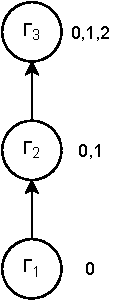
\includegraphics[scale = 1.1]{img/k4.pdf}
  \end{figure}
  Avendo quindi che:
  \begin{itemize}
    \item $P(\Gamma_0)=\{0\}$
    \item $P(\Gamma_1)=\{0,1\}$
    \item $P(\Gamma_2)=\{0,1,2\}$
  \end{itemize}
  Avendo rispettata la monotonia.\\
  Se avessi avuto, ad esempio, con rispettivo modello di Kripke:
  \begin{itemize}
    \item $P(\Gamma_0)=\{0\}$
    \item $P(\Gamma_1)=\{1\}$
    \item $P(\Gamma_2)=\{3,1\}$
  \end{itemize}
  Non avrei avuto una situazione valida.\\
  Ovviamente una situazione del tipo:
  \begin{itemize}
    \item $P(\Gamma_0)=\{0\}$
    \item $P(\Gamma_1)=\{0,1\}$
    \item $P(\Gamma_2)=\{0,1,3\}$
  \end{itemize}
  è valida, non avendo indicazioni sulla natura dei parametri ma solo sul fatto
  che devono aumentare in numero. Quindi è valida anche una situazione del tipo:
  \begin{itemize}
    \item $P(\Gamma_0)=\{0\}$
    \item $P(\Gamma_1)=\{0,1\}$
    \item $P(\Gamma_2)=\{0,1,3,5,9\}$
  \end{itemize}
  Ovviamente gli elementi dei nodi precedenti devono essere presenti anche nei
  nodi successivi, insieme però ad un numero arbitrario di nuovi elementi.
\end{esempio}
Vediamo ora il significato di ``vero'' per le formule predicative della logica
intuizionistica in un modello di Kripke, come appena specificato. Vediamo quini
i due casi, quello per $\exists$ e quello per $\forall$. \\
\textbf{Non si considerano formule aperte, $A$ è sempre chiusa}.
\begin{definizione}
  Si dice che, dato un nodo $\Gamma$ di un modello di Kripke $K$ per la logica
  predicativa intuizionistica, si ha che, per l'operatore esistenziale:
  \[\Gamma\vDash \exists xA(x)\iff \exists\, a\in P(\Gamma)\mbox{
      t.c. }\Gamma\vDash A(a)\]
  Quindi nel nodo $\Gamma$ è vera la formula $\exists xA(x)$ sse esiste un certo
  parametro $a$ nell'insieme dei parametri di $\Gamma$ tale per cui $A(a)$ è
  vero in $\Gamma$. Non ci interessiamo di tutti i vari $\Gamma'$ in relazione
  $R$ con $\Gamma$ quindi la definizione di ``essere vero'' per un esistenziale
  intuizionista coincide con la definizione classica della verità di un
  esistenziale, considerando un unico nodo del modello.\\
  Questa definizione sembra in contraddizione con la definizione della
  \textbf{proprietà dell'esplicita definibilità} della 
  logica intuizionistica, che dice che se si dimostra intuizionisticamente la
  formula $\exists x A(x)$ allora deve esistere un termine chiuso $t$ per cui si
  riesca a dimostrare $A(t)$ in logica intuizionistica. Questo però vedremo non
  accade, non avendo questa contraddizione.
\end{definizione}
\begin{definizione}
  Si dice che, dato un nodo $\Gamma$ di un modello di Kripke $K$ per la logica
  predicativa intuizionistica, si ha che, per l'operatore universale:
  \[\Gamma\vDash \forall xA(x)\iff \forall \,\Gamma' \mbox{ t.c. }\Gamma'
    R\,\Gamma \mbox{ e } \forall a \mbox{ t.c }a\in P(\Gamma')\mbox{ si ha }
    \Gamma'\vDash A(a)\]
  Quindi, per vedere che la formula $\forall xA(x)$ sia vera in un nodo
  $\Gamma$, bisogna vedere tutti i nodi di $K$ in relazione $R$ con $\Gamma$ e
  bisogna vedere tutti i parametri di questi nodi, verificando che in tutti
  questi nodi, per tutti i parametri, sia vera $A(a)$.\\
  Si ha in questo caso un'enorme differenza con la logica classica, dove non si
  ha questa ``stratificazione'' degli stati di conoscenza, avendo qui che
  $A(a)$ deve essere vero per tutti i parametri e in tutti i nodi accessibili
  da $\Gamma$.\\
  Dimostrare un $\forall$ è quindi molto oneroso dovendo praticamente dire che è
  la formula è valida in tutti i modelli di Kripke.
\end{definizione}
Grazie a queste due definizioni sappiamo valutare in $\Gamma$ la formula ben
formata predicativa $A$, ovvero:
\[\Gamma\vDash A\]
Sapendo come valutare la formula, fissato un $\Gamma$ che appartiene ad un
modello predicativo di Kripke della logica intuizionistica.\\
\textbf{Se ha fosse stata aperta si dovrebbe studiare anche l'assegnamento alle
  variabili libere e includere tale assegnamento nella definizione di
  verità. Questo non viene approfondito nel corso}.\\
Vediamo quindi qualche esempio.
\begin{esempio}
  Prendiamo la formula:
  \[\neg\neg\forall x(A(x)\lor \neg A(x))\]
  Se fosse dimostrabile in logica intuizionistica significa che è valida, non
  esistendo contromodelli. In caso non fosse dimostrabile si avrebbe almeno un
  modello di Kripke che non la rende vera.\\
  Una formula di questo tipo, a livello proposizionale senza $\forall$ ed
  $\exists$, terrebbe in considerazione il teorema
  di Kolmogorov-Glivenko, dicendo che se una formula è valida classicamente la
  sua doppia negazione lo è intuizionisticamente. Ma purtroppo questo teorema
  non si trasferisce automaticamente in logica predicativa, anche se il terzo
  escluso predicativo, presente nella nostra formula, $\forall x(A(x)\lor \neg
  A(x))$ è valido il logica classica. \\
  Vediamo che la formula non è dimostrabile intuizionisticamente, esistendo un
  nodo $\Gamma$ che non rende vera la doppia negazione del terzo escluso
  predicativo. \\
  Costruiamo il seguente modello infinito (\textit{il prof usa archi non
    orientati ma metto entrambe le versioni}):
   \begin{figure}[H]
    \centering
    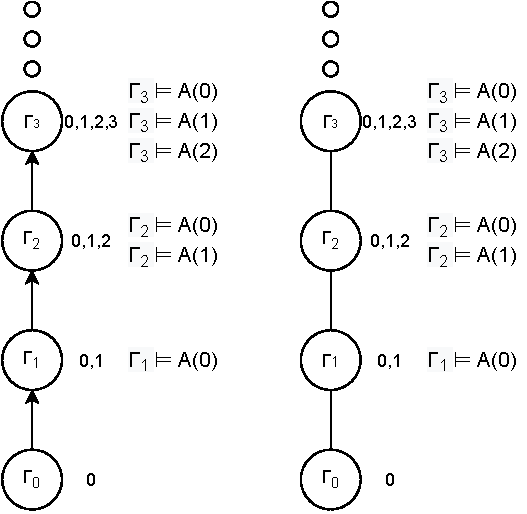
\includegraphics[scale = 0.9]{img/k5.pdf}
  \end{figure}
  Si hanno quindi i nodi, infiniti con ogni nodo associato ad un numero naturale
  sempre crescente, così specificati:
  \begin{itemize}
    \item $\Gamma_0$ contiene il parametro $\{0\}$ e non rende vera nessuna
    formula 
    \item $\Gamma_1$ contiene i parametri $\{0,1\}$ e rende vera $A(0)$
    \item $\Gamma_2$ contiene i parametri $\{0,1,2\}$ e rende vera $A(0)$ e
    $A(1)$ 
    \item $\Gamma_3$ contiene i parametri $\{0,1,2,3\}$ e rende vera $A(0)$,
    $A(1)$ e $A(2)$
    \item etc$\ldots$
  \end{itemize}
  Vediamo in primis se la funzione $P$ è strettamente monotona crescente. Si ha
  che: 
  \begin{itemize}
    \item $P(\Gamma_0)=\{0\}$
    \item $P(\Gamma_1)=\{0,1\}$
    \item $P(\Gamma_2)=\{0,1,2\}$
    \item $P(\Gamma_3)=\{0,1,2,3\}$
    \item etc$\ldots$
  \end{itemize}
  e quindi la funzione che associa i parametri ai nodi è strettamente monotona
  crescente.\\ 
  Vediamo ora la funzione di forcing, che deve rispettare il fatto che se una
  formula è vera in un $\Gamma$ allora è vera anche i $\Gamma_i$ successivi. Si
  ha che:
  \begin{itemize}
    \item in $\Gamma_0$ non è vero nulla
    \item in $\Gamma_1$ è vera $A(0)$ ma è falsa $A(1)$
    \item in $\Gamma_2$ sono vere $A(0)$ e $A(1)$ ma è falsa $A(2)$
    \item in $\Gamma_3$ sono vere $A(0)$, $A(1)$ e $A(2)$ ma è falsa $A(3)$
    \item etc$\ldots$
  \end{itemize}
  Quindi viene rispettato il fatto che se la formula è vera in un nodo viene
  rimane vera anche in tutti quelli successivi.\\
  Possiamo quindi dire, per le due considerazioni appena fatte, che questo è
  effettivamente un modello di Kripke per la logica predicativa
  intuizionistica. \\
  Vediamo ora questo è un contromodello (e lo possiamo fare solo dopo aver
  dimostrato che è effettivamente un modello di Kripke valido per la logica
  predicativa intuizionista) per la formula in analisi, dicendo che 
  $\Gamma_0$ non rende vera la formula in questione che quindi non può essere
  valida e dimostrabile.\\
  La doppia negazione significa trovare almeno uno stato in cui è vera la
  formula quindi devo trovare, da $\Gamma_0$, uno stato in cui è vera
  $\forall x(A(x)\lor \neg A(x))$. \\
  Per avere che la formula sia valida in $\Gamma_0$ dovrei avere che in tutti i
  nodi successivi deve essere vero $A(\cdot)$ per i parametri di quei nodi o
  $\neg A(\cdot)$ per i parametri di quei nodi. \\
  In $\Gamma_0$ $A(0)$ non è vera. Per essere vero $\neg A(0)$ dovrei
  avere che in tutti i nodi successivi deve essere falso $A(0)$ ma già in
  $\Gamma_1$ è vera. Quindi $\Gamma_0$ non può essere il nodo che stiamo
  cercando. Per lo stesso ragionamento nessuno dei nodi può esserlo, avendo che
  in uno stato la formula è vera 
  per i parametri del nodo precedente e non per il nuovo parametro
  introdotto, sempre tenendo conto che il modello è infinito. Questo accadrebbe
  anche aggiungendo nuovi stati sempre con la 
  logica per la quale in un certo stato la formula è vera 
  per i parametri del nodo precedente e non per il nuovo parametro
  introdotto.\\
  Si è giunti quindi a dire che in $\Gamma_0$ la formula $\forall x(A(x)\lor
  \neg A(x))$ non vale. Dato che basta un solo contromodello posso dire che la
  formula non è valida per la logica predicativa intuizionistica.\\
  Se il modello fosse finito il ragionamento fatto non funzionerebbe nell'ultimo
  nodo, con la formula che sarebbe verificata nell'ultimo nodo (basti pensare al
  fatto che se ci fermassimo in $\Gamma_3$ avrei la formula verificata). \\
  \textbf{Quindi il teorema di Kolmogorov-Glivenko, così come lo abbiamo dato,
    non è estendibile dal proposizionale al predicativo}.\\
  \textit{Spiegazione più dettagliata a pagina 49 del Fitting}.
\end{esempio}
Abbiamo visto come non si possa usare il teorema di Kolmogorov-Glivenko ma
esiste un metodo per tradurre formule valide classicamente in formule valide
intuizionisticamente.
\begin{definizione}
  Definiamo il \textbf{metodo di traduzione} $\tau$ come il metodo che dice:
  \begin{itemize}
    \item $\tau(A)=\neg\neg A$, con $A$ atomica
    \item $\tau(A\land B)=\tau(A)\land \tau (B)$
    \item $\tau(A\to B)=\tau(A)\to \tau (B)$
    \item $\tau(\forall x A(x))=\forall x\tau(A(x))$
    \item $\tau(A\lor B)=\neg(\neg \tau(A)\land \neg\tau(B))$
    \item $\tau(\exists x A(x))=\neg\forall x\neg\tau(A(x))$
  \end{itemize}
  Si noti come le due traduzioni ``strane'' sono le ultime due, su $\lor$ e
  $\exists$, dovendo rispettare per la prima la \textbf{proprietà di
    disgiunzione} e per la seconda la \textbf{proprietà dell'esplicita
    definibilità}. \\
  Il $\neg$ resta primitivo e non si traduce. Quindi si ha:
  \[\tau(\neg A)=\neg\tau(A)\]
\end{definizione}
\begin{teorema}
  Si ha quindi il \textbf{teorema della traduzione negativa della logica
    predicativa classica nella logica predicativa intuizionistica} e
  si dimostra che:
  \[\vdash_{CL}A\iff \vdash_{INT}\tau(A)\]
  Questo teorema, nonché il calcolo sopra definito di $\tau$, è stato ideato da
  G\"{o}del. 
\end{teorema}
\textit{Questo teorema è l'equivalente predicativo del teorema di
  Kolmogorov-Glivenko del caso proposizionale.}
\begin{esempio}
  Vediamo la traduzione di $\forall x(A(x)\lor\neg A(x))$ dal classico
  all'intuizionistico per vedere che non porta, come dimostrato nell'esempio
  precedente, alla doppia negazione della stessa.\\
  Vediamo quindi:
  \[\tau(\forall x(A(x)\lor\neg A(x)))\]
  che è, per la traduzione del $\forall$:
  \[\forall x\tau(A(x)\lor \neg A(x))\]
  che diventa, per la traduzione di $\lor$:
  \[\forall x\neg(\neg \tau(A(x))\land \neg \tau(\neg A(x)))\]
  che diventa, per la traduzione delle formule atomiche (ricordando che non si
  ha la traduzione di $\neg$ che resta primitiva): 
  \[\forall x\neg(\neg\neg \neg A(x)\land\neg\neg\neg\neg A(x))\]
  che è dimostrabile intuizionisticamente per il teorema appena descritto,
  avendo applicato le regole di traduzione. Tale formula è dimostrabile in
  deduzione naturale e tramite, vedremo più avanti, il calcolo a tableau. Per
  tale formula, ovviamente, non si trovano contromodelli di Kripke.\\
  Si noti come sia ben diversa dalla semplice doppia negazione della formula,
  come accadeva nel caso proposizionale.
\end{esempio}
\newpage
\subsection{Tableaux}
Passiamo quindi allo studio dei tableaux nel caso della logica intuizionistica
predicativa. \\
Si studiano quindi le T regole e le F regole dei due quantificatori, dato $S$
insieme di formule ben formate, secondo Fitting:
\begin{table}[H]
  \centering
  \Large
  \begin{tabular}{c||c|c}
    quantificatore & T-regola & F-regola\\
    \hline
    $\exists$ & $\frac{S,T\,\exists x A(x)}{S,TA(a)}${\small{(con a nuovo)}}
                             & $\frac{S,F\,\exists x A(x)}{S,FA(a)}$\\
    $\forall$ & $\frac{S,T\,\forall x A(x)}{S,TA(a)}$
                              & $\frac{S,F\,\forall x A(x)}{S_T,
                                FA(a)}${\small{(con a nuovo)}}\\
    \hline
  \end{tabular}
\end{table}
Quindi nel $T\,\exists$ si ha che $a$ non deve essere mai apparsa prima nel
tableau. Le due T-regole sono le medesime della logica classica, anche se la
semantica dei due quantificatori ben diversa.\\
\textbf{Questo è un calcolo corretto e completo per la logica predicativa
  intuizionistica, tramite tableaux, secondo Fitting.}\\
Ovviamente tutte le formule dimostrabili il deduzione naturale, anche in questo
caso, devono essere dimostrabili coi tableaux, e viceversa le formule non
dimostrabili in deduzione naturale non devono esserlo coi tableaux.\\
In intuizionismo tutte le definizioni di dimostrazione a tableaux chiuso e
branching fatte nel caso proposizionale si traspongono nel predicativo. Quindi
anche in questo caso si parte con la formula segnata $F$ e si deve arrivare ad
un tableau chiuso per dimostrarlo. Se nessun tableaux è chiuso, anche in questo
caso, la formula non è dimostrabile.\\
La logica predicativa intuizionistica, così come quella classica, è
semi-decidibile e quindi non si ha un algoritmo di dimostrazione come per la
logica proposizionale classica o intuizionistica, dove un tableau finisce
sempre. A livello predicativo questo non succede avendo solo un metodo di
semi-decisione che ci dice che se una formula è valida posso dimostrarla ma se
non è valida il meccanismo per stabilire che non è dimostrabile può non
terminare mai. Nel 1936 Churh ha dimostrato che basta avere un simbolo di
funzione binaria e un simbolo di predicato binario per costruire una formula
indecidibile. Questa è una conseguenza del teorema di incompletezza di
G\"{o}del per l'aritmetica di Peano.
\newpage
Vediamo quindi qualche esempio.
\begin{esempio}
  Iniziamo con il terzo escluso predicativo:
  \[\nvdash_{INT}\forall x(A(x)\lor \neg A(x))\]
  Si ha quindi:
  \begin{gather*}
    \frac{F\forall x(A(x)\lor \neg A(x))}{}F\forall\\
    \frac{F (A(a)\lor \neg A(a))}{}F\lor\\
    \frac{FA(a),F\neg A(a)}{}F\neg\\
    TA(a)
  \end{gather*}
  Avendo che il tableau non chiude e non avendo possibilità di backtracking.\\
  In logica classica $F\neg$ non avrebbe ristretto a $S_T$ e quindi il tableau
  sarebbe stato chiuso.
\end{esempio}
\begin{esempio}
  Vediamo la doppia negazione del terzo escluso predicativo:
  \[\nvdash_{INT}\neg\neg\forall x(A(x)\lor \neg A(x))\]
  \begin{gather*}
    \frac{F\neg\neg\forall x(A(x)\lor \neg A(x))}{}F\neg\\
    \frac{T\neg\forall x(A(x)\lor\neg A(x))}{}T\neg\\
    \frac{F\forall x(A(x)\lor \neg A(x))}{}F\forall\\
    \frac{F (A(a)\lor \neg A(a))}{}F\lor\\
    \frac{FA(a),F\neg A(a)}{}F\neg\\
    TA(a)  
  \end{gather*}
  Avendo che il tableau non chiude e non avendo possibilità di backtracking.\\
  In logica classica $F\neg$ non avrebbe ristretto a $S_T$ e quindi il tableau
  sarebbe stato chiuso.\\
  Però ricordiamo che con il $T\neg$ di Fitting potrebbe essere necessario
  ripetere la formula.
  Chiamo quindi:
  \[\alpha=T\neg\forall x(A(x)\lor\neg A(x))\]
  e quindi si ha:
  \begin{gather*}
    \frac{F\neg\neg\forall x(A(x)\lor \neg A(x))}{}F\neg\\
    \frac{T\neg\forall x(A(x)\lor\neg A(x))}{}T\neg\\
    \frac{\alpha,F\forall x(A(x)\lor \neg A(x))}{}
  \end{gather*}
  A questo punto potrei sviluppare $\alpha$ ma come visto sarebbe
  inutile. Sviluppo quindi $F\forall$:
  \begin{gather*}
    \frac{\alpha,F\forall x(A(x)\lor \neg A(x))}{}F\forall\\
    \frac{\alpha, F(A(a)\lor \neg A(a))}{}F\lor\\
    \frac{\alpha, FA(a), F\neg A(a)}{}
  \end{gather*}
  Potrei fare $\alpha$ (che è un $T$) ma avrei poi una restrizione che
  taglierebbe le due $F$. L'unica strategia rimanente è fare $F\neg$:
  \begin{gather*}
    \frac{\alpha, FA(a), F\neg A(a)}{}F\neg\\
    \frac{\alpha, TA(a)}{}\\
    \frac{F\forall x(A(x\lor\neg A(x))), TA(a)}{}F\forall\\
    \frac{F(A(b)\lor\neg A(b)), TA(a)}{}F\lor\\
    FA(b), F\neg A(b), TA(a)
  \end{gather*}
  Dove nel penultimo passaggio non posso usare la stessa $a$ di $TA(a)$. Si ha
  quindi che comunque il tableau non chiude, avendo $TA(a)$ e $FA(b)$.
\end{esempio}
Entrambi questi esempi sono coerenti con quanto visto con la deduzione
naturale.\\
Vediamo anche una formula dimostrabile, anche perché è più semplice usare i
tableaux che la deduzione naturale, quindi in caso prima verifico coi tableaux e
poi con la deduzione naturale.
\begin{esempio}
  Vediamo:
  \[\vdash_{INT} \neg\exists x A(x)\iff \forall x\neg A(x)\]
  Partiamo con:
  \[\vdash_{INT} \neg\exists x A(x)\to \forall x\neg A(x)\]
  Avendo:
  \begin{gather*}
    \frac{F(\neg\exists x A(x)\to \forall x\neg A(x))}{}F\to\\
    \frac{T\neg\exists xA(x), F\forall x\neg A(x)}{}
  \end{gather*}
  Ma qui ci serve una strategia che rispetti il fatto che nelle regole
  predicative non devo avere $a$ giù usate.\\
  Proseguo con $F\forall$ per le regole di restrizione e che impone il parametro
  nuovo. Segnalo comunque il backtracking *:
  \begin{gather*}
    \frac{*T\neg\exists xA(x), F\forall x\neg A(x)}{}F\forall\\
    \frac{T\neg \exists x A(x), F\neg A(a)}{}
  \end{gather*}
  Scelgo quindi di fare il $F\neg$, segnalando il backtracking **, perché genera
  qualcosa che non verrà mai cancellato nel tableau:
  \begin{gather*}
    \frac{**T\neg \exists x A(x), F\neg A(a)}{}F\neg\\
    \frac{T\neg \exists x A(x), T A(a)}{}T\neg\\
    \frac{F\exists xA(x), TA(a)}{}F\exists\\
    FA(a), TA(a)
  \end{gather*}
  Avendo che il tableau chiude, senza bisogno di backtracking (si noti per di
  più che quella fatta è la scelta migliore, forse l'unica che fa chiudere il
  tableau).\\ 
  Verifico ora la conversa:
  \[\vdash_{INT} \forall x\neg A(x)\to \neg\exists x A(x) \]
  Si ha quindi:
  \begin{gather*}
    \frac{F(\forall x\neg A(x)\to \neg\exists x A(x))}{}F\to\\
    \frac{T\forall x\neg A(x), F\neg\exists x A(x)}{}
  \end{gather*}
  Scelgo quindi di fare il $F\neg$, segnalando il backtracking *, perché avere
  poi $T\exists$ che introduce $a$ mentre il $T\forall$ non lo richiede nuovo:
  \begin{gather*}
    \frac{*T\forall x\neg A(x), F\neg\exists x A(x)}{}F\neg\\
    \frac{T\forall x\neg A(x), T\exists xA(x)}{}
  \end{gather*}
  Scelgo ora di fare $T\exists$ per ottenere il nuovo $a$:
  \begin{gather*}
    \frac{**T\forall x\neg A(x), T\exists xA(x)}{}T\exists\\
    \frac{T\forall x\neg A(x), TA(a)}{}T\forall\\
    \frac{T\neg A(a), TA(a)}{}T\neg\\
    FA(a), TA(A)
  \end{gather*}
  Avendo che il tableau chiude, senza bisogno di backtracking.
\end{esempio}
Questo è quindi il calcolo ``puro'' di Fitting. Vedremo poi le ottimizzazioni
come nel caso dei tableaux proposizionali, fatte da Moscato e dai suoi colleghi
(mentre Dyckhoff sul predicativo intuizionista ci mise 10 anni per i sequenti).
\subsection{Tableaux Estesi}
Il prossimo passo è quindi quello di aggiungere il terzo segno anche al caso
predicativo, ottimizzando poi il $T\to$, dovendo comprendere, tra gli
antecedenti dell'implicazione, un possibile $\forall$ o un possibile $\exists$
(ricordando che il $T\to$ si divide in vari casi a seconda dell'antecedente).\\
\textit{Su Moodle c'è anche un paper sulla differenza di $F\exists$ nel calcolo
  classico e nel calcolo intuizionista, che non richiede duplicazione nel caso
  intuizionista a differenza di quello classico.}\\
Vediamo quindi l'estensione del calcolo con le eventuali ripetizioni, estensione
che è abbastanza ``naturale'': 
\begin{table}[H]
  \centering
  \Large
  \begin{tabular}{c||c|c}
    quantificatore & T-regola & F-regola\\
    \hline
    $\exists$ & $\frac{S,T\,\exists x A(x)}{S,TA(a)}${\small{(con a nuovo)}}
                             & $\frac{S,F\,\exists x A(x)}{S,FA(a)}$\\
    $\forall$ & $\frac{S,T\,\forall x A(x)}{S,TA(a),T\,\forall x A(x)}$
                              & $\frac{S,F\,\forall x A(x)}{S_C,
                                FA(a)}${\small{(con a nuovo)}}\\
    \hline
  \end{tabular}
\end{table}
Il $T\forall$ e il $T\exists$ valgono anche a livello di logica classica. Nella
$F\forall$ si restringe $S$ a $S_C$, ovvero a contenere solo $T$ formule e $F_C$
formule, variando solo la restrizione rispetto a Fitting, dove si aveva $S$
ristretto a $S_T$. In merito a $F\exists$ nel caso classico si avrebbe la
ripetizione di $F\,\exists x A(x)$ mentre nel caso intuizionistico no, imponendo
che $a$ sia un $a$ qualsiasi ma ``una volta sola'', non avendo la ripetizione.\\
Nel caso di Fitting le differenze con il caso classico non erano esplicitate non
essendo esplicitate le ripetizioni.\\
A livello classico $F\,\exists x A(x)$ è realizzata quando $A(a)$ è $\bot$ per
ogni $a$, per questo in logica classica si ripete. In logica intuizionistica non
ripeto, per un vincolo semantico dell'esistenziale a livello intuizionistico,
essendo l'esistenziale locale dal punto di vista semantico ad un unico nodo del
modello di Kripke si che fissata $a$ non posso riusare $F\,\exists x A(x)$.\\
Solo l'$F\forall$ restringe a $S_C$.\\
Manca però l'uso del segno $F_C$ per completare il calcolo:
\begin{table}[H]
  \centering
  \Large
  \begin{tabular}{c||c}
    quantificatore & $\mbox{F}_C$-regola\\
    \hline
    $\exists$ & $\frac{S,F_C\,\exists x A(x)}{S,F_CA(a),F_C\,\exists x A(x)}$\\
    \hline
    $\forall$ & $\frac{S,F_C\,\forall x A(x)}{S_C,FA(a), F_C\,\forall xA(x)}
                \mbox{(con a nuovo)}$
  \end{tabular}
\end{table}
Si noti come nell'$F_C\forall$ si passi da una formula $F_C$ ad una formula $F$
che potrebbe essere tagliata da altre regole e quindi, per garantire il 
segno certo $F_C$, bisogna ripetere la formula $F_C\,\forall x A(x)$. Scrivere
$F_CA(a)$ non sarebbe corretto secondo la semantica della logica
intuizionistica. Non si ha lo stesso vantaggio del caso proposizione usando
$F_C$, indebolendo al formula destrutturata, avendo $FA(a)$ che non si può
rafforzare con $F_C$ venendo a mancare le dimostrazioni di correttezza del
calcolo in caso, e ripetendo la formula strutturata.\\
Invece in $F_C\exists$ ripeto la formula posso anche mettere $F_CA(a)$,
potendolo ripetere per ogni costante, $F_CA(b)$, $F_CA(c)$ etc$\ldots$ Non viene
quindi indebolita la formula e si possono creare tutte le varianti per le
costanti che servono. Si nota la differenza di realizzabilità di $F_C\exists$
rispetto a $F\exists$ in quanto il segno $F_C$ è il $\neg$ e quindi è un
$T\neg$, che va a prendere tutti i livelli del modello di Kripke, dicendo, con
$T\neg A$ che de $A$ deve essere falso in tutti i nodi, avendo quindi $F_C$,
contrapposto a $F$ che significa falso in un solo nodo.\\
Restano da analizzare le due regole del $T\to$ con antecedente un esistenziale e
un universale.
\begin{table}[H]
  \centering
  \Large
  \begin{tabular}{c||c}
    quantificatore & $T\to$regola\\
    \hline
    $\exists$ & $\frac{S,T\,\exists x A(x)\to B}{S,T(\forall x(A(x)\to B))}$\\
    \hline
    $\forall$ & $\frac{S,T\,\forall x A(x)\to B}{S,F\,\forall xA(x),T\,\forall
                xA(x)\to B/ S, TB}$
  \end{tabular}
\end{table}
Si noti come nel caso universale bisogna dividere il tableau di due, avendo un
$T\to$ e nel primo caso, avendo $F$ dell'antecedente devo anche ripetere
l'intera formula. In questo caso non si hanno grandi vantaggi a differenza del
proposizionale. Non si può fare nulla di più sul caso universale.\\
Il caso esistenziale porta invece un vantaggio in quanto avendo un'implicazione
con un esistenziale la si trasforma in un'implicazione di un quantificatore
universale su tutta la formula, diminuendo la complessità dell'antecedente,
avvicinandoci al caso delle formule atomiche. L'implicazione ora in se non ha
più un quantificatore per l'antecedente, in quanto ora riguarda solo l'intera
formula. Si è ottenuto un vantaggio computazionale.\\
Ho quindi un \textbf{calcolo corretto e completo per la logica intuizionistica
  predicativa} ma bisogna dimostrarlo. \\
Vediamo quindi in primis che sia \textbf{corretto}. Prendo quindi una formula
predicativa non dimostrabile intuizionisticamente e vedo che lo sia anche con il
calcolo a tableaux esteso, non avendo alcun tableaux che chiuda. Si ha un
risultato teorico, il \textbf{lemma di Lindembuam} (\textit{potrebbe essere
  errato il nome del lemma}), che dice che non si ottiene mai il tableau
chiuso, anche senza dover ``provare'' con tutte le costanti (che sarebbe un
conto infinito e inutile).
\begin{esempio}
  Usiamo quindi, ad esempio, la formula della doppia negazione del principio del
  terzo escluso predicativo:
  \[\nvdash_{INT} \neg\neg \forall x(A(x)\lor \neg A(x))\]
  di cui sa già esistere il contromodello.\\
  Vediamo quindi il calcolo:
  \begin{gather*}
    \frac{F \neg\neg \forall x(A(x)\lor \neg A(x))}{}F\neg\\
    \frac{T\neg \forall x (A(x)\lor \neg A(x))}{}T\neg\\
    \frac{F_C\forall x (A(x)\lor \neg A(x))}{}F_C\forall\\
    \frac{*F(A(a)\lor\neg A(a)),F_C\forall x (A(x)\lor \neg A(x))}{}
  \end{gather*}
  Se applicassi $F_C\forall$ tornerei alla stessa formula (si elimina l'$F$ ma
  si reintroduce la stessa formula) quindi applico $F\lor$ e posso anche
  togliere la notazione del backtracking in quanto sarei in un loop che non
  porterebbe ad altri risultati fino che non si sceglie di fare $F\lor$:
  \begin{gather*}
    \frac{F(A(a)\lor\neg A(a)),F_C\forall x (A(x)\lor \neg A(x))}{}F\lor\\
    \frac{FA(a), F_C\forall x(A(x)\lor\neg A(x)),F\neg A(a)}{} 
  \end{gather*}
  Se faccio $F\neg$ elimino $FA(a)$ mentre se faccio $F_C\forall$ elimino sia
  $FA(a)$ che $F\neg A(a)$. Avrei infatti:
  \begin{gather*}
    \frac{FA(a), F_C\forall x(A(x)\lor\neg A(x)),F\neg A(a)}{} F\neg\\
    \frac{F_C\forall x(A(x)\lor\neg A(x)), TA(a)}{}F_C\forall\\
    FA(b)\lor\neg A(b),F_C\forall x(A(x)\lor\neg A(x)),TA(a)
  \end{gather*}
  con la risoluzione dell'or che porterebbe comunque a non poter chiudere avendo
  $a$ e $b$. Inutile dire cosa succede se faccio subito $F_C\forall$ visto che
  si cancella tutto e avendo che sicuro non chiuderà mai il tableau.\\
  Non avendo tableaux che chiudono si conferma la non dimostrabilità della
  formula in logica intuizionistica predicativa.
\end{esempio}
Si potrebbe vedere che in tutti i casi le formule intuizionistiche predicative
non dimostrabili lo restano anche con questo nuovo calcolo esteso.
\begin{esempio}
  Vediamo anche un esempio di formula dimostrabile:
  \[\vdash_{INT}\exists x \neg A(x)\to \neg\forall xA(x)\]
  Si ha:
  \begin{gather*}
    \frac{F\exists x \neg A(x)\to \neg\forall xA(x)}{}F\to\\
    \frac{*T\exists x\neg A(x),F\neg\forall x A(x)}{}
  \end{gather*}
  Scelgo di fare $F\neg$ che tanto non taglia la $T$.
  \begin{gather*}
    \frac{*T\exists x\neg A(x),F\neg\forall x A(x)}{}F\neg\\
    \frac{**T\exists x\neg A(x), T\forall x A(x)}{}
  \end{gather*}
  Scelgo di applicare il $T\exists$.
  \begin{gather*}
    \frac{**T\exists x\neg A(x), T\forall x A(x)}{}T\exists\\
    \frac{***T\neg A(a),T\forall xA(x)}{}
  \end{gather*}
  Scelgo di applicare il $T\neg$:
  \begin{gather*}
    \frac{***T\neg A(a),T\forall xA(x)}{}T\neg\\
    \frac{F_C A(a),T\forall xA(x)}{}T\forall\\
    \frac{F_C A(a), TA(a)}{}
  \end{gather*}
  Avendo che il tableau chiude.\\
  Si può vedere che altre scelte avrebbero portato il tableau a non chiudere
  mentre ci sono altri percorsi che avrebbero comunque chiuso (ad esempio
  facendo l'altra scelta in **).
\end{esempio}
\subsection{Teoremi di Completezza e Validità}
\textbf{Argomento accennato a lezione, ``bigino'' su Moodle}.\\
Parliamo quindi dei \textbf{teoremi di completezza e validità della logica
  predicativa intuizionistica}, nella versione del calcolo, quella senza
duplicazioni proposizionali. Le dimostrazioni dei due teoremi sono lunghe e
complesse e quindi vengono solo accennate.
\begin{definizione}
  Un insieme $S$ di formule segnate è detto \textbf{insieme consistente} se non
  vi è alcun tableau che chiude per $S$, qualsiasi siano i backtracking fatti.\\
  Se $S$ quindi contiene una formula non dimostrabile $A$ si dice che $S$ è
  consistente, in quanto nessun tableau chiuderà mai.
\end{definizione}
\begin{definizione}
   Dato un insieme $S$ di formule segnate si definisce un insieme, detto
   \textbf{insieme di riferimento} $\pi$, come l’insieme dei parametri che
   compaiono in $S$.
\end{definizione}
\begin{teorema}[Teorema di Validità]
  Data una formula $A$, per cui esiste un tableau chiuso per $FA$, allora la
  formula $A$ è valida nella logica predicativa intuizionistica.\\
  In altri termini le regole del calcolo a tableaux preservano la verità e che
  se una formula, segnata $F$, ha un tableau chiuso allora alla fine avrò
  configurazioni che contengono $TA$ e $FA$. Essendo perciò partiti con $FA$ si
  arriva ad una contraddizione e quindi vale che la formula è vera (è quello che
  abbiamo sempre fatto e questo è il teorema dietro a questo).
\end{teorema}
\begin{proof}
  Si ricorda che una formula segnata $T$ è realizzabile quando esiste un nodo
  del modello di Kripke in cui la formula è vera. Una formula segnata $F$ è
  realizzabile quando nel nodo in analisi la formula non è vera e la
  formula segnata $F_C$ è realizzabile quando per ogni nodo accessibile da
  quello di partenza non è vera la formula.\\
  Osservando che se una configurazione è realizzabile prima
  dell’applicazione di una regola del calcolo, lo sarà anche la configurazione
  ottenuta dopo l’applicazione della regola stessa, e quindi in un nodo del
  modello di Kripke che realizzava la configurazione di partenza. \\
  Supponiamo di avere un tableau chiuso per $FA$. Si ha quindi che $FA$ non è
  realizzabile e quindi $A$ è forzata in tutti i modelli di Kripke. 
\end{proof}
\begin{lemma}
  Se un insieme $I$ di formule segnate è consistente si ha che esiste un modello
  di Kripke $K_I$ e si ha che esiste un nodo $g$ di $K_I$ che realizza $I$. \\
  In altri termini insiemi di formule segnate consistenti hanno sempre un
  modello di Kripke che le realizza.\\ 
  Questo lemma è legato al fatto che si parla di semantic tableaux.\\
  La dimostrazione di tale lemma si fa in modo molto complesso.
\end{lemma}
\begin{lemma}
  Per ogni insieme $I$ consistente di formule segnate, per ogni modello di
  Kripke $K_I$, per ogni nodo $S$ di $K_I$, per ogni formula $H$ di ogni
  saturato $S^*$ di $S$ si ha che $H$ è realizzata in $S$. \\
  La dimostrazione di tale lemma si fa in modo molto complesso, per induzione.
\end{lemma}
\begin{definizione}
  Si definiscono i \textbf{saturati} come insiemi di formule, in questo caso
  segnate, che si ottengono applicando alle formule stesse le regole di
  inferenza. 
\end{definizione}
\begin{teorema}[Teorema di Completezza]
  Se una data formula $A$ è valida nella logica predicativa intuizionistica
  allora esiste un tableau chiuso per $FA$.\\
  In altri termini si può trovare un tableau che chiude per $FA$ e quindi $FA$
  non sarà mai realizzabile.
\end{teorema}
\begin{proof}
  Dato un insieme di formule segnate $S$ consistente, che contiene una formula
  $H$, definiamo un insieme $R$ come una estensione consistente di $H$ in
  $S$. Si ha che $R$ è un insieme contiene una delle formule ottenute applicando
  la regola dei tableau ad $H$ per cui: 
  \[(S - \{H\})\cup R\]
  sia consistente. Tale riduzione quindi deve essere consistente. Dove non c'è
  branching è fuori discussione che la riduzione porti ad una configurazione
  consistente, ovvero ad un $S'$ consistete. Quando $H$ è invece una formula per
  la quale la regola in suo comporta branching si che bisogna scegliere il
  percorso che mantiene la consistenza nella nuova configurazione di formule.
  Lo stesso vale per tutte le formule che contengono variabili o riduzioni di
  variabili.\\
  Si hanno quindi due passi:
  \begin{itemize}
    \item \textbf{passo A}: \textit{costruzione dei saturati e di un
      nodo del modello di Kripke}. \\
    Le regole che non restringono $S$ a $S_C$ sono quelle che creano il nodo del
    modello attraverso i saturati. Il comportamento del calcolo quindi
    corrisponde alla costruzione del modello che si cerca per un insieme
    consistente. Detto in termini più semplici le formule che non restringono
    restano nello stesso nodo e arrivando in quel nodo del modello le formule
    atomiche andranno a forzare tutte quelle segnate $T$.\\
    In questo passo si ha che $H_j$ è formato da, con $A,B\in FBF$:
    \begin{itemize}
      \item $TA\land B$
      \item $TA\lor B$
      \item $T\neg A$
      \item $(TA\lor B)\to C$
      \item $(TA\land B)\to C$
      \item $(T\exists xA(x))\to B$
      \item $(T\forall xA(x))\to B$
      \item $FA\land B$
      \item $FA\lor B$
      \item $F_CA\lor B$
    \end{itemize}
    Ovvero tutte regole che non restringono mai $S$ a $S_C$.\\
    Si ha che la riduzione di $H_j$ al passo $i$, indicata con:
    \[R(H_j,i)\]
    è un'estensione consistente di $H_j$ dove l'estensione consistente è la
    scelta delle formule che si ottengono applicando alla formula stessa la
    regola specifica e scegliendo poi la parte consistente in caso di
    branching.\\
    Vediamo i casi di branching.\\
    Se $H_j$ è $TA\to B$, con $A$ atomica o negata, e $TB$ è
    un'estensione consistente di $H_j$ allora si ha che:
    \[R(H_j,i)=\{TB\}\]
    Se $H_j$ è $T(A\to B)\to C$ e $TC$ è
    un'estensione consistente di $H_j$ allora si ha che:
    \[R(H_j,i)=\{TC\}\]
    Per il teorema di completezza e l'uso dei saturati si sceglie quindi la
    parte con $TB$ nel primo esempio e e $TC$ nel secondo. Il teorema di
    completezza comporta quindi una possibile strategia, che porta a formule di
    complessità minore etc$\ldots$ 
    \item \textbf{passo B}: \textit{costruzione nodi successori del modello di
      Kripke}.\\
    Le regole che restringono $S$ a $S_C$ (ma non solo come vedremo) sono quelle
    che creano i nodi successori. Detto in termini più semplici le formule che
    restringono $S$ a $S_C$ costruiscono nodi successori rispetto alla radice
    del modello e in quei nuovi nodi saranno realizzate le formule $T$ e
    $F_C$.\\
    Si costruisce l'insieme dei nodi successori semplici $S'$ avendo $A$ come:
    \begin{itemize}
      \item $F\neg B$
      \item $F_C\neg B$
      \item $FB\to C$
      \item $F_CB\to C$
      \item $F_CB\land C$
      \item $F\forall xB(x)$
      \item $F_C\forall xB(x)$
    \end{itemize}
    Questo gruppo di formule altro non è che il gruppo delle formule le cui
    regole restringono $S$ a $S_C$. $S'$ è ottenuto da $S$ sostituendo $A$ con
    una delle sue estensioni consistenti in $S$ e cancellando tutte le formule
    segnate $F$. \\
    Nel caso di $A=F\exists xB(x)$, dove $S$ non restringe a $S_C$, si ha che
    $S'$ è ottenuto da $S$ sostituendo $A$ con $FB(t)$, per ogni parametro
    $t$. Tale formula è quindi realizzata nei nodi successori. Si creano quindi
    tanti $S'$ quanti sono i parametri contenuti 
    nell'insieme dei parametri di $S$, insieme che può crescere durante il
    processo. Si ricordi che tale regola richiede ripetizione nel caso classico
    ma non nel caso intuizionistico. La formula quindi non viene ripetuta ma si
    ha una sorta di ripetizione per ogni parametro nella dimostrazione del
    teorema di completezza.\\
    \textit{Si hanno altre costruzioni necessarie per arrivare alla completezza
      che non vengono qui elencate} 
  \end{itemize}
  Si costruisce quindi il modello di Kripke corrispondente a un insieme di
  formule segnate consistente $I$: 
  \[K_I=\langle G_i,R,\vDash\rangle\]
  tale che:
  \begin{itemize}
    \item gli elementi di $G_I$ corrispondono ad opportuni insiemi $S$
    consistenti (essendo $I$ consistente non potrei fare altrimenti)
    ottenuti nel \textit{passo A} e nel \textit{passo B}  
    \item per ogni nodo di $K_I$, l’insieme dei parametri sarà determinato dal
    \textit{passo A} e dal \textit{passo B}   
    \item in ogni nodo di $K_I$ forziamo in esso tutte le formule atomiche
    segnate $T$ di $S$ 
  \end{itemize}
  Usando quindi i due lemmi visti sopra possiamo dimostrare effettivamente
  il teorema di completezza, ovvero che se una formula $A$ è valida
  intuizionisticamente, esiste un tableau chiuso per $FA$.\\
  \textit{I dettagli della dimostrazione vengono trascurati}.  \\
  Si supponga per assurdo che non esista tale tableau chiuso, avendo quindi che
  $\{FA\}$ è consistente. Si ha però che, allora per quanto visto, $\{FA\}$ è
  realizzabile (essendo consistete), ma questo è un assurdo perché la formula
  $A$ è valida e quindi non può esistere un modello che realizza $FA$,
  dimostrando così il teorema. 
\end{proof}

\chapter{Logica di Kuroda}
Kuroda è un ricercatore giapponese che si è chiesto quale fosse la logica che, a
livello \textbf{predicativo}, dimostrasse che se una formula predicativa vale in
logica classica allora valga la sua doppia negazione.
Quindi data $A$ formula ben formata predicativa si è chiesto quale logica ``?''
fosse del tipo:
\[\vdash_? \neg\neg A\iff\vdash_{CL}A\]
Sappiamo già che tale logica non è quella intuizionistica in quanto la relazione
varrebbe solo nel caso proposizionale, con il teorema di Kolmogorov-Glivenko, e
non in quello predicativo dove valeva però $\vdash_{INT}
\tau(A)\iff\vdash_{CL}A$, con $\tau(A)$ traduzione negativa di $A$, scoperta,
tra gli altri, da G\"{o}del.\\
Kuroda volle andare oltre, non accontentandosi della traduzione negativa nel
caso predicativo.\\
Tale nuova logica è detta appunto \textbf{logica di Kuroda}, indicata con $K$,
avendo quindi, nel caso predicativo:
\[\vdash_K \neg\neg A\iff\vdash_{CL}A\]
Questa logica altro non è che la logica intuizionistica a cui viene aggiunto
l'assioma (non dimostrabile intuizionisticamente):
\[\forall x\neg\neg A(x)\to\neg\neg\forall xA(x)\]
Questa nuova logica contiene quindi l'intuizionismo e tutte le formule
dimostrabili intuizionisticamente lo sono anche in questa nuova
logica. L'aggiunta dell'assioma non comporta però il ``collasso'' nella logica
classica di quella intuizionistica e quindi la logica di Kuroda si pone ``a
metà'' tra la logica classica e quella intuizionistica, avendo quindi la
seguente ``catena'' con i vari \textit{contenuti stretti}:
\[INT\subset K\subset CL\]
La logica di Kuroda, dal punto di vista semantico, è caratterizzata da
\textbf{modelli di Kripke} per l'intuizionismo con un requisito in più, ovvero
quello di avere \textbf{stati finali}. Questo non significa comunque che tali
modelli di Kripke siano per forza finiti ma si hanno stati, solo quelli finali
appunto, in cui le formule si comportano come se fossimo in logica classica (e
anche qui si coglie la natura ``intermedia'' di questa nuova logica). Questo
fatto è dovuto che non si hanno stati in relazione con quelli finali (o meglio
l'unico stato in relazione con uno stato finale è se stesso, visto che la
relazione in un modello di Kripke è riflessiva). In logica classica le formule
vanno a considerare solo uno stato del modello di Kripke, dove una formula è
vera o falsa, senza la necessità di coinvolgere altri stati. Si ricordi che la
logica classica può essere caratterizzata da modelli di Kripke con un solo
stato e quindi ogni formula è vera o falsa.\\
Con la logica di Kuroda si ha che negli stati finali quindi le formule si
comportano come in logica classica e quindi anche la formula $\neg\neg \forall x
(A(x)\lor\neg A(x))$, ovvero la la negazione del terzo escluso predicativo, è
dimostrabile nella logica di Kuroda: 
\[\vdash_K\neg\neg \forall x (A(x)\lor\neg A(x))\]
Aggiungere l'assioma $\forall x\neg\neg A(x)\to\neg\neg\forall xA(x)$ e avere
dimostrabile $\neg\neg \forall x (A(x)\lor\neg A(x))$ sono ciascuno da solo
sufficiente a caratterizzare la logica di Kuroda, avendo che essa può essere
quindi anche definita come l'intuizionismo più la negazione del terzo escluso
predicativo. Tutto ciò verrà dimostrato semanticamente.
Se avessi un calcolo alla Hilbert, ovvero ad assiomi, basterebbe prendere gli
assiomi dell'intuizionismo e una delle due formule ``extra'' appena citate per
ottenere la logica di Kuroda.\\
In generale però abbiamo sempre dato la sintassi non tramite calcoli alla
Hilbert ma coi tableaux quindi si caratterizza anche la logica di Kuroda in
termini di calcolo a tableaux, facendo modifiche al calcolo a tableaux
intuizionista, che viene ``rilassato''. Si otterrà però un calcolo meno
deterministico di quello per la logica predicativa intuizionistica. \\
In primis, per allontanarsi dalla logica intuizionistica e avvicinarsi a quella
classica, sempre in ottica di calcolo a tableaux ottimizzato con il segno $F_C$,
si ha una regola per $F_C\forall$, che viene chiamata $\overline{F_C\forall}$: 
\[\frac{S,F_C\,\forall x A(x)}{S_C,F_CA(a)}\overline{F_C\forall}\mbox{ (con a
    nuovo)}\] 
Questa regola è corretta ma ci si chiede anche se sia completa. \\
Si noti in primis che si può dimostrare l'assioma caratteristico della logica di
Kuroda:
\begin{gather*}
  \frac{F\neg\neg \forall x (A(x)\lor\neg A(x))}{}F\neg\\
  \frac{T\neg \forall x (A(x)\lor\neg A(x))}{}T\neg\\
  \frac{F_C \forall x (A(x)\lor\neg A(x)}{}\overline{F_C\forall}\\
  \frac{F_C A(a)\lor\neg A(a)}{}\\
  \frac{F_C A(a), F_C\neg A(a)}{}F_C\neg\\
  F_C A(a), TA(a)
\end{gather*}
e quindi il tableau chiude ma Miglioli e Moscato hanno notato che sostituire il
$F_C\forall$ intuizionista con il $\overline{F_C\forall}$ non basta per il
teorema di completezza. La regola era comunque fondamentale e accettata ma non
era sufficiente, serviva altro.\\
Per capire questo fatto serve un teorema della logica di Kuroda (\textit{di cui
  non viene fatta la dimostrazione}).
\begin{teorema}
  Si ha che in logica di Kuroda è dimostrabile:
  \[(\forall x(A(x)\lor\neg A(x))\to B\land\neg B)\to B\land \neg B\]
\end{teorema}
Con al sola formula $\overline{F_C\forall}$ non si riesce a dimostrare però la
formula del teorema.\\
Si è pensato quindi di modificare il $T\to$ nel caso si abbia un $\forall$
ottenendo la regola detta $\overline{T\to\forall}$: 
\[\frac{S,T\forall xA(x)\to B}{S, F\forall x A(x), F_C\neg\exists x (A(x)\to B)/
    S, TB}\overline{T\to\forall}\]
Questa regola farebbe chiudere il tableau per la formula del teorema ma anche
questo non bastava per dimostrare il teorema di completezza della logica di
Kuroda. Le due regole, $\overline{F_C\forall}$ e $\overline{T\to\forall}$,
ancora non bastano.\\
Miglioli e Moscato hanno quindi istituito altre due nuove regole.\\
La prima è per il $T\to$, con $A$ arbitraria e non solo atomica, esclusivamente
per quando si ha $S_C$ e non $S$. Questa regola è detta $CL-T\to$ ed è:
\[\frac{S_C, TA\to B}{S_C, F_CA/S_C, TB}CL-T\to\]
Questa regola testimonia che quando $S$ contiene solo formule $S_C$ è come se
fossimo nella logica classica, potendo lavorare con $T$ e $F_C$ senza dover
ripetere formule.\\
Anche l'aggiunta di questa terza regola non è sufficiente per la completezza e
infatti serve anche la seguente regola:
\[\frac{S}{S_C}AT\]
che permette di restringere $S$ a $S_C$ quando $S$ contiene formule segnate
$F$ solo atomiche, da cui il nome della regola, chi viene detta $AT$, mentre può
contenere comunque formule $T$ e $F_C$ di qualsiasi tipo, formule che restano
ovviamente nella riduzione a $S_C$.\\
Queste ultime due formule, nel dettaglio, sono opera di Miglioli. \\
Quindi se prendo la logica intuizionistica e:
\begin{itemize}
  \item sostituisco a $F_C\forall$ la regola $\overline{F_C\forall}$
  \item introduco la regola $CL-T\to$
  \item introduco la regola $AT$
\end{itemize}
ottengo una calcolo corretto e completo per la logica di Kuroda, dove tutte le
altre regole sono identiche al calcolo a tableaux per la logica
intuizionistica, comprese le varie regole per l'implicazione.\\
La regola $CL-T\to$ non richiede ripetizione di formule oltre la ripetizione di
$S_C$, potendoci comportare come in logica classica (guardare teorema di
Kolmogorov per la logica proposizionale). \\
La regola $AT$ è più ``fastidiosa'' in quanto altamente \textbf{non
  deterministica} in quando non si sa quando applicarla per poter arrivare a
chiudere il tableau, comportando un calcolo molto difficile da usare. Infatti
in aggiunta alle regole di backtracking abbiamo anche la possibilità di
applicare tale regola in qualsiasi punto del tableau, non scaturendo dai
connettivi e dovendo quindi valutare l'opportunità strategica di applicarla o
meno. La regola scaturisce unicamente dalla presenza eventuale in $S$ di formule
segnate $F$ atomiche. Solitamente la regola $AT$ si applica subito prima di
applicare la regola $CL-T\to$ o comunque quando si vede in prospettiva si vede
che si vorrà applicare $CL-T\to$, formula che ha la ``comodità'' di avere la
formula $A$ arbitraria (avendo come in logica classica che non si distingue se
$A$ sia atomica o meno). \\
\textbf{La logica di Kuroda fa estendere al predicativo il teorema di\\
  Kolmogorov-Glivenko} per questo è una logica molto interessante anche se
\textbf{salta la costruttività} della logica, essendo quindi una \textbf{logica
  non costruttiva}.
\begin{esempio}
  Vediamo che nella logica di Kuroda vale:
  \[\vdash_K \forall \neg\neg A(x)\to\neg\neg \forall a A(x)\]
  Si ha che:
  \begin{gather*}
    \frac{F\forall \neg\neg A(x)\to\neg\neg \forall a A(x)}{}F\to\\
    \frac{*T\forall x\neg\neg A(x),F\neg\neg \forall xA(x)}{}F\neg\\
    \frac{**T\forall x\neg\neg A(x), T\neg\forall x A(x)}{}T\neg\\
    \frac{***T\forall x\neg\neg A(x), F_C\forall x A(x)}{}
  \end{gather*}
  e fino a qui si sono usate solo regole valide anche nell'intuizionismo. Si
  passa alle nuove regole per la logica di Kuroda:
  \begin{gather*}
    \frac{***T\forall x\neg\neg A(x), F_C\forall x A(x)}{}overline{F_C\forall}\\
    \frac{T\forall x\neg\neg A(x), F_CA(a)}{}T\forall\\
    \frac{T\neg\neg A(A), F_CA(a)}{}T\neg\\
    \frac{F_C\neg A(A), F_CA(a)}{}F_C\neg\\
    TA(a), F_CA(a)
  \end{gather*}
  Avendo che il tableau chiude e questo è anche possibile grazie al calcolo con
  il segno $F_C$. Con solo il calcolo alla Fitting non si sarebbe comunque
  chiuso il tableau in maniera così ``pulita'', in quanto si sarebbe dovuto
  duplicare varie formule (vedisi gli ultimi due passaggi con l'uso di $F_C$).  
\end{esempio}
\chapter{Logiche Modali}
Le \textbf{logiche modali} sono delle logiche in cui si hanno due operatori:
\begin{itemize}
  \item l'\textbf{operatore di necessità}, indicato con $\square$
  \item l'\textbf{operatore di possibilità}, indicato con $\lozenge$
\end{itemize}
Entrambi questi operatori si applicano a formule ben formate quindi la nozione
di formula ben formata in logica modale si estende considerando formule ben
formate anche, avendo $A\in FBF$:
\begin{itemize}
  \item $\square A$ (scritto a volte $L\,A$), da leggersi \textit{necessario
    A} 
  \item $\lozenge A$ (scritto a volte $M\,A$), da leggersi \textit{possibile
    A} 
\end{itemize}
Si hanno inoltre le varie formule formate con i connettivi classici, $\land$,
$\lor$, $\to$ e $\neg$. Ogni formula ben formata può essere quindi
\textbf{modalizzata}, avendo la presenza del simbolo di \textit{necessità} o
\textit{possibilità}. \\
Si parla di \textbf{base della logica modale} quando si definisce a quale logica
appartengono le formule ben formate della logica modale in analisi. Si hanno
logiche modali \textit{basate} sulla \textbf{logica classica} (che vedremo) o
anche, ad esempio, sulla \textbf{logica intuizionistica} (che non vedremo).
Nel capitolo quindi $A,B,\ldots \in FBF_{CL}$ e tutte le proprietà della logica
classica le si ritrovano anche nelle logiche modali basate sulla logica classica
stessa. In primis si ritrova la \textbf{proprietà della riduzione dei
  connettivi}, per cui si possono usare anche solo i connettivi $\lor$ e $\neg$
per esprimere $\land$ e $\to$, formando questi due un \textbf{insieme minimale
  di operatori} che comporta un \textbf{linguaggio ridotto} (e si ricordi che
non succede in logica intuizionistica) e che quindi si applica anche alle
logiche modali basate sulla logica classica.\\
Si parlerà di \textbf{logiche modali proposizionali}, basate sulla logica
classica. Si noti che le \textbf{logiche modali predicative} esistono ma sono
molto complesse e sono difficili da trattare (e non lo faremo).\\
Si usa il plurale \textbf{logiche} in quanto si hanno più logiche modali. Si
ha che le logiche modali sono state classificate la Lewis in \textbf{cinque
  logiche modali fondamentali}: $S_1$, $S_2$, $S_3$, $S_4$ e $S_5$.\\
Di queste analizzeremo il \textbf{sistema $\mathbf{T}$}, che è intermedio tra
$S_3$ e $S_4$, che useremo come base di partenza per costruire $S_4$. Studieremo
poi il \textbf{sistema $\mathbf{S_4}$}, che sarà espanso in due logiche
contenute in $S_4$ ma non in $S_5$, e il \textbf{sistema $\mathbf{S_5}$}. \\
I sistemi di logica modale sono tantissimi e sono studiate da secoli. La
\textbf{logica temporale} è una particolare logica modale, studiata per la prima
volta dal greco Diodoro, e ora usata in informatica nell'analisi di protocolli
di rete, nel parallelismo, nei sistemi operativi, nelle pipeline, nel model
checking etc$\ldots$. I vari operatori obbligano ad avere particolari semantiche
correlate agli assiomi caratterizzanti ciascuna logica modale.\\
Nelle logiche modali il concetto di \textit{vero} e \textit{falso} non è solo
legato alla verità della proposizione a cui l'operatore è legato. Quando si
scrive $\square A$, ad esempio, si ha che è vero dipende dalla verità di $A$ ma
anche dal fatto che $A$ sia \textit{necessaria}, avendo che $A$ è sempre vero,
essendo necessariamente vero. Se invece si ha, ad esempio,
$\lozenge B$ bisogna dire che è vero non solo in dipendenza della verità di $B$
ma anche dal fatto che $B$ sia \textit{possibile}, magari non essendo vero ora
ma potendolo essere in un futuro. La verità di una FBF modalizzata va quindi
valutata diversamente dalla logica classica, dove la cosa si fa tabulando le
\textbf{tabelle di verità}, che è un processo sempre decidibile (anche se
esponenziale sul numero di variabili della formula). A livello di logiche modali
invece il valore di verità di una formula deve essere tabulato in modo diverso
dalle tabelle di verità classiche. Lato \textbf{semantica delle logiche modali}
si ha quindi un qualcosa di simile all'intuizionismo, infatti Kripke, prima
della semantica per l'intuizionismo, aveva trovato una semantica unificante
delle cinque logiche modali fondamentali di Lewis, sempre tramite i
\textbf{modelli di Kripke}, nati appunto per dare questa \textbf{semantica
  unificata} per le cinque logiche, ciascuna con una sua particolare semantica,
inconfrontabile l'una con l'altra. Kripke introduce infatti la cosiddetta
\textbf{semantica dei mondi possibili} per queste logiche, che è una semantica
in cui, fissato un insieme di stati di conoscenza $G$, fissata una relazione $R$
con delle proprietà e fissata una relazione di \textit{forcing}, che mette in
relazione formule con elementi di $G$, al variare delle proprietà della
relazione cattura completamente la semantica delle cinque logiche modali
fondamentali. Si cerca il concetto di verità fissato $G$ e fissato $R$. Questa è
stata una scoperta sensazionale che ha dato vita a studi anche attuali.\\
Questo sistema è molto ``flessibile'', in quanto $G$ può essere finito o
infinito, continuo o discreto, con stati finali o meno etc$\ldots$ mentre $R$
può essere solo riflessiva, anche transitiva, anche simmetrica etc$\ldots$ Al
variare di queste possibilità semantiche corrispondono diverse logiche modali.\\
Possiamo quindi dire, ad esempio, che $\square A$ è vera quando $A$ è vera in
ogni mondo possibile, ovvero in ogni elemento di $G$. D'altro canto ``in ogni
mondo possibile'' è qualcosa che va specificato. Un mondo è ``possibile''
rispetto ad un altro quando un elemento di $G$ è in relazione secondo $R$ con un
altro elemento di $G$. Quindi al variare di $R$ varia la veridicità di $\square
A$, in quanto la semantica dice che è sempre vera in tutti i mondi possibili, in
tutti gli stati di $G$, ma tale nozione di ``possibile'' è definita da $R$, che
quindi varia la nozione di ``necessario''. Per $\lozenge B$ si ha che esiste un
mondo possibile in cui $B$ è vero e quindi anche qui al variare di $R$ varia la
nozione di ``mondo possibile'', esistendo, dato $g\in G$, uno stato $g'$
raggiungibile da $g$ secondo $R$.
\section{Linguaggio delle Logiche Modali}
Vediamo quindi il \textbf{linguaggio delle logiche modali}.\\
Si prende, come anticipato, come base il \textbf{linguaggio della logica
  classica}, anche ridotto. Nelle logiche modali che vedremo inoltre si ha la
seguente riscrittura possibile:
\[\lozenge A\equiv\neg \square\neg A\]
Quindi potremmo dare logiche modali con il solo operatore di necessità. D'altro
canto si ha anche che:
\[\square A\equiv \neg\lozenge\neg A\]
Quindi potremmo dare anche logiche modali con il solo operatore di
possibilità. \textbf{Questo non vale in tutte le logiche modali ma vale in
  quelle che verranno trattate nel corso}.\\
Spesso per comodità si ha anche, in letteratura, la seguente notazione:
\[A\strictif B\equiv \square(A\to B)\]
Nelle logiche modali si ha inoltre la ripetizione degli operatori, avendo
\textbf{iterazioni degli operatori}. Potrei avere,
a seconda della logica:
\[\square\square A\to \square A\]
oppure:
\[\square A\to\square\square A\]
Ma anche:
\[\lozenge \square A\to \square A\]
oppure:
\[\lozenge\lozenge A\to\lozenge A\]
E in alcune logiche potrebbero ``appiattire'' queste iterazioni. Tutte queste
sfumature sintattiche corrispondono a logiche modali diverse.\\
Anche per le logiche modali cercheremo di produrre calcoli a tableaux
ottimizzati, in aggiunta, anche in questo caso, a quelli prodotti da
Fitting. Entrambi i calcoli sono corretti e completi.\\
Tutte le logiche che vedremo sono decidibili con un numero finito di passi.
\section{Logica $T$}
Introduciamo quindi la prima logica modale che normalmente si tratta, la
\textbf{logica \textit{T}}.\\
Questa logica è fatta da:
\begin{itemize}
  \item la logica classica, con tutte le sue proprietà
  \item l'assioma $\square A\to A$
  \item l'assioma $\square(A\to B)\to(\square A\to\square B)$
  \item la regola di inferenza che dice che se è dimostrabile $A$ allora è
  dimostrabile $\square A$, ovvero $\vdash A\implies \vdash \square A$
\end{itemize}
Il primo assioma e la regola di inferenza non garantiscono che $A\to\square A$
(questo in nessuna logica modale).
In questa logica i modelli di Kripke sono del tipo:
\[K=\langle G, R, \vDash\rangle\]
con:
\begin{itemize}
  \item $G$ insieme di stati arbitrario
  \item $R$ relazione riflessiva
  \item $\vDash$ relazione di forcing che lega una formula al suo stato
\end{itemize}
Con la dicitura:
\[g\vDash A\]
si intende che $A$ è vera in $G$. \\
I ``mondi possibili'' per la logica T, fissato, un $G$ è $G$ stesso, avendo che
$R$ è solo riflessiva. 
\section{Logica $S_4$ e logiche derivate}
La \textbf{logica modale} $\mathbf{S_4}$ è formata da:
\begin{itemize}
  \item logica \textit{T}
  \item l'assioma $\square A\to \square\square A$
\end{itemize}
Dal punto di vista semantico la logica modale $S_4$ è caratterizzata da ordini
parziali senza ulteriori specificazioni. Quest'ultimo discorso ricorda la
semantica della logica proposizionale intuizionistica, che in termini di modelli
di Kripke è caratterizzata da una relazione $R$ che è un ordine parziale,
esattamente con in $S_4$. La logica intuizionistica e la logica modale $S_4$
sono legate quindi dall'avere la stessa semantica e, scoperto questo fatto, si è
scatenata la ricerca per tradurre l'una nell'altra (e viceversa), anche ad opera
di gente come G\"{o}del e Tarski, che volevano modalizzare l'intuizionismo,
traducendo i teoremi intuizionisti in teoremi di $S_4$. La traduzione da
logica intuizionistica a logica a $S_4$ non ha
presentato particolari difficoltà. Demodalizzare $S_4$ e ottenere
l'intuizionismo è stato più complesso ma si è risolto recentemente, anche se in
modo complicatissimo. \\
Partendo da $S_4$ possono anche ottenere la logica $K_1$, formata da:
\begin{itemize}
  \item logica $S_4$
  \item l'assioma $\square\lozenge A\to \lozenge\square A$
\end{itemize}
Dal punto di vista semantico la logica modale $K_1$ è caratterizzata da ordini
parziali con stati finali, giocando'' non più su $R$ ma su $G$. Si ha che
$S_4\subset S_5$ mentre $K_1\not\subset S_5$. \\
Partendo da $S_4$ possono anche ottenere la logica $K_{1.1}$, formata da:
\begin{itemize}
  \item logica $S_4$
  \item l'assioma $\square(\square(A\to\square A)\to A)\to A$
\end{itemize}
Dal punto di vista semantico la logica modale $K_{1.1}$ è caratterizzata da
ordini parziali finiti, avendo $G$ finito. Questa logica, nota anche come
$S_4Grz$, ovvero $S_4$ Gregor\v{c}i\v{c} (forse nome errato), ha che l'operatore
di necessità può essere interpretato come ``è dimostrabile e vero''
nell'aritmetica di Peano. Quindi lo $\square$ si interpreta come in questa
logica come ``è vero e necessario'' nell'aritmetica di Peano. \\
Vale che:
\[S_4\subset K_1\subset K_{1.1}\]
e che:
\[T\subset S_4\]
\subsection{Tableaux per $S_4$}
Dal punto di vista dei tableaux di Fitting ritroviamo in primis le
\textbf{T-regole} e le \textbf{F-regole} della logica classica per
$\land,\lor,\to$ e $\neg$:
\begin{table}[H]
  \Large
  \centering
  \begin{tabular}{c||c|c}
    connettivo& T-regola& F-regola\\
    \hline
    \hline
    $\land$ & $\frac{S,T(A\land B)}{S,TA,TB}T\land$&
                        $\frac{S,F(A\land B)}{S,FA/S,FB}F\land$\\
    \hline
    $\lor$ & $\frac{S,T(A\lor B)}{S,TA/S,TB}T\lor$&
                        $\frac{S,F(A\lor B)}{S,FA,FB}F\lor$\\
    \hline
    $\to$ & $\frac{S,T(A\to B)}{S,FA/S,TB}T\to$&
                        $\frac{S,F(A\to B)}{S,TA,FB}F\to$\\
    \hline
    $\neg$ & $\frac{S,T(\neg A)}{S,FA}T\neg$&
                        $\frac{S,F(\neg A)}{S,TA}F\neg$\\
    \hline
  \end{tabular}
\end{table}
Dobbiamo però vedere le regole anche per le formule modalizzate. Fitting
caratterizzò solo $\square$, sapendo di poter ricavare da esso $\lozenge$:
\begin{table}[H]
  \Large
  \centering
  \begin{tabular}{c||c|c}
    operatore& T-regola& F-regola\\
    \hline
    \hline
    $\square$ & $\frac{S,T(\square A)}{S,TA}T\square$&
                        $\frac{S,F(\square A)}{S_\square,FA}F\square$\\
    \hline
  \end{tabular}
\end{table}
\noindent
Dove la restrizione $S_\square$:
\[S_\square=\{T\square X|T\square X\in S\}\]
Avendo che in $S_\square$ tengo solo le formule di $S$ che sono $T$
``necessarie'', ovvero che $T\,X$ della formula è vero in tutti i mondi
possibili, ricordando che $R$ è riflessiva e transitiva. Quindi $F(\square A)$
mi dice che $A$ non deve essere vero in almeno un mondo
possibile. Semanticamente parlando $S_\square$ è la restrizione dei mondi in cui
so che non possono mancare le formule $T\square$, che devono esserci per forza.
\begin{esempio}
  Vediamo quindi un esempio di formula dimostrabile:
  \[\vdash_{S_4}\neg\square(\neg A\land \neg \square\neg A)\]
  Procediamo col calcolo a tableaux:
  \begin{gather*}
    \frac{F\neg\square(\neg A\land \neg \square\neg A)}{}F\neg\\
    \frac{T\square(\neg A\land \neg \square\neg A)}{}T\square\\
    \frac{T(\neg A\land \neg \square\neg A)}{}T\land\\
    \frac{*T\neg A, T\neg\square\neg A}{}T\neg\\
    \frac{**T\neg A, F\square\neg A}{}T\neg\\
    \frac{FA,F\square\neg A}{}F\square\\
    F\neg A
  \end{gather*}
  Avendo che il tableau non chiude. So però che la formula è dimostrabile in
  $S_4$ e sicuramente il calcolo di Fitting è completo.
\end{esempio}
Il punto è chiave che ``blocca'' l'esempio sopra è la $T\square$, che va a
demodalizzare $A$. Ma essendo 
$T\square$ posso ripetere $T(\square A)$, ricordando che il $TA$ ottenuto
deriva da un $T\square$  e quindi quando faccio $F\square$ non devo buttarlo
di via. Per ottenere questo comportamento quindi ripeto la formula:
\[\frac{S,T(\square A)}{T(\square A),S,TA}T\square\]
Anche in questo caso si ha quindi la \textbf{regola di ripetizione}, per
l'operatore $\square$, necessaria per avere un \textbf{calcolo completo}.
\begin{esempio}
  Riprendendo quindi l'esempio si ha che:
  \begin{gather*}
    \frac{F\neg\square(\neg A\land \neg \square\neg A)}{}F\neg\\
    \frac{T\square(\neg A\land \neg \square\neg A)}{}T\square\\
    \frac{*T\square(\neg A\land \neg \square\neg A),
    T(\neg A\land \neg \square\neg A)}{}T\land\\
    \frac{**T\square(\neg A\land \neg \square\neg A),
    T\neg A, T\neg\square\neg A}{}T\neg\\
    \frac{***T\square(\neg A\land \neg \square\neg A),
    T\neg A, F\square\neg A}{}T\neg\\
    \frac{****T\square(\neg A\land \neg \square\neg A),
    FA,F\square\neg A}{}F\square\\
    \frac{*****T\square(\neg A\land \neg \square\neg A), F\neg A}{}T\square\\
    \frac{******T(\neg A\land \neg \square\neg A), F\neg A}{}T\land\\
    T\neg A, T\neg\square\neg A, F\neg A
  \end{gather*}
  avendo che il tableau chiude, per la coppia complementare $T\neg A$ e
  $F\neg A$ (posso appunto fermarmi qui ma in caso lo sviluppo fino alle formule
  atomiche porterebbe allo stesso risultato), avendo ripetuto nel calcolo la
  formula del $T\square$ (anche se, per comodità, solo la prima volta che viene
  usata e non anche la seconda). 
\end{esempio}
\subsection{Tableaux Ottimizzati per $S_4$}
Moscato non era soddisfatto comunque della ripetizione e quindi ha sviluppato un
calcolo a tableaux ottimizzato, corretto e completo, in modo analogo a quanto
fatto nel caso intuizionista. Purtroppo però nelle logiche modali non è riuscito
ad avere un risultato di ``pari qualità'', non riuscendo ad evitare del tutto le
ripetizioni. Al variare della logica modale si hanno diversi ``gradi di
eliminazione'' della necessità della ripetizione ma non è mai riuscito ad
eliminarle del tutto. Questo fatto è probabilmente legato alla natura stessa
delle logiche modali, molto più ``sensibili'' rispetto all'intuizionismo
rispetto a piccole variazioni semantiche (basti pensare che nell'intuizionismo
non interessava se $G$ fosse finito o meno, o anche, nel caso proposizionale, se
avesse stati finiti o meno, mentre nelle logiche modali comporta logiche
diverse). \\
L'idea di Moscato è stato vedere se, esplicitando maggiormente all'interno del
calcolo per $S_4$ la semantica della necessitazione, si potessero ottenere
risultati migliori, magari senza ripetizioni (speranza comunque senza compimento
allo stato attuale, nessuno, nemmeno Dyckhoff e altri, ci è arrivato quindi
probabilmente esiste un teorema limitativo dedicato). \\
Il ragionamento di Moscato parte dal fatto che, nei modelli di Kripke per $S_4$,
la relazione $R$ è riflessiva e transitiva, come nell'intuizionismo. Quindi
$T\square A$ significa:
\begin{center}
  \textit{Se $\square A$ è vero in un nodo $\Gamma$ di un modello di Kripke per
    $S_4$ allora $A$ deve essere sempre vero in ogni nodo $\Delta$ che è
    correlato/connesso con $\Gamma$}.
\end{center}
Guardando il calcolo a tableaux per Fitting si ha che da $T\square A$ si estrae
$TA$ ma questo $TA$ indica che $A$ è vero in $\Gamma$ e quindi
l'informazione che questo $TA$ venga da un $T\square A$ viene persa nel
tableau (e abbiamo visto che la soluzione \textit{naive} al problema è fare la
ripetizione di $T\square A$, che ``sopravvivrebbe'' ad un futuro $F\square$ che
restringe a $S_\square$). Solo questa regola per di più richiede la
ripetizione.\\ 
Moscato quindi istituisce un segno apposta che testimoni che una formula
provenga da una $T\square$, applicando lo stesso concetto del caso
intuizionista (anche se si vedrà con risultati meno ottimi). L'aggiunta del
segno porta comunque a nuove regole a meno efficienza nel calcolo, rispetto a
quello di Fitting che prevede al più una ripetizione.\\
Si ha quindi che ogni
volta che si applica $T\square$ a $T\square A$ si deve garantire che $TA$ sia
presente in ogni riga del tableau. Si introduce quindi un segno che
caratterizzi questo aspetto per evitare la ripetizione di formule $T\square$. Ne
risulta un calcolo che stabilisce implicitamente quali regole possono richiedere
tale ripetizione e tale segno è detto $T_C$.
\begin{definizione}
  Dato quindi un insieme $S$ di formule segnate coi tre segni:
  \[S=\{TA_1,\ldots, TA_n,FB_1,\ldots, TB_m,T_CC_1,\ldots, T_CC_k\}\]
  con il modello di Kripke $K$:
  \[K=\langle G,R,\vDash\rangle\]
  Si ha che $S$ è realizzato in $\Gamma$, nodo del modello di Kripke, sse:
  \begin{itemize}
    \item $\forall h\in [1,n],\,\,\,\Gamma\vDash A_h$, per le formule quindi
    segnate $T$
    \item $\forall i\in [1,m],\,\,\,\Gamma\nvDash B_i$, per le formule quindi
    segnate $F$
    \item $\forall j\in [1,k],\,\,\,\Gamma\vDash \square C_j$, per le formule
    quindi segnate $T_C$
  \end{itemize}
  Quindi il segno $T_C$ testimonia che tutte le $C_j$ sono formule necessitate
  quindi $\Gamma$ deve rendere vere tali necessitazioni. Il segno $T_C$ cattura
  la semantica del necessario all'interno del calcolo, che ora lavora coi tre
  segni. 
\end{definizione}
Il $C$ quindi sta per \textbf{certe}.\\
L'introduzione del segno $T_C$ ``scatta'' con il $T\square$ ma vediamo il
calcolo completo, per praticità solo per un insieme minimale degli operatori:
\begin{table}[H]
  \Large
  \centering
  \begin{tabular}{c||c|c}
    connettivo& T-regola& F-regola\\
    \hline
    \hline
    $\land$ & $\frac{S,T(A\land B)}{S,TA,TB}T\land$&
                        $\frac{S,F(A\land B)}{S,FA/S,FB}F\land$\\
    \hline
    $\neg$ & $\frac{S,T(\neg A)}{S,FA}T\neg$&
                        $\frac{S,F(\neg A)}{S,TA}F\neg$\\
    \hline
    $\square$ & $\frac{S,T(\square A)}{S,T_CA}T\square$&
                        $\frac{S,F(\square A)}{S_C,FA}F\square$\\
  \end{tabular}
\end{table}
A cui si aggiunge anche:
\begin{table}[H]
  \Large
  \centering
  \begin{tabular}{c||c}
    connettivo& T$_{\mbox{C}}$-regola\\
    \hline
    \hline
    $\land$ & $\frac{S,T_C(A\land B)}{S,T_CA,T_CB}T_C\land$\\
    \hline
    $\neg$ & $\frac{S,T_C(\neg A)}{S,FA,T_C(\neg A)}T_C\neg$\\
    \hline
    $\square$ & $\frac{S,T_C(\square A)}{S,T_CA}T_C\square$
  \end{tabular}
\end{table}
Avendo che in $S_C$ manteniamo sia le formule $T\square$ che le formule $T_C$ di
$S$, ovvero:
\[S_C=\{T\square X|T\square X\in A\}\cup\{T_CY|T_CY\in S\}\]
Si nota quindi come nelle $T_C$ regole si abbiamo alcune ripetizioni, nel caso
di $T_C\neg$ e questo non sembra essere evitabile allo stato dell'arte
attuale, avendo l'introduzione di una formula segnata $F$ e quindi si deve
testimoniare la provenienza da un $T_C\neg$, ripetendola.\\
In merito al $T_C\square$ si ha che si ottiene $T_CA$, eliminando una
necessitazione ma essendo $T_C$ l'esplicitazione del necessario ci si connette
all'assioma di $S_4$ che permette di compattare le necessitazioni.\\
In termini di chiusura del tableau $T_C$ si comporta come $T$.\\
A livello di $S_4$ non si avrebbe alcun vantaggio nell'introdurre un eventuale
ulteriore nuovo segno $F_C$.
\begin{esempio}
  Rivediamo l'esempio precedente con il nuovo calcolo, dimostrando:
  \[\vdash_{S_4}\neg\square(\neg A\land \neg \square\neg A)\]
  Procediamo col calcolo a tableaux:
  \begin{gather*}
    \frac{F\neg\square(\neg A\land \neg \square\neg A)}{}F\neg\\
    \frac{T\square(\neg A\land \neg \square\neg A)}{}T\square\\
    \frac{T_C(\neg A\land \neg \square\neg A)}{}T_C\land\\
    \frac{*T_C\neg A, T_C\neg\square\neg A}{}T_C\neg\\
    \frac{**T_C\neg A, F\square\neg A}{}F\square\\
    T_C\neg A,F_\neg A
  \end{gather*}
  Avendo che il tableau chiude, per di più anche senza la ripetizione del
  $T_C\neg$. 
\end{esempio}
\noindent
\textbf{Su slide formula, molto complessa e non trattata in aula, per cui è
  necessaria la ripetizione di $T_C\neg$.} \\
In pratica per risolvere una duplicazione, $T\square$, si è aumentata la
complessità del calcolo pur mantenendo una possibile regola con ripetizione,
$T_C\neg$. Ma avere esplicitamente un segno che testimonia $T\square$ permette
di ottimizzare il tutto.
\subsection{Tableaux Ottimizzati per $K_1$}
Il problema della ripetizione di $T_C\neg$ viene parzialmente risolto in
$K_1$. Questo viene fatto riprendendo il segno $F_C$ che testimonia la verità di
$T_C\neg A$, che significa dire che $A$ è falso in ogni nodo accessibile da
$\Gamma$, con $\Gamma$ che realizza $T_C\neg A$. Quindi il segno $F_C$ mi dice
che $A$ deve rimanere falsa in tutti gli stati accessibili. Questo posso farlo
perché $K_1$ è caratterizzato da modelli di Kripke con ordini parziali e stati
finali, che è esattamente il significato di $F_C A$, ovvero $A$ è falsa in tutti
gli stati e avendo $K_1$ stati finali a quel punto si comporterà come il falso
della logica classica e quindi il segno $F_C$ può essere utile.
\begin{definizione}
  Dato quindi un insieme $S$ di formule segnate coi quattro segni:
  \[S=\{TA_1,\ldots, TA_n,FB_1,\ldots, TB_m,T_CC_1,\ldots, T_CC_k,F_CC_1,\ldots,
    F_CD_l\}\] 
  con il modello di Kripke $K$, con stati finali:
  \[K=\langle G,R,\vDash\rangle\]
  Si ha che $S$ è realizzato in $\Gamma$, nodo del modello di Kripke, sse:
  \begin{itemize}
    \item $\forall h\in [1,n],\,\,\,\Gamma\vDash A_h$, per le formule quindi
    segnate $T$
    \item $\forall i\in [1,m],\,\,\,\Gamma\nvDash B_i$, per le formule quindi
    segnate $F$
    \item $\forall j\in [1,k],\,\,\,\Gamma\vDash \square C_j$, per le formule
    quindi segnate $T_C$
    \item $\forall p\in [1,l],\,\,\,\Gamma\vDash \square \neg D_p$, per le
    formule quindi segnate $F_C$
  \end{itemize}
\end{definizione}
Si noti come ci sia un parallelismo con questa definizione e quella fatta per
$S_4$. In $K_1$ tutte le formule dimostrabili in $S_4$ sono dimostrabili, visto
che $K_1$ estende $S_4$. Il calcolo per $K_1$ può essere usato per $S_4$ con le
opportune restrizioni.\\
Rispetto a $S_4$ si ha quindi che le T-regole e le F-regole sono identiche
mentre si hanno:
\begin{table}[H]
  \Large
  \centering
  \begin{tabular}{c||c|c}
    connettivo& T$_{\mbox{C}}$-regola&F$_{\mbox{C}}$-regola\\
    \hline
    \hline
    $\land$ & $\frac{S,T_C(A\land B)}{S,T_CA,T_CB}T_C\land$&
              $\frac{S_C,F_C(A\land B)}{S_C,F_CA/S_C,F_CB}F_C\land -f$\\
    \hline
    $\neg$ & $\frac{S,T_C(\neg A)}{S,F_CA}T_C\neg$&
            $\frac{S,F_C(\neg A)}{S,T_CA}F_C\neg$\\
    \hline
    $\square$ & $\frac{S,T_C(\square A)}{S,T_CA}T_C\square$ &
               $\frac{S,F_C(\square A)}{S_C,F_CA}F_C\square$
  \end{tabular}
\end{table}
Avendo che in $S_C$ manteniamo sia le formule $T\square$ che le formule $T_C$
che quelle $F_C$ di $S$, ovvero:
\[S_C=\{T\square X|T\square X\in A\}\cup\{T_CY|T_CY\in S\}\cup
  \cup\{F_CZ|F_CZ\in S\}\] 
Dove si nota che non si hanno ripetizioni. Questo calcolo è completo e corretto
per $K_1$ e completo ma non corretto per $S_4$.\\
Si noti che per $F_C\land -f$ si è assunto di avere $S_C$ e non $S$, infatti è
l'$F_C\land$ applicata agli stati finali.\\
Si ha una \textbf{regola di fining} per passare da $S$ a $S_C$, con $S_C\neq
\emptyset$, in ottica di applicare $F_C\land -f$:
\[\frac{S}{S_C}TH,\,\,\,S_C\neq \emptyset\]
Questa regola è non
deterministica e posso applicarla in qualsiasi punto del tableau, al più di non
avere $S_C$ vuoto. Se però si è
nella situazione in cui non si può applicare la regola $F_C\land$ diventa:
\[\frac{S,F_C(A\land B)}{S_C,FA,F_C(A\land B)/S_C,FB,F_C(A\land B)}F_C\land\]
avendo, si noti, la ripetizione. Tale ripetizione si ha perché si produce un $F$
prodotto da un $F_C$ che può essere tagliato da $F_\square$ ma quindi devo
garantire di avere sempre la possibilità di poterla non tagliare.\\
Si hanno quindi due regole per $F_C\land$, a
seconda di avere $S$ o $S_C$. La regola di fining e la regola di $F_C\land$ in
caso di $S$ rendono il calcolo corretto e completo per $K_1$, infatti e non devo
mai applicare la regola $F_C\land$ in caso di $S$ ho un calcolo senza
ripetizioni ma non completo, a meno di specificare le due regole. Il calcolo non
è comunque corretto per $S_4$ che non ha la limitazione di avere stati finali,
dove il calcolo si comporta come in logica classica.\\
\textbf{Su slide la dimostrazione dell'assioma caratteristico (in realtà
  un'altro assioma caratteristico analogo a quello presentato nel corso) di
  $K_1$, tradotto nel linguaggio minimale.} 
\subsection{Tableaux Ottimizzati per $K_{1.1}$}
Vediamo anche il calcolo a tableaux ottimizzato, coi 4 segni, per $K_{1.1}$. Si
ricorda che in $K_{1.1}$, detta anche $S_4Grz$, l'operatore di necessità
corrisponde all'operatore di dimostrabilità e di verità nell'aritmetica di
Peano. Si ha quindi:
\begin{table}[H]
  \Large
  \centering
  \begin{tabular}{c||c|c}
    connettivo& T-regola& F-regola\\
    \hline
    \hline
    $\land$ & $\frac{S,T(A\land B)}{S,TA,TB}T\land$&
                        $\frac{S,F(A\land B)}{S,FA/S,FB}F\land$\\
    \hline
    $\neg$ & $\frac{S,T(\neg A)}{S,FA}T\neg$&
                        $\frac{S,F(\neg A)}{S,TA}F\neg$\\
    \hline
    $\square$ & $\frac{S,T(\square A)}{S,T_CA}T\square$&
             $\frac{S,F(\square A)}{S_C,FA,F_C(A\land\neg\square A)}F\square$\\
  \end{tabular}
\end{table}
\begin{table}[H]
  \Large
  \centering
  \begin{tabular}{c||c|c}
    connettivo& T$_{\mbox{C}}$-regola&F$_{\mbox{C}}$-regola\\
    \hline
    \hline
    $\land$ & $\frac{S,T_C(A\land B)}{S,T_CA,T_CB}T_C\land$&
              $\frac{S_C,F_C(A\land B)}{S_C,F_CA/S_C,F_CB}F_C\land -f$\\
    \hline
    $\neg$ & $\frac{S,T_C(\neg A)}{S,F_CA}T_C\neg$&
            $\frac{S,F_C(\neg A)}{S,T_CA}F_C\neg$\\
    \hline
    $\square$ & $\frac{S,T_C(\square A)}{S,T_CA}T_C\square$ &
               $\frac{S,F_C(\square A)}{S_C,F_CA}F_C\square$
  \end{tabular}
\end{table}
Avendo sempre:
\[S_C=\{T\square X|T\square X\in A\}\cup\{T_CY|T_CY\in S\}\cup
  \cup\{F_CZ|F_CZ\in S\}\]
Anche qui valgono:
\[\frac{S}{S_C}TH,\,\,\,S_C\neq \emptyset\]
e:
\[\frac{S,F_C(A\land B)}{S_C,FA,F_C(A\land B)/S_C,FB,F_C(A\land B)}F_C\land\]
Analogamente a quanto visto in $K_1$.\\
In $K_{1.1}$ non solo si hanno stati finali ma anche un modello di Kripke
finito, con quindi $G$ finito. La differenza con $K_1$ si riscontra solo in
$F\square$, dove si deve prendere un pezzo dell'assioma caratteristico di
$K_{1.1}$ e riportalo sotto segno $F_C$. Con tale aggiunta il calcolo è
corretto e completo per $K_{1.1}$. Tutte le altre regole di $K_1$ sono mantenute
in $K_{1.1}$.\\
Moscato si è chiesto se questa tecnica, quella di aggiungere un pezzo
dell'assioma caratteristico sotto il segno opportuno, fosse un'euristica per
trovare calcoli corretti e completi per logiche modali. Sarebbe come mischiare
un calcolo a tableau con un calcolo ad assiomi alla Hilbert (anche perché
effettivamente sono gli assiomi a caratterizzare le logiche modali). Purtroppo
non ha trovato risposta ma in $K_{1.1}$ funziona. Questo sarebbe un risultato
straordinario.\\ 
\textbf{Su slide la dimostrazione dell'assioma caratteristico di
  $K_{1.1}$, tradotto nel linguaggio minimale.}
\subsection{Traduzione dell'intuizionismo in logica $S_4$}
\textbf{Argomento accennato a lezione, paper su Moodle}.\\
Esiste un metodo, detto \textbf{metodo di McKinsey-Tarski}, sviluppato nel 1948,
per il quale se una formula proposizionale è dimostrabile in logica
intuizionistica allora la traduzione è dimostrabile in logica $S_4$.\\
Le due logiche condividono la medesima semantica, infatti entrambe le logiche
si basano su una relazione $R$ riflessiva e transitiva.\\
Si ha quindi il seguente teorema.
\begin{teorema}
  Se una formula è dimostrabile intuizionisticamente la sua traduzione
  $T(\cdot)$ è dimostrabile in $S_4$.\\
  Data una formula arbitraria $A$ si ha quindi:
  \[\vdash_{INT}A\iff \vdash_{S_4}T(A)\]
  Vediamo quindi queste traduzioni, con $At$ formula atomica e $A$ e $B$ formule
  arbitrarie: 
  \begin{itemize}
    \item $T(At)\equiv\neg\lozenge\neg At$
    \item $T(A\lor B)\equiv T(A)\lor T(B)$
    \item $T(A\land B)\equiv T(A)\land T(B)$
    \item $T(A\to B)\equiv T(A)\implies T(B)$, dove con $\implies$ indichiamo
    un'implicazione necessaria
    \item $T(\neg A)\equiv \neg \lozenge T(A)$
  \end{itemize}
  Notando come nella maggior parte dei casi l'operatore si distribuisce nelle
  due traduzioni delle formule arbitrarie. Nella lista si è preso come
  primitivo il $\lozenge$ e non lo $\square$, come avevamo fatto di solito.
\end{teorema}
Quindi, schematicamente:
\begin{itemize}
  \item si prende un teorema dimostrabile della logica proposizionale
  intuizionistica 
  \item si traduce il teorema in logica $S_4$
  \item si usa il calcolo a tableaux per $S_4$ e tale tableau deve chiudere
\end{itemize}
\subsection{Traduzione dalla logica $S_4$ all'intuizionismo}
\textbf{Argomento accennato a lezione, paper su Moodle}.\\
Vediamo quindi come arrivare al risultato opposto, ovvero se esiste una
traduzione di $S_4$ all'intuizionismo tale che la formula ottenuta sia
dimostrabile nell'intuizionismo.\\
Si parla di \textbf{demodalizzare $S_4$} per arrivare all'intuizionismo.\\
Questo è stato un campo di ricerca aperto per molti anni, su cui ha fatto studi
anche Moscato.\\
Nel 2006 David Fernandez ha proposto una traduzione polinomiale da $S_4$ alla
logica intuizionistica, quindi non è più un campo aperto. Essendo una
polinomiale si ha che le formule non aumentano di dimensione in maniera
esponenziale, il risultato è quindi sensazionale anche dal punto di vista della
complessità.\\ 
Il lavoro è molto complesso e criptico ma sembra essere stato accettato nella
comunità scientifica.
\newpage
\section{Logica $S_5$}
La \textbf{logica modale} $\mathbf{S_5}$ è formata da:
\begin{itemize}
  \item logica $S_4$
  \item l'assioma $\lozenge A\to \square\lozenge A$
\end{itemize}
Dal punto di vista semantico la logica modale $S_5$ è caratterizzata da modelli
dove la relazione $R$ è una relazione di equivalenza. Quindi tutti gli elementi
di $G$ sono in relazione di equivalenza.\\
Vale che:
\[S_4\subset S_5\]
Si noti inoltre che:
\[K_1\not\subset S_5,\,\,\,K_{1.1}\not\subset S_5\]
E in generale, parlando delle cinque logiche modali fondamentali si ha che:
\[S_1\subset S_2\subset S_3\subset S_4\subset S_5\]
\subsection{Tableaux Ottimizzati per $S_5$}
Vediamo ora il calcolo a tableaux per $S_5$, quello per il quale Moscato ha
avuto più problemi in termini di ottimizzazione.\\
Le complicazioni del calcolo di $S_5$ derivano dal fatto che $R$ è una relazione
d'equivalenza, essendo quindi riflessiva, simmetrica e transitiva. Essendo una
relazione di equivalenza ogni stato/mondo possibile è sempre raggiungibile da
tutti gli altri. Tutti i mondi sono nella stessa classe di equivalenza e questo
complica moltissimo il calcolo, potendomi sempre spostare da uno stato all'altro
ma facendo molta attenzione rispetto alle formule vere e false. Si ricorda che
$S_5$ contiene propriamente $S_4$ quindi tutte le formule dimostrabili in $S_4$
sono dimostrabili in $S_5$ ma non viceversa. $S_5$ comunque non contiene $K_1$ e
$K_{1.1}$.\\ 
Si ha quindi, sempre per un insieme minimale di operatori:
\begin{table}[H]
  \Large
  \centering
  \begin{tabular}{c||c|c}
    connettivo& T-regola& F-regola\\
    \hline
    \hline
    $\land$ & $\frac{S,T(A\land B)}{S,TA,TB}T\land$&
                        $\frac{S,F(A\land B)}{S,FA/S,FB}F\land$\\
    \hline
    $\neg$ & $\frac{S,T(\neg A)}{S,FA}T\neg$&
                        $\frac{S,F(\neg A)}{S,TA}F\neg$\\
    \hline
    $\square$ & $\frac{S,T(\square A)}{S,T_CA}T\square$&
             $\frac{S,F(\square A)}{S_C,FA,[S_u]}F\square$\\
  \end{tabular}
\end{table}
\noindent
A cui si aggiunge il segno $T_C$, segno che testimonia la verità di una formula
necessitata (avendo quindi la stessa semantica del $T_C$ visto precedentemente
nelle altre logiche modali trattate): 
\begin{table}[H]
  \Large
  \centering
  \begin{tabular}{c||c}
    connettivo& T$_{\mbox{C}}$-regola\\
    \hline
    \hline
    $\land$ & $\frac{S,T_C(A\land B)}{S,T_CA,T_CB}T_C\land$\\
    \hline
    $\neg$ & $\frac{S,T_C(\neg A)}{S,FA,T_C(\neg A)}T_C\neg$\\
    \hline
    $\square$ & $\frac{S,T_C(\square A)}{S,T_CA}T_C\square$
  \end{tabular}
\end{table}
Con:
\[S_C=\{T\square X|T\square X\in A\}\cup\{T_CY|T_CY\in S\}\]
Si nota quindi come il punto chiave è $F\square$, la vera differenza e unica con
$S_4$. Vediamo il significato di $[S_u]$.\\
Innanzitutto si ha la \textbf{regola di jumping (\textit{JP})} usata per
rappresentare semanticamente il passaggio da un mondo all'altro. Per tale regola
si ha che:
\[\frac{S,[S_u]}{S_C,[S_{u'}],sB}JP,\mbox{ con }sB\in S_u\]
Tramite questa regola si ottiene $S_c$, un insieme $[S_{u'}]$ e una formula
qualsiasi $sB$ che apparteneva a $[S_u]$. Ovvero con la regola di jumping si
tolgono da $S$ tutte le formule $T$, che non siano necessitate, e $F$ e da
$[S_u]$ si ottiene $[S_{u'}]$ estraendo la formula $sB$. Si ha quindi:
\[[S_u]=S-S_C\]
ovvero è l'insieme che contiene solo le formule di $S$ segnate $T$ ed $F$.\\
Si ha poi:
\[[S_{u'}]=(S_u\cup\{S-S_C\})-\{sB\}\]
Quindi quando si applica la regola di jumping si estrae da $[S_u]$ una formula
segnata $T$ o $F$, che chiamo $sB$, e chiamo l'insieme rimanente
$[S_{u'}]$. Quando si salta da un mondo all'altro si conservano quindi le
formule in $S_C$ e delle $T$ e delle $F$ formule, ad ogni salto, si estrae una
formula $T$ o $F$ arbitraria. Quindi la regola di jumping è altamente non
deterministica, non dicendo che formula si estrae. Il non determinismo (nonché
la complessità computazionale) del calcolo aumenta in maniera esponenziale
perché applicando $F\square$ devo provare tutte le singole formule che posso
estrarre, una alla volta (facendo ogni volta backtracking). La regola di jumping
può essere applicata in qualsiasi punto del tableau in vista dell'applicazione
di $F\square$, che generalmente si applica ``verso la fine''. Questo è il motivo
dell'insoddisfazione di Moscato ma questo probabilmente è insito in $S_5$ e
nella sua semantica, causa relazione di equivalenza, e questo sembra confermato
dai logici modalisti. Tali vincoli probabilmente non si possono eludere. \\
In $[S_u]$ in pratica metto formule che posso poi usare estraendole tramite
regola di jumping.\\
Il calcolo è corretto e completo per $S_5$.\\
Non si ha il segno $F_C$ perché non avrebbe dato alcun vantaggio.
\begin{esempio}
  Vediamo l'esempio dell'assioma caratteristico di $S_5$ espresso con l'insieme
  minimale degli operatori (\textnormal{verificare}):
  \[\vdash_{S_5}\neg(\neg\square A\land\neg\square\neg\square A)\]
  Si ha quindi:
  \begin{gather*}
    \frac{F\neg(\neg\square A\land\neg\square\neg\square A)}{}F\neg\\
    \frac{T(\neg\square A\land\neg\square\neg\square A)}{}T\land\\
    \frac{*T\neg\square A,F\neg\square\neg\square A}{}T\neg\mbox{(applicato in
    parallelo)}\\ 
    \frac{**F\square A, F\square \neg\square A}{}F\square\\
    \frac{[F\square A], F\neg \square A}{}F\neg\\
    \frac{[F\square A], T\square A}{}T\square\\
    \frac{[F\square A], T_C A}{}JP\\
    \frac{F\square A, T_C A}{}F\square\\
    FA, T_CA
  \end{gather*}
  Avendo che il tableau chiude.\\
  Si noti che ho una sola regola in $[S_u]$ e questo semplifica l'esempio.
\end{esempio}
\noindent
Si conclude con qualche nota finale sulle logiche modali.\\
Passare al predicativo è assai complesso anche perché ``esiste
necessariamente'' e ``necessariamente esiste'' hanno significati diversi,
avendo che l'esistenziale agisce anche sull'operatore modale.\\
In merito agli improve del calcolo si avrebbe anche lo studio di D'Agostino e
Mondadori sulla logica $KE$ che potrebbero essere adattati al calcolo di
Moscato.\\
Per completezza altri metodi usati in logica modale sono:
\begin{itemize}
  \item il metodo della matrici di Bibel
  \item il metodo usato in LWB (\textit{Logics Work Bench}), un sistema che al
  variare delle logiche modali permette di costruire calcoli corretti e completi
\end{itemize}
La ricerca di un metodo di generazione di calcoli a tableaux corretti e completi
per logiche modali è un campo di ricerca aperto.


\chapter{Prover PITP}
\textbf{PITP (\textit{Propositional Intuitionistic Theorem Prover})} è un
\textbf{theorem prover}, sviluppato da Avellone (esperto in 
strategie di sviluppo), Fiorino (esperto in complessità computazionale) e
Moscato, usato per mettere in pratica e verificare i tableaux ottimizzati della
logica intuizionistica proposizionale, dimostrando la cura per i problemi di
strategia e complessità dal punto di vista di ripetizioni (problema
completamente risolto con il calcolo ottimizzato) e backtracking. \\
In aiuto si aveva una libreria di benchmark con varie formule proposizioni
intuizionistiche, a complessità crescente, da dimostrare, usati in una sorta di
competizione mondiale. Si avevano 10 minuti per far risolvere al prover un
insieme di formule, su hardware standard e sistema operativo basato su
Linux, puntando a risolverne il più possibile. Tale libreria di benchmark è
chiamata \textbf{ILTP (\textit{Intuitionistic Logic Theorem Prover})}.\\
PITP è stato sviluppato in C++.\\
Le ottimizzazioni del prover si basano su:
\begin{itemize}
  \item limitazione della profondità di calcolo
  \item limitazione del branching
  \item evitare backtracking
\end{itemize}
Il calcolo a tableaux ottimizzato usato è sempre quello di Miglioli, Moscato e
Ornaghi, con anche le ottimizzazioni successive fatte per le implicazioni. Si
hanno anche alcune regole aggiuntive.\\
Si ha, ad esempio, una sorta di ``modus ponens'':
\[\frac{A,TA, T(A\to B)}{S,TA,TB}T\to\,\,Atom,\mbox{ con $A$ atomica}\]
In generale si hanno spesso regole che introducono una nuova formula atomica
$p$, aumentando la complessità del calcolo (sulla carta) ma anche l'efficienza
(cosa che effettivamente succede).\\
\textbf{Su slide tutte le regole del calcolo a tableaux usate (\textit{anche se
    la maggior parte sono presenti negli appunti della parte di logica
    intuizionistica})}.\\ 
Lo studio della complessità del calcolo a tableaux è anche da ricollegarsi agli
studi di Hudelmaier.\\
Si usano 2 ``keyword'':
\begin{itemize}
  \item duplication / contraction free (a seconda che si parli di tableaux o
  sequenti) 
  \item PSPACE-completeness, essendo la decidibilità della logica
  intuizionistica in questa classe di complessità spaziale, come dimostrato da
  Statman nel 1979
\end{itemize}
La complessità spaziale è dovuta al fatto che ogni branch prodotto dalle regole
del calcolo a tableaux deve essere visitato fino alla fine, si ha che il calcolo
a tableaux infatti è \textit{superesponenziale} in spazio.\\
Un altro punto è chiave è il solito backtracking della logica intuizionistica
proposizionale, che contribuisce ad aumentare il non determinismo del calcolo e
la sua complessità. Il problema del backtracking non può essere eliminato come
conseguenza al fatto che la logica intuizionistica vive nella classe PSPACE.\\
Le strategie per la costruzione delle dimostrazioni intuizionistiche di
risoluzione vengono inoltre migliorate. Non si ha comunque nulla di
deterministico. Le formule vengono divise in 6 gruppi/classi, rispetto al
comportamento in fase di branching e backtracking:
\begin{itemize}
  \item $C_1=\{T(A\land B), F(A\lor B), F_C(A\lor B), T(\neg A),T(p\to A),
  T((A\land B)\to C), T((A\lor B)\to C)\}$, che si noti sono regole che non
  restringono mai $S$ a $S_C$ e non fanno branching
  \item $C_2=\{T(A\lor B), F(A\land B)\}$, che si noti sono regole che non
  restringono mai $S$ a $S_C$ ma comportano branching
  \item $C_3=\{F(\neg A), F(A\to B)\}$, che si noti sono regole che restringono
  $S$ a $S_C$ senza branching
  \item $C_4=\{T((A\to B)\to C), T(\neg A\to B)\}$, che si noti sono regole che
  restringono $S$ a $S_C$ con branching ma restrizione in un solo branch
  \item $C_5=\{F_C(A\to B), F_C(\neg A)\}$, che si noti che sono regole che non
  fanno branching ma restringono $S$ a $S_C$ che si cerca di applicare ``il più
  tardi possibile''
  \item $C_6=\{F_C(A\land B)\}$, che si noti è una regola che fa branching e
  restringe $S$ a $S_C$ in entrambi i branch
\end{itemize}
E la strategia consiste nell'applicare prima le regole delle classi con indice
più piccolo, in caso di molteplicità di regole da poter applicare, come visibile
in figura \ref{fig:pitp}.\\
Ogni volta che restringo bisogna prevedere backtracking.\\
Per le ottimizzazioni si introducono le costanti di $\top$ e $\bot$ per dare
valore alle variabili. Questo viene fatto per lo studio del modello di Kripke
per una certa formula $S$, portando ad avere anche coincidenze con logica
classica ed intuizionistica (e in tal caso meglio usare il calcolo della logica
classica, dove basta chiudere un singolo branch). Si usano anche eventualmente
permutazioni di formule, permutazioni che possono evitare a volte dei
backtracking. Tutte queste tecniche sono per le tre ottimizzazioni elencate
all'inizio, diminuendo la complessità delle formule quando
possibile. \textbf{Vari esempi su slide}.\\
\textit{Su slide dettagli delle specifiche del software di benchmark ILTP e
  della macchina usata per la competizione. Sono indicati anche i vari
  partecipanti}. \\
PITP ha avuto ottime prestazioni nella competizione (anche se non sono state
fatte poi molte altre release). Con ottime si intende che per ora non è stato
ancora superato.\\
\textbf{Su elearning paper di PITP}.
\begin{figure}
  \centering
  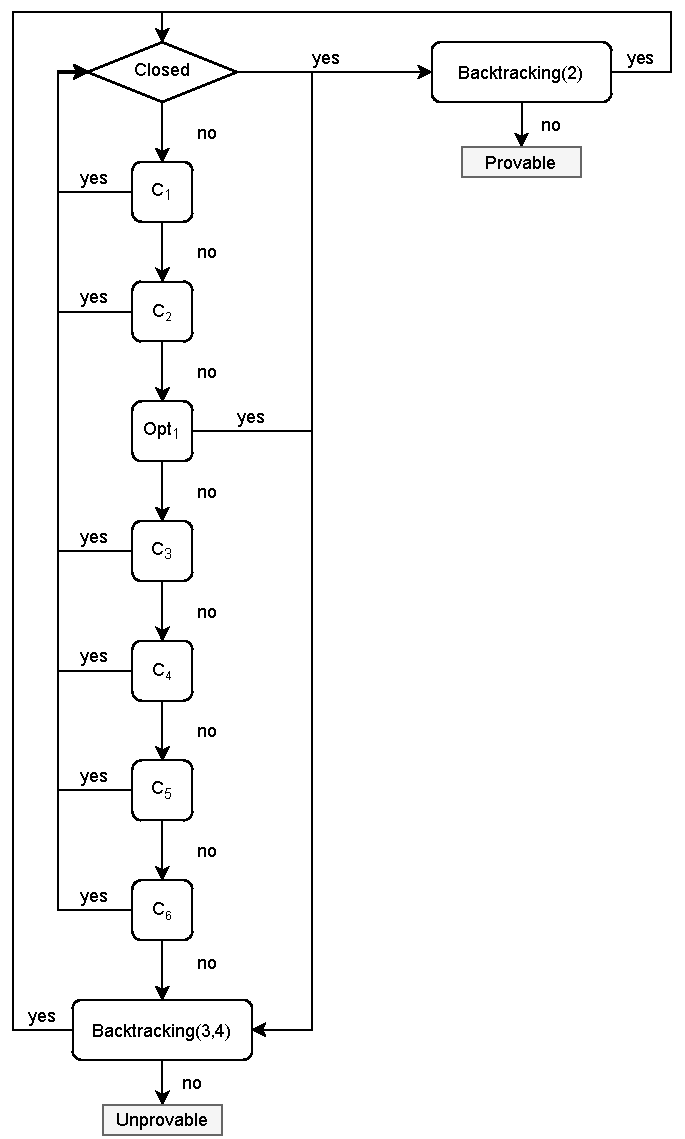
\includegraphics[scale = 1]{img/pitp.pdf}
  \caption{Flowchart di PITP. Si noti che $Opt_2$ è eseguito con $C_2$ e $Opt_3$
    con $backtracking(3,4)$, avendo la ricerca di $\tau$ tale che $H=\tau(H')$ e
    $\tau = \tau^{-1}$. Se il tableau chiude la formula è dimostrabile.}
  \label{fig:pitp}
\end{figure}
\section{Sviluppi Futuri}
Non si è mai provato a fare un'implementazione predicativa del prover,
che è quindi un campo aperto anche se con forti difficoltà all'orizzonte.
Un'altra aggiunta interessante sarebbe parallelizzare l'esecuzione e in merito
sono stati fatti alcuni tentativi anche se non ci sono stati risultati
sensazionali come attesi. Lo studio del perché non si abbiano ottimi vantaggi è
ancora in corso.
Addirittura dei campi aperti sono algoritmi quantistici ma anche di
intelligenza artificiale, anche se studi nel mondo in merito ad entrambi non
stanno portando a grandi risultati, avendo che PITP resta ancora il migliore,
nonostante sia sequenziale e con tecniche tradizionali e di backtracking. Il
problema del deep learning è che non si può dire nulla a priori su una formula
intuizionistica. 
Un'altra idea di Moscato è usare un cluster di formule decidibili e uno di
formule non decidibili.
\end{document}

% LocalWords:  clock Bayesana machine learning Bayes riscalare Prolog Morgan
% LocalWords:  condizionalmente l'algoritmicità tableaux intuizionisticamente
% LocalWords:  l'istanziazione Kripke contromodello sottoformule Kolmogorov sse
% LocalWords:  Glivenko incorporariamo sequenti implicazionale implicazionali
% LocalWords:  branch arietà un'istanziazione contromodelli definibilità Kuroda
% LocalWords:  backtracking Fitting Miglioli vedisi modalizzata Lewis jumping
% LocalWords:  modalizzare Demodalizzare modalizzate demodalizzare modalisti
% LocalWords:  necessitazione necessitazioni Mondadori benchmark Avellone
% LocalWords:  tableau
